\documentclass[12pt]{article}

% feina a fer per al curs 2010-2011
% 1) l'exercici proposat de maximitzar una funció de dues variables és difícil i cal treballar-lo. Mirar bé el mètode d'steepest descent i el de Newton Raphson (els dos proposats a l'exercici). Mirar també d'entendre correctament el mètode d'optimitzar la funció de Davidson. Mirar una bona explicació a http://linneus20.ethz.ch:8080/1_5_3.html#SECTION00253100000000000000 Fer un dibuis que mostri el concepte de "constant norm", entès com un radi determinat al voltant d'x, un radi donat per l'stepsize. És prou entendor així
\usepackage{framed}
\usepackage{url}
\usepackage{ifthen}
\usepackage{longtable}
\usepackage{fancyvrb}
\usepackage[catalan]{babel}
\usepackage{cancel}
\usepackage{enumitem}
\usepackage[thinc]{esdiff}

%\usepackage[utf8]{inputenc}
\usepackage[catalan]{babel}
\usepackage{lmodern}
\usepackage{diagbox}
\usepackage{amsmath,amsthm,amsfonts,amssymb,amscd}
%\newcommand*\diff{\mathop{}\!\mathrm{d}}
%\newcommand*\Diff[1]{\mathop{}\!\mathrm{d^#1}}
\usepackage[]{systeme}
\usepackage[arrowdel]{physics}
\usepackage{multirow,booktabs}
\usepackage[dvipsnames,table]{xcolor}
%\usepackage{fullpage}
\usepackage{lastpage}
\usepackage{graphicx}
\graphicspath{{../figures/}}

\usepackage{enumitem}
\usepackage{fancyhdr}
\setlength{\headheight}{14pt}
\usepackage{mathrsfs}
\usepackage{wrapfig}
\usepackage{setspace}
\usepackage{calc}
\usepackage{multicol}
\usepackage{textcomp}
\usepackage{gensymb}
\usepackage{listings}
\usepackage{siunitx}

\usepackage{cancel}
%\usepackage[retainorgcmds]{IEEEtrantools}
\usepackage[margin=3cm]{geometry}
\usepackage{amsmath}
\newlength{\tabcont}
\setlength{\parindent}{0.0in}
\setlength{\parskip}{0.05in}
\usepackage{empheq}
\usepackage{framed}
\usepackage{mdframed}

\usepackage[most]{tcolorbox}
% \usepackage{chemfig,chemmacros,chemnum}
% \usepackage{chemformula}

%\usepackage{unicode-math}

\usepackage{tcolorbox}
\usepackage{url}
  \let\oldurl\url
\usepackage{hyperref}
  \let\linkurl\url
  \let\url\oldurl

% \usepackage[
% backend=biber,
% citestyle=numeric-comp
% ]{biblatex}
% \addbibresource{/Users/556079/Documents/teaching.bib}


%\chemsetup[chemformula]{format=\sffamily}
%\renewcommand*\printatom[1]{\ensuremath{\mathsf{#1}}}
%\setatomsep{2em}
%\setdoublesep{.6ex}
%\setbondstyle{semithick}
%\colorlet{shadecolor}{orange!15}
% \parindent 0in
% \parskip 12pt
% \geometry{margin=1in, headsep=0.25in}
% \theoremstyle{definition}
% \newtheorem{defn}{Definition}
% \newtheorem{reg}{Rule}
% \newtheorem{exer}{Exercise}
% \newtheorem{note}{Note}
%\RequirePackage{mathrsfs}
%\RequirePackage[psamsfonts]{amsfonts} %for Y&Y BSR AMS fonts
\RequirePackage{amsmath,amsfonts,amsthm,amssymb}
\RequirePackage{setspace}
\RequirePackage{fancyhdr}
\RequirePackage{lastpage}
\RequirePackage{extramarks}
\RequirePackage{chngpage}
\RequirePackage{soul}


\usepackage{graphicx}
\usepackage{multicol}
\usepackage{hyperref}
\usepackage{makecell}
\usepackage{fancybox}

%\RequirePackage[dvipsnames]{xcolor}
%\RequirePackage{graphicx,float,wrapfig}
\RequirePackage{pgf,tikz}
\usepackage{pgfplots}
%\usetikzlibrary{arrows,automata}
%\RequirePackage{pstricks}
%\RequirePackage[text]{amsthm}
%\RequirePackage{array}
%\RequirePackage{amscd}
%\RequirePackage{array}\RequirePackage{dcolumn}
%\putfig{3.5truein}{PSfig1.3}{Peter's winnings in 40 plays of heads or tails.}{fig 1.3}

% \newcommand*{\DIRFig}{../../../../talks/figures}
% \newcommand{\barefig}[2]{\makebox{\includegraphics*[width=#2] {\DIRFig/#1}}}
% \newcommand{\putfig}[4]
% {\begin{figure}
% \centerline{\barefig{#2}{#1}}
% \caption{#3}
% \label{#4}
% \end{figure}}

\newcommand{\dif}{\, \mathop{}\!\mathrm{d}}
\newcommand{\dx}{\, dx}
\newcommand{\dy}{\, dy}
\newcommand{\dt}{\, dt}
\newcommand{\dth}{\, d\theta}
\newcommand{\dr}{\, dr}
\newcommand{\du}{\, du}
\newcommand\uvec[1]{\textbf{#1}}
\newcommand{\iu}{\hat{\uvec{i}}}
\newcommand{\ju}{\hat{\uvec{j}}}
\newcommand{\ku}{\hat{\uvec{k}}}

% \newcommand{\emx}[1]{{\em{#1}\/}}
% \newcommand{\abin}{{\it ab initio}}
% \newcommand{\bs}{\boldsymbol}
% \newcommand{\citenum}{\cite}
% \newcommand{\dGo}{\ensuremath{\Delta G_0}}
% \newcommand{\dG}[2]{\ensuremath{\Delta G_{\rm #1}^{\rm #2}}}
% \newcommand{\dX}[3]{\ensuremath{\Delta #1_{\rm #2}^{\rm #3}}}
% \newcommand{\ddgo}[1]{\ensuremath{\Delta \Delta G_{\rm solv}^{\rm #1}}}
% \newcommand{\ddgstarcat}{\ensuremath{\Delta \Delta g^{\ddagger}_{\rm cat}}}
% \newcommand{\ddgstar}{\ensuremath{\Delta \dgstar}}
% \newcommand{\ddgt}[2]{\ensuremath{\Delta \Delta G_{\rm solv}^{\rm #1, \rm #2}}}
% \newcommand{\ddsstarprime}{\ensuremath{(\Delta \dsstar)'}}
% \newcommand{\deltaepsel}{\ensuremath{\Delta \varepsilon_{\rm el}}}
% \newcommand{\deltaeps}{\ensuremath{\Delta \varepsilon}}
% \newcommand{\dgab}[2]{\ensuremath{\Delta g_{\rm #1}^{\rm #2}}}
% \newcommand{\dga}[1]{\ensuremath{\Delta g_{\rm #1}}}
% \newcommand{\dgb}[1]{\ensuremath{\Delta g^{\rm #1}}}
% \newcommand{\dgcage}{\ensuremath{\Delta g_{\rm cage}}}
% \newcommand{\dgcat}{\ensuremath{\Delta g_{\rm cat}}}
% \newcommand{\dgsoltsatsa}{\ensuremath{\dgsol (\rm TSA)_{\rm TSA}}}
% \newcommand{\dgsoltstsa}{\ensuremath{\dgsol (\rm TS)_{\rm TSA}}}
% \newcommand{\dgsoltsts}{\ensuremath{\dgsol (\rm TS)_{\rm TS}}}
% \newcommand{\dgsol}{\ensuremath{\Delta G_{\rm sol}}}
% \newcommand{\dgstarcage}{\ensuremath{\dgstar_{\rm cage}}}
% \newcommand{\dgstarcat}{\ensuremath{\dgstar_{\rm cat}}}
% \newcommand{\dgstarw}{\ensuremath{\dgstar_{\rm w}}}
% \newcommand{\dgstar}{\ensuremath{\Delta g^{\ddagger}}}
% \newcommand{\dgw}{\ensuremath{\Delta g_{\rm w}}}
% \newcommand{\dg}[2]{\ensuremath{\Delta g_{\rm #1}^{\rm #2}}}
% \newcommand{\dino}{\texttt{DINO}}
% \newcommand{\dsstarcageprime}{\ensuremath{(\dsstarcage)'}}
% \newcommand{\dsstarcage}{\ensuremath{\dsstar_{\rm cage}}}
% \newcommand{\dsstarcatprime}{\ensuremath{(\dsstarcat)'}}
% \newcommand{\dsstarcat}{\ensuremath{\dsstar_{\rm cat}}}
% \newcommand{\dsstarwprime}{\ensuremath{(\dsstarw)'}}
% \newcommand{\dsstarw}{\ensuremath{\dsstar_{\rm w}}}
% \newcommand{\dsstar}{\ensuremath{\Delta S^{\ddagger}}}
% \newcommand{\eg}{{\it e.g.}}
% \newcommand{\etal}{{\it et al.}}
% \newcommand{\gamess}{\texttt{GAMESS}}
% \newcommand{\gauss}{\texttt{GAUSSIAN} 98}
% \newcommand{\golpe}{\texttt{GOLPE}}
% \newcommand{\grid}{\texttt{GRID}}
% \newcommand{\ie}{{\it i.e.}}
% \newcommand{\ith}{{\it i}$^{\rm th}$\ }
% \newcommand{\kbt}{\ensuremath{k_{\rm B} T}}
% \newcommand{\kb}{\ensuremath{k_{\rm B}}}
% \newcommand{\kcage}{\ensuremath{k_{\rm cage}}}
% \newcommand{\kcatkm}{\ensuremath{k_{\rm cat}/K_{\rm M}}}
% \newcommand{\kcat}{\ensuremath{k_{\rm cat}}}
% \newcommand{\km}{kcal mol$^-1$}
% \newcommand{\knon}{\ensuremath{k_{\rm non}}}
% \newcommand{\kw}{\ensuremath{k_{\rm w}}}
% \newcommand{\mepsim}{\texttt{MEPSIM}}
% \newcommand{\mgp}[1]{\marginpar{\scriptsize{#1}}}
% \newcommand{\mipsim}{\texttt{MIPSIM}}
% \newcommand{\mola}{\texttt{MOLARIS}}
% \newcommand{\msms}{\texttt{MSMS}}
% \newcommand{\pdras}{p21$^{\rm ras}$}
\newcommand{\rgran}{\ensuremath{\mathbb{R}}}
\newcommand{\rx}[2]{\ensuremath{#1_{\rm #2}}}
\newcommand{\vs}{{\it vs.}}
\newcommand{\z}[1]{\ensuremath{\mathbf{#1}}}
\newcommand{\composed}[2]{#1\mathbin\circ #2}
\newcommand{\wrt}[1]{{\mbox{\scriptsize w.r.t. \( #1 \)} }}
\newcommand{\polyspace}{\mathcal{P}}
\newcommand{\matspace}{\mathcal{M}}
%\newcommand{\C}{\mathbb{C}}
\newcommand{\N}{\mathbb{N}}
\newcommand{\Q}{\mathbb{Q}}
\newcommand{\Z}{\mathbb{Z}}
\renewcommand{\Re}{\mathbb{R}}
\newcommand{\rtres}{\ensuremath{\Re^3}}
\newcommand{\union}{\cup}
\newcommand{\dotprod}{\cdot}
\newcommand*\pkg[1]{\textsf{#1}}

%\def\checkmark{\tikz\fill[scale=0.4](0,.35) -- (.25,0) -- (1,.7) -- (.25,.15) -- cycle;}


\newcommand{\trans}[1]{{#1}^{\ensuremath{\mathsf{T}}}} % transpose
\newcommand{\nbyn}[1]{\ensuremath{#1 \! \times \! #1 }}
\newcommand{\nbym}[2]{#1 \! \times \! #2 }       % Use in math mode.
\newcommand{\cat}[2]{#1\!\mathbin{\raise.6ex\hbox{\( {}^\frown \)}}\!#2}
\newcommand{\generalmatrix}[3]{ %arg1: low-case letter, arg2: rows, arg3: cols
               \left(
                  \begin{array}{cccc}
                    #1_{1,1}  &#1_{1,2}  &\ldots  &#1_{1,#2}  \\
                    #1_{2,1}  &#1_{2,2}  &\ldots  &#1_{2,#2}  \\
                              &\vdots                         \\
                    #1_{#3,1} &#1_{#3,2} &\ldots  &#1_{#3,#2}
                  \end{array}
               \right)  }
\newcommand{\colvec}[1]{\begin{pmatrix} #1 \end{pmatrix}}
\newcommand{\pr}[1]{\ensuremath{\mathrm{Pr}(#1)}}
\newcommand{\rep}[2]{ {\rm Rep}_{#2}(#1) }
\newcommand{\mapsunder}[1]{\stackrel{#1}{\longmapsto}}
\newcommand{\map}[3]{\mbox{$#1\colon #2\to #3$}}
\newcommand{\identity}{\mbox{id}}
\newcommand{\stdbasis}{{\cal E}}
\newcommand{\sequence}[1]{ \langle#1\rangle }
\newcommand{\spacer}{\rule[-3mm]{0mm}{8mm}}
\newcommand{\email}[1]{\url{#1}}
\newcommand{\zero}{\vec{0}}
\newcommand{\proj}[2]{\mbox{proj}_{#2}({#1}) }
%\AtBeginDocument{\newlength{\heightofcdot}
%\newlength{\widthofcdot}
%\settoheight{\heightofcdot}{$\cdot$}
%\settowidth{\widthofcdot}{$\cdot$}
%\newsavebox{\dotprodcircle}
%\savebox{\dotprodcircle}{\includegraphics{dotprod.1}}
%\newcommand{\dotprod}{\mathbin{\raisebox{.5\heightofcdot}{%
%          \makebox[\widthofcdot]{$\smash{\usebox{\dotprodcircle}}$}}}}}
\newcommand{\spanof}[1]{\relax [#1\relax ]} % no optional argument!
\newcommand{\set}[1]{\mbox{$\{#1\}$}} \newcommand{\suchthat}{\bigm|}
\newcommand{\deter}[1]{ \mathchoice{\left|#1\right|}{|#1|}{|#1|}{|#1|} }
\newcommand{\secuence}[1]{ \langle#1\rangle }
\newcommand{\basis}[2]{\secuence{\vec{#1}_1,\ldots,\vec{#1}_{#2}}}



%--------linsys
%  Use as \begin{linsys}{3}
%           x &+ &3y &+ &a &= &7 \\
%           x &- &3y &+ &a &= &7
%         \end{linsys}
% Remark: TeXbook pp. 167-170 says to put a medmuskip around a +; and that's
% 4/18-ths of an em.  Why does 2/18-ths of an em work?  I don't know, but
% comparing to a regular displayed equation suggests it is right.
% (darseneau says LaTeX puts in half an \arraycolsep.)
\newenvironment{linsys}[2][m]{%
\setlength{\arraycolsep}{.1111em} % p. 170 TeXbook; a medmuskip
\begin{array}[#1]{@{}*{#2}{rc}r@{}}
}{%
\end{array}}


%\newtheorem{teorema}{Teorema}
%\newtheorem{exercici}{Exercici}
%\newtheorem{definicio}{Definici\'o}
%\newtheorem{theorem}{Theorem}
\newtheorem{exercise}{Exercise}
%\newtheorem{definition}{Definition}

\newcounter{EXMP}
\newenvironment{EXMP}[1][]{\definecolor{shadecolor}{rgb}{0.6,0.6,0.6}
							\begin{shaded}\refstepcounter{EXMP}\par\medskip\noindent%
   							\textbf{EXAMPLE~\theEXMP. #1} \rmfamily}
   							{\end{shaded}\medskip}

\newcounter{BOXT}
\newenvironment{BOXT}[1][]{\definecolor{shadecolor}{rgb}{0.8,0.8,0.8}
							\begin{shaded}\refstepcounter{BOXT}\par\medskip\noindent%
   							\textbf{BOX~\theBOXT. #1} \rmfamily}
   							{\end{shaded}\medskip}

\parskip 4mm


\usepackage{makeidx}
\makeindex


% margins
\topmargin=-0.45in      %
\evensidemargin=0in     %
\oddsidemargin=0in      %
\textwidth=6in        %
\textheight=8.5in       %
\headsep=0.25in         %

% header and footer
\pagestyle{fancy}       %                %
\cfoot{
\includegraphics[width=4.8cm]{FCTE}}                %
\rfoot{\thepage}        %
\renewcommand\headrulewidth{0.4pt}   %
\renewcommand\footrulewidth{0.4pt}   %

%\setcounter{section}{-1}

\theoremstyle{definition}
\newtheorem{thm}{Theorem}
\newtheorem{dfn}{Definition}
\newtheorem{lem}{Lemma}
\newtheorem{prp}{Proposition}



%%%%%%%%%%%%%%%%%%%%%%%%%%%%%%%%%%%%%%%%%
%%%%%%%%%%%%%%%%%%%%%%%%%%%%%%%%%%%%%%%%%
% lecturer or student text
% in principle the lecturer text includes some examples to be done in the c lass
\newboolean{LECT}
\setboolean{LECT}{false}
\setboolean{LECT}{true}
%%%%%%%%%%%%%%%%%%%%%%%%%%%%%%%%%%%%%%%%%
%%%%%%%%%%%%%%%%%%%%%%%%%%%%%%%%%%%%%%%%%

\newenvironment{lect}{ %
	\definecolor{shadecolor}{rgb}{1.0,0.8,0.8} %
	\begin{shaded} %
	\textcolor{BrickRed}{\bf Resultat\\}%

} %
{ %
	\end{shaded}
} %

\newcommand{\lct}[1]{\ifthenelse{\boolean{LECT}}{\begin{lect} #1 \end{lect}}{}}



%%%%%%%%%%%%%%%%%%%
% ANGLÈS
%%%%%%%%%%%%%%%%%%%

%\newcommand{\problemName}{}%
%\newcounter{problemCounter}%
%\newenvironment{problem}[1][Problem \arabic{problemCounter}]%
%	{\stepcounter{problemCounter}%
%		\renewcommand{\problemName}{#1}%
%		\section*{\problemName}%
%		\nobreak\extramarks{\problemName}{\problemName continued on next page\ldots}\nobreak%
%		\nobreak\extramarks{\problemName (continued)}{\problemName continued on next page\ldots}\nobreak}%
%	{\nobreak\extramarks{\problemName (continued)}{\problemName continued on next page\ldots}\nobreak%
%		\nobreak\extramarks{\problemName}{}\nobreak}%

\newenvironment{example}{ %merges with the question content
} %


\newenvironment{introduction}{ %
	\definecolor{shadecolor}{rgb}{1.0,1.0,0.8} %
	\begin{shaded} %
	% \textcolor{BrickRed}{\bf Introduction\\}%
} %
{ %
	\end{shaded}
} %


%%%%%%%%%%%%%%%%%%%
% CATALÀ
%%%%%%%%%%%%%%%%%%%
\newtheorem{teorema}{theorem}
\newenvironment{definicio}{ %
	\definecolor{shadecolor}{rgb}{0.9,1.0,0.8} %
	\begin{shaded} %
	\textcolor{OliveGreen}{\bf Definicio\\}%
} %
{ %
	\end{shaded}
} %

%veure http://en.wikibooks.org/wiki/LaTeX/Advanced_Topics
\newcounter{myc}
%environment for exercises in the class notes
\newenvironment{exr}{ %
    \addtocounter{myc}{1}
	\definecolor{shadecolor}{rgb}{0.9,1.0,0.8} %
	\begin{shaded} %
	\textcolor{OliveGreen}{\bf Exercici \arabic{myc}\\}%
} %
{ %
	\end{shaded}
} %
%environment for questions in exams
\newenvironment{qst}{ %
    \addtocounter{myc}{1}
	\definecolor{shadecolor}{rgb}{0.9,1.0,0.8} %
	\begin{shaded} %
	\textcolor{OliveGreen}{\bf Qüestió \arabic{myc}\\}%
} %
{ %
	\end{shaded}
} %


\usepackage[lastexercise]{exercise}
% \renewcommand{\listexercisename}{\'{I}ndex d'exercicis}
% \renewcommand{\ExerciseListName}{Ex.}  % titol a cada exercici
% \renewcommand{\AnswerListName}{Soluci\'{o}}
% \renewcommand{\AnswerName}{Soluci\'{o} de l'exercici}
% \renewcommand{\ExerciseName}{Exercici}  % títol que apareix al llistat d'exercicis
% \renewcommand{\ExerciseHeaderTitle}{\ExerciseTitle \quad---\quad \medskip}
% \renewcommand{\ExerciseListHeader}{
%         \shadowbox*{
%                 \ExerciseHeaderDifficulty%
%                 \textbf{\ExerciseListName\ \ExerciseHeaderNB%
%                 \ --- \ \ExerciseHeaderTitle}%
%                 \medskip\ExerciseHeaderOrigin%
%                 \ignorespaces
%         }
% }

\makeatletter
% remove the faulty \expandafter
\patchcmd{\@@@ExeEnv}
  {\theExercise\ \expandafter}
  {\theExercise\ }
  {}{}
\patchcmd{\@@@ExeCmd}
  {\theExercise\ \expandafter}
  {\theExercise\ }
  {}{}
% remove \itshape
\patchcmd{\@@@ExeEnv}
  {\itshape}
  {}
  {}{}
\patchcmd{\@@@ExeCmd}
  {\itshape}
  {}
  {}{}
\makeatother
\usepackage{amsmath, amssymb, amsthm}

\usepackage[catalan]{babel}
\usepackage{graphicx}
\graphicspath{{../figures/}}

\begin{document}

\lstset{language=Matlab,%
    basicstyle=\color{red},
    breaklines=true,%
    morekeywords={matlab2tikz},
    keywordstyle=\color{blue},%
    morekeywords=[2]{1}, keywordstyle=[2]{\color{black}},
    identifierstyle=\color{black},%
    stringstyle=\color{purple},
    commentstyle=\color{green},%
    showstringspaces=false,%without this there will be a symbol in the places where there is a space
    numbers=left,%
    numberstyle={\tiny \color{black}},% size of the numbers
    numbersep=9pt, % this defines how far the numbers are from the text
    emph=[1]{for,end,break},emphstyle=[1]\color{red}, %some words to emphasise
    emph=[2]{word1,word2}, emphstyle=[2]{style},
}


\title{Exercicis Resolts \\ \large MATEMÀTIQUES I \\ Grau en Enginyeria Mecatrònica 
\author{Jordi Villà i Freixa}\thanks{Adreça electrònica: \texttt{jordi.villa@uvic.cat}}
\begin{center}
\includegraphics[width = 60mm]{FCTE}\end{center}}
\date{Darrera modificació: \today}
\maketitle

\tableofcontents
\newpage

Aquest és un llistat d'exercicis recollits de diverses fonts. Si hi detecteu algun error feu-me'l arribar i corregiré el document.
%
\begin{ExerciseList}

\section{Àlgebra lineal}


\Exercise Quins dels següents conjunts de vectors formen una base de $\mathbb{R}^3$?
  \begin{enumerate}[label=(\alph*)]
    \item $\{(1,-2,3),(0,1,1),(-1,1,2)\}$
    \item $\{(1,-2,3),(0,1,1),(1,-3,2)\}$
    \item $\{(1,-2,3),(0,1,1),(0,0,1)\}$
  \end{enumerate}

\Answer L'espai vectorial $E={x\in \mathbb{R}^3}$ té dimensió 3. Això vol dir que si trobem un conjunt de tres vectors linealment independents en formaran una base:
\begin{enumerate}[label=(\alph*)]
  \item $\{(1,-2,3),(0,1,1),(-1,1,2)\}$
  Fem el determinant de la matriu formada pels tres vectors:
  \begin{eqnarray*}
    det \begin{pmatrix}1&0&-1\\-2&1&1\\3&1&2\end{pmatrix}&=&
    +[1\cdot1\cdot2+0\cdot1\cdot3+(-2)\cdot1\cdot(-1)]-\\
    &&-[(-1)\cdot1\cdot3+0\cdot(-2)\cdot2+1\cdot1\cdot1]\\
    &=&4-(-2)=6 \neq 0
  \end{eqnarray*}
  Per tant, són linealment independents i formen una base d'$\mathbb{R}^3$.
  \blacksquare

  \item $\{(1,-2,3),(0,1,1),(1,-3,2)\}$
  \begin{eqnarray*}
    det \begin{pmatrix}1&0&1\\-2&1&-3\\3&1&2\end{pmatrix}&=&
    +[1\cdot1\cdot2+0\cdot(-3)\cdot3+(-2)\cdot1\cdot(1)]-\\
    &&-[1\cdot1\cdot3+0\cdot(-2)\cdot2+(-3)\cdot1\cdot1]\\
    &=&0
  \end{eqnarray*}
  Per tant, són linealment dependents i no formen una base d'$\mathbb{R}^3$.
  \blacksquare

  \item $\{(1,-2,3),(0,1,1),(0,0,1)\}$
  \begin{eqnarray*}
    det \begin{pmatrix}1&0&0\\-2&1&0\\3&1&1\end{pmatrix}&=&
    1
  \end{eqnarray*}
  Per tant, són linealment independents i formen una base d'$\mathbb{R}^3$.
  \blacksquare

\end{enumerate}

\Exercise Si $\{\overrightarrow{v_1},\overrightarrow{v_2}\} = \{ (2,1),(-2,1) \}$ i $\{\overrightarrow{e_1},\overrightarrow{e_2}\} = \{ (1,0),(0,1) \}$
\begin{enumerate}
  \item Comprova que $\overrightarrow{e_1}$ i $\overrightarrow{e_2}$ és una base de $\mathbb{R}^2$.
  \item Perquè $\overrightarrow{e_1}$, $\overrightarrow{v_1}$ i $\overrightarrow{v_2}$ no són una base de $\mathbb{R}^2$?
  \item Formen una base de $\mathbb{R}^2$ els vectors $\overrightarrow{v_1}$ i $\overrightarrow{v_2}$?
  \item Quants vectors com a molt formen una base de $\mathbb{R}^2$?
  \item I d'$\mathbb{R}^3$?
\end{enumerate}

\Answer  Recordem que els vectors $\overrightarrow{v_1},\overrightarrow{v_2}, \ldots, \overrightarrow{v_n}$ són una base de l'espai vectorial al qual pertanyen quan (1) són generados de l'espai, i (2) són linealment independents.
\begin{enumerate}
\item Comprova que $\overrightarrow{e_1}$ i $\overrightarrow{e_2}$ és una base de $\mathbb{R}^2$. Ens preguntem promer si podem posar tots els vectors d'$\mathbf{R}^2$ en funció dels vectors $\overrightarrow{e_1}$ i $\overrightarrow{e_2}$:
\[(x,y) = \alpha (1,0) + \beta (0,1) \]
Es pot veure que si $x=\alpha$ i $y=\beta$ es satisfà l'equació.\\
Mirem ara si són linealment independents. Els vectors $\overrightarrow{v_1},\overrightarrow{v_2}, \ldots, \overrightarrow{v_n}$ són {\bf linealment dependents} si qualsevol d'ells es pot escriure com a combinació lineal de la resta. En cas contrari els anomenem {\bf linealment independents}. La definició equival a veure si en l'expressió
\[(0,0) = \alpha (1,0) + \beta (0,1) \]
hi ha alguna solució per a $\alpha$ i $\beta$ diferent de la trivial $\alpha=0$ i $\beta=0$.
Plantejant el sistema d'equacions:
\[
  \systeme*{0=\alpha\cdot 1 + \beta\cdot 0, 0=\alpha\cdot 0 + \beta\cdot 1}
\]
veiem que l'única solució possible és que, justament, $\alpha=0$ i $\beta=0$. Per tant, són {\bf linealment independents}.\\
Per tant, $\left\{\overrightarrow{e_1},\overrightarrow{e_2}\right\}$ forma una base d'$\mathbf{R}^2$.


\item Perquè $\overrightarrow{e_1}$, $\overrightarrow{v_1}$ i $\overrightarrow{v_2}$ no són una base de $\mathbb{R}^2$?
Són, de fet, un conjunt generador de $\mathbb{R}^2$, però no en formen base perquè no són linealment independents. Plantegem l'equació
\[(0,0) = \alpha (1,0) + \beta (0,1) +\gamma (-2,1)\]
que duu al sistema d'equacions:
\[
  \systeme*{0=\alpha\cdot 1 + \beta\cdot 0 - \gamma\cdot 2, 0=\alpha\cdot 0 + \beta\cdot 1 + \gamma \cdot 1}
\]
que podem reduir a 
\[
  \systeme*{0=\alpha - 2\gamma, 0=\beta + \gamma}
\]
Es tracta d'un sistema de dues equacions amb tres incògnites. El sistema és compatible (té solució) perquè sempre podem dir que $\alpha=\beta=\gamma=0$ (que anomenem solució trivial), però també podem veure que si donem un valor arbitrari a, per exemple, $\gamma$, obtenim $\alpha=2\gamma$ i $\beta=-\gamma$. Per tant, la solució trivial no és l'única possible i, per tant, són linealment dependents. Dit d'una altra manera, a $\mathbf{R}^2$ només hi "cap" una base de dos vectors, no tres.
\item Formen una base de $\mathbb{R}^2$ els vectors $\overrightarrow{v_1}$ i $\overrightarrow{v_2}$?
En ser dos només ens cal veure si són linealment independents. Plantegem
\[(0,0) = \alpha (2,1) + \beta (-2,1) \]
i obtenim
\[
  \systeme*{0=2\alpha- 2 \beta, 0=\alpha + \beta}
\]
Sumant la segona equació dos cops a la primera obtenim
\[
  \systeme*{0=4\alpha }
\]
Per tant, la solució $\alpha=\beta=0$ ens fa concloure que sñón linealment independents i, per tant, formen base de $\mathbb{R}^2$
\item Quants vectors com a molt formen una base de $\mathbb{R}^2$?
Un màxiom de dos poden ser L.I. i seguir generant tot l'espai.
\item I d'$\mathbb{R}^3$?
Pel mateix raonament, 3 vectors.
\end{enumerate}
\blacksquare


\Exercise Trobeu les equacions cartesianes dels plans següents:
\begin{enumerate}
  \item El pla que passa pels punts $(0,0,0)$, $(1,2,3)$ i $(-2,3,3)$.
  \item El pla que passa pel punt $(2,1,2)$ i té per vector normal $\uvec{n}=2\uvec{i}+3\uvec{j}-\uvec{k}$.
  \item El pla que passa pel punt $(3,2,2)$ i és perpendicular a la recta $\frac{x-1}{4}=y+2=\frac{z+3}{-3}$
  \item El pla que conté les rectes $\frac{x-1}{2}=y-4=z$ i $\frac{x-2}{-3}=\frac{y-1}{4}=\frac{z-2}{-1}$
  \item El pla que passa pels punts $(2,2,1)$ i $(-1,1,-1)$ i és perpendicular al pla $2x-3y-z=3$
\end{enumerate}
 
\Answer Usarem que els coeficients de l'equació cartesiana del pla $Ax+By+Cz=D$ corresponen amb les coordenades del seu vector normal $\uvec{n}=A\uvec{i}+B\uvec{j}+C\uvec{k}$

\begin{enumerate}
  \item El pla que passa pels punts $(0,0,0)$, $(1,2,3)$ i $(-2,3,3)$.

El vector perpendicular al pla es por calcular amb el producte vectorial de dos vectors del pla com, per exemple: $\uvec{u}=(1,2,3)-(0,0,0)$ i $\uvec{v}=(-2,3,3)-(0,0,0)$. Així,

\[
\uvec{u} \times \uvec{v}=
\begin{vmatrix}
\uvec{i} & \uvec{j} & \uvec{k} \\
1 & 2 & 3\\
-2 & 3 & 3
\end{vmatrix}=
(6\uvec{i}-6\uvec{j}+3\uvec{k})-(9\uvec{i}+3\uvec{j}-4\uvec{k})=-3\uvec{i}-9\uvec{j}+7\uvec{k}
\]

Per tant, l'equació serà de la forma: $-3x-9y+7z=D$. Com que el pla passa pel punt $(0,0,0)$, l'equació buscada és:
\[
-3x-9y+7z=0
\]

  \item El pla que passa pel punt $(2,1,2)$ i té per vector normal $\uvec{n}=2\uvec{i}+3\uvec{j}-\uvec{k}$.

El pla tindrà la forma $2x+3y-z=D$. Substituint el punt donat obtenim el valor de $D$:
\[
2\cdot2+3\cdot1-2=D=5
\]
Per tant, el pla buscat és:
\[
2x+3y-z=5
\]

  \item El pla que passa pel punt $(3,2,2)$ i és perpendicular a la recta $\frac{x-1}{4}=y+2=\frac{z+3}{-3}$

El vector normal al pla és el director de la recta i, per tant: $4x+y-3z=D$. Substituint el punt donat obtenim el valor de $D$:
\[
4\cdot3+2-3\cdot2=D=8
\]
Per tant, el pla buscat és:
\[
4x+y-3z=8
\]

  \item El pla que conté les rectes $\frac{x-1}{2}=y-4=z$ i $\frac{x-2}{-3}=\frac{y-1}{4}=\frac{z-2}{-1}$

Usarem els  vectors directors de les dues rectes per trobar el vector normal al pla.

\[
\uvec{u} \times \uvec{v}=
\begin{vmatrix}
\uvec{i} & \uvec{j} & \uvec{k} \\
2 & 1 & 1\\
-3 & 4 & -1
\end{vmatrix}=
(-1\uvec{i}-3\uvec{j}+8\uvec{k})-(4\uvec{i}-2\uvec{j}-3\uvec{k})=-5\uvec{i}-\uvec{j}+11\uvec{k}
\]

El pla tindrà la forma $-5x-y+11z=D$. Podem ara agafar qualsevol punt dels que estan continguts a les dues rectes. Per exemple, agafant-lo de l'equació contínua de la primera:
\[
-5\cdot1-4+11\cdot0=D=-9
\]
Per tant, el pla buscat és:
\[
-5x-y+11z=-9
\]



  \item El pla que passa pels punts $(2,2,1)$ i $(-1,1,-1)$ i és perpendicular al pla $2x-3y-z=3$

Un dels vecotrs directors del pla buscat serà el normal del pla perpendicular: $\uvec{u}=(2,-3.-1)$. L'altre, elpodem obtenir a partir dels dos punts donats: $\uvec{v}=(-1,1,-1)-(2,2,1)=(-3,-1,-2)$. Ara podem calcular el vector normal al pla demanat:

\[
\uvec{u} \times \uvec{v}=
\begin{vmatrix}
\uvec{i} & \uvec{j} & \uvec{k} \\
2 & -3 & -1\\
-3 & -1 & -2
\end{vmatrix}=
(6\uvec{i}+3\uvec{j}-2\uvec{k})-(\uvec{i}-4\uvec{j}+9\uvec{k})=5\uvec{i}+7\uvec{j}-11\uvec{k}
\]

El pla tindrà la forma $5x+7y-11z=D$. Podem ara agafar qualsevol punt dels que estan continguts a les dues rectes.
\[
5\cdot(-1)+7\cdot1-11\cdot(-1)=D=13
\]
Per tant, el pla buscat és:
\[
5x+7y-11z=13
\]


\end{enumerate}

\Exercise Troba la combinació lineal que genera $\vec{u}=(2,1)$ a partir de
\begin{enumerate}
  \item  $\{\overrightarrow{v_1},\overrightarrow{v_2}\} = \{\overrightarrow{e_1},\overrightarrow{e_2}\} = \{ (1,0),(0,1) \}$; 
  \item i si $\{\overrightarrow{v_1},\overrightarrow{v_2}\} = \{ (2,1),(-2,1) \}$?
\end{enumerate}

\Answer Recordem que un vector $\vec{u}$ és una {\bf combinació lineal} dels vectors $\overrightarrow{v_1},\overrightarrow{v_2}, \ldots , \overrightarrow{v_n}$ si existeixen nombres reals $\lambda_1, \lambda_2, \ldots, \lambda_n$ que satisfan:
\[\vec{u} = \lambda_1 \overrightarrow{v_1} + \lambda_2 \overrightarrow{v_2} + \cdots \lambda_n \overrightarrow{v_n}\]

\begin{enumerate}
  \item Hem de trobar els coeficients que satisfan 
  \[\vec{u} = \lambda_1 \overrightarrow{v_1} + \lambda_2 \overrightarrow{v_2} \]
  Substituint:
  \[(2,1)=\lambda_1 (1,0) + \lambda_2 (0,1)\]
  d'on, clarament, $\lambda_1=2$ i $\lambda_2=1$.
  \item En aquest cas:
  \[\vec{u} = \lambda_1 \overrightarrow{v_1} + \lambda_2 \overrightarrow{v_2} \]
  Substituint:
  \[(2,1)=\lambda_1 (2,1) + \lambda_2 (2,-1)\]
  d'on obtenim $\lambda_1=1$ i $\lambda_2=0$.
\end{enumerate}
\blacksquare


\Exercise Si $\{\overrightarrow{v_1},\overrightarrow{v_2}\} = \{ (2,1),(-2,1) \}$ i $\{\overrightarrow{e_1},\overrightarrow{e_2}\} = \{ (1,0),(0,1) \}$
\begin{enumerate}
  \item Pots escriure $\overrightarrow{e_2}$ en funció de $\{\overrightarrow{v_1},\overrightarrow{v_2}\}$?
  \item Pots escriure $\overrightarrow{e_1}$ en funció de $\{\overrightarrow{v_1},\overrightarrow{v_2}\}$?
  \item Pots escriure $\overrightarrow{v_2}$ en funció de $\{\overrightarrow{e_1}\}$?
  \item Com són els vectors que es poden escriure com a combinació lineal de $\overrightarrow{e_1}$?
\end{enumerate}

\Answer Recordem que un vector $\vec{u}$ és una {\bf combinació lineal} dels vectors $\overrightarrow{v_1},\overrightarrow{v_2}, \ldots , \overrightarrow{v_n}$ si existeixen nombres reals $\lambda_1, \lambda_2, \ldots, \lambda_n$ que satisfan:
\[\vec{u} = \lambda_1 \overrightarrow{v_1} + \lambda_2 \overrightarrow{v_2} + \cdots \lambda_n \overrightarrow{v_n}\]

\begin{enumerate}
  \item Hem de trobar els coeficients que satisfan 
  \[\vec{e_2} = \alpha \overrightarrow{v_1} + \beta \overrightarrow{v_2} \]
  Substituint:
  \[(0,1)=\alpha (2,1) + \beta (-2,1)\]
  d'on obtenim 
  \[
    \systeme*{0=2\alpha-2\beta, 1=\alpha+\beta}
  \]
  multiplicant la segona equació per 2 i sumant-la a la primera obtenim que $2=4\alpha$, d'on $\alpha=\beta=1/2$. Per tant:
  \[\vec{e_2} = \frac{1}{2} \overrightarrow{v_1} +\frac{1}{2} \overrightarrow{v_2} \]
  \item Hem de trobar els coeficients que satisfan 
  \[\vec{e_1} = \alpha \overrightarrow{v_1} + \beta \overrightarrow{v_2} \]
  Anàlogament al que hem fet abans:
  \[(1,0)=\alpha (2,1) + \beta (-2,1)\]
  d'on obtenim 
  \[
    \systeme*{1=2\alpha-2\beta, 0=\alpha+\beta}
  \]
  multiplicant la segona equació per 2 i sumant-la a la primera obtenim que $1=4\alpha$, d'on $\alpha=1/4$ i $\beta=-1/4$. Per tant:
  \[\vec{e_2} = \frac{1}{4} \overrightarrow{v_1} -\frac{1}{4} \overrightarrow{v_2} \]
  \item Si intentem fer $\overrightarrow{v_2} = \alpha \vec{e_1}$ obtenim:
  \[
    \systeme*{-2=\alpha\cdot 1, 1=\alpha\cdot 0}
  \]
  que no té solució. 
  \item Els vectors que es poden posar com a combinació lineal de $\vec{e_1}$ són de la forma $(\alpha,0)$. És per això que en l'apartat anterior veiem que no podem posar $\overrightarrow{v_2}$ com a combinació lineal de $\vec{e_1}$.
\end{enumerate}
\blacksquare


\Exercise Si $\{\overrightarrow{v_1},\overrightarrow{v_2}\} = \{ (2,1),(-2,1) \}$ i $\{\overrightarrow{e_1},\overrightarrow{e_2}\} = \{ (1,0),(0,1) \}$
\begin{enumerate}
  \item Comprova que $\overrightarrow{e_1}$ i $\overrightarrow{e_2}$ són generadors de $\mathbb{R}^2$.
  \item Comprova que $\overrightarrow{e_1}$, $\overrightarrow{v_1}$ i $\overrightarrow{v_2}$ són generadors de $\mathbb{R}^2$.
  \item Ho són $\overrightarrow{v_1}$ i $\overrightarrow{v_2}$?
  \item Dóna exemples de conjunts de vectors d'$\mathbb{R}^2$ que generin altres vectors del mateix espai vectorial amb la forma $\{(\alpha,0):\alpha \in  \mathbb{R} \}$.
  \item Comprova que el conjunt de vectors $\{(1,0,0),(0,1,0),(0,0,1)\}$ genera $\mathbb{R}^3$.
\end{enumerate}

\Answer Els vectors $\overrightarrow{v_1},\overrightarrow{v_2}, \ldots, \overrightarrow{v_n}$ són generadors de l'espai vectorial $E$ al qual pertanyen, i diem $E=\left<\overrightarrow{v_1},\overrightarrow{v_2}, \ldots, \overrightarrow{v_n}\right>$, quan qualsevol $\vec{u}\in E$ es pot posar com a combinació lineal de $\overrightarrow{v_1},\overrightarrow{v_2}, \ldots, \overrightarrow{v_n}$:
\[\vec{u} = \lambda_1 \overrightarrow{v_1} + \lambda_2 \overrightarrow{v_2} + \cdots + \lambda_n \overrightarrow{v_n}\]


\begin{enumerate}
  \item Comprova que $\overrightarrow{e_1}$ i $\overrightarrow{e_2}$ són generadors de $\mathbb{R}^2$.
  \[\vec{u} = \alpha \overrightarrow{e_1} + \beta \overrightarrow{e_2}\]
  o, anàlogament:
  \[
    \systeme*{x=\alpha,y=\beta}
  \]
  Per tant, és obvi que podem trobar valors de $\alpha$ i $\beta$ que satisfacin aquesta expressió per a qualsevol vector $(x,y)\in \mathbb{R}^2$. 
  \item Comprova que $\overrightarrow{e_1}$, $\overrightarrow{v_1}$ i $\overrightarrow{v_2}$ són generadors de $\mathbb{R}^2$.
  \[\vec{u} = \alpha \overrightarrow{e_1} + \beta \overrightarrow{v_1} + \gamma \overrightarrow{v_2}\]
  quedant:
  \[
    \systeme*{x=\alpha+2\beta-2\gamma,y=\beta+\gamma}
  \]
  Donats  valors a $\alpha$, $\beta$ i $\gamma$ podem trobar tots els valors possibles de les components dels vectors $(x,y)$.
  \item Ho són $\overrightarrow{v_1}$ i $\overrightarrow{v_2}$?
  El mateix cas que l'apartat (1).
  \item Dóna exemples de conjunts de vectors d'$\mathbb{R}^2$ que generin altres vectors del mateix espai vectorial amb la forma $\{(\alpha,0):\alpha \in  \mathbb{R} \}$.
  $(1,0)$ o $(-3/2,0)$ serien exemples d'aquests vectors. Cal notar que no generarien tot l'espai $\mathbb{R}^2$, sinó un subespai de dimensió 1 (una recta al pla $\mathbb{R}^2$).
  \item Comprova que el conjunt de vectors $\{(1,0,0),(0,1,0),(0,0,1)\}$ genera $\mathbb{R}^3$.
  Cas anàleg a l'apartat (1).
\end{enumerate}
\blacksquare


\Exercise Si $\{\overrightarrow{v_1},\overrightarrow{v_2}\} = \{ (2,1),(-2,1) \}$ i $\{\overrightarrow{e_1},\overrightarrow{e_2}\} = \{ (1,0),(0,1) \}$
\begin{enumerate}
  \item Són $\overrightarrow{e_2}$, $\overrightarrow{v_1}$ i $\overrightarrow{v_2}$ linealment independents?
  \item Són $\overrightarrow{e_1}$, $\overrightarrow{v_1}$ i $\overrightarrow{v_2}$ linealment independents?
  \item Com són els vectors linealment dependents amb $\overrightarrow{e_1}$?
  \item Són $\overrightarrow{e_1}$ i $\overrightarrow{v_2}$ linealment independents?
  \item Són $\overrightarrow{e_1}$ i $\overrightarrow{e_2}$ linealment independents?
  \item Són $\overrightarrow{v_1}$ i $\overrightarrow{v_2}$ linealment independents?
\end{enumerate}

\Answer Els vectors $\overrightarrow{v_1},\overrightarrow{v_2}, \ldots, \overrightarrow{v_n}$ són {\bf linealment dependents} si qualsevol d'ells es pot escriure com a  combinació lineal de la resta.    
\[\vec{v_1} = \alpha \overrightarrow{v_2} + \beta \overrightarrow{v_3} + \cdots + \omega \overrightarrow{v_n}\]
En cas contrari els anomenem {\bf linealment independents}. La definició equival a veure si en l'expressió
\[\vec{0} = \lambda_1 \overrightarrow{v_1} + \lambda_2 \overrightarrow{v_2} + \cdots + \lambda_n \overrightarrow{v_n}\]
hi ha alguna solució per a $\alpha$ i $\beta$ diferent de la trivial $\lambda_1,\ldots,\lambda_n=0$.


\begin{enumerate}
  \item Són $\overrightarrow{e_2}$, $\overrightarrow{v_1}$ i $\overrightarrow{v_2}$ linealment independents?
  \[\vec{0} = \alpha \overrightarrow{v_1} + \beta \overrightarrow{v_2} + \gamma \overrightarrow{e_2}\]
  Reescrivint el sistema:
  \[
    \systeme*{0=2\alpha-2\beta, 0=\alpha+\beta+\gamma}
  \]
  Es tracta d'un sistema de dues equacions i tres incògnites, compatible perque segur que té la solució trivial ($\alpha=\beta=\gamma=0$ ) però també la solució
  \[
    \systeme*{\alpha=\delta,\beta=\delta,\gamma=0}
  \]
  Per tant, són L.D. Sempre passarà el mateix quan intentem esbrinar la dependència lineal de tres vectors qualsevols al conjunt $\mathbf{R}^2$ o de 4 vectors qualsevols al conjunt $\mathbf{R}^3$, per exemple.
  \item Són $\overrightarrow{e_1}$, $\overrightarrow{v_1}$ i $\overrightarrow{v_2}$ linealment independents?
  Veure resposta a l'apartat anterior.
  \item Com són els vectors linealment dependents amb $\overrightarrow{e_1}$?
  Qualsevol vector que en la segona component tingui qualsevol valor diferent de $0$.
  \item Són $\overrightarrow{e_1}$ i $\overrightarrow{v_2}$ linealment independents?\\
  Plantegem
  \[\vec{0} = \alpha \overrightarrow{e_1} + \beta \overrightarrow{v_2} \]
  o, el que és el mateix:
  \[
    \systeme*{0=\alpha-2\beta,0=\beta}
  \]
  El resultat del sistema és $\alpha=\beta=0$ i, per tant, són L.I..
  \item Són $\overrightarrow{e_1}$ i $\overrightarrow{e_2}$ linealment independents?
  Veure l'apartat anterior.
  \item Són $\overrightarrow{v_1}$ i $\overrightarrow{v_2}$ linealment independents?
  Veure l'apartat anterior.
\end{enumerate}
\blacksquare


\Exercise Escriu una equació de cada cas:
\begin{enumerate}
    \item Escriu equacions polinòmiques amb coeficients enters que tinguin com a solucions nombres naturals, enters, racionals, irracionals (\textit{algebraics})
    \item Escriu una equació polinòmica amb coeficients enters que tingui com a solució el número $\pi$ (\textit{transcendent})
    \item Troba una equació polinòmica amb coeficients constants sense cap nombre real com a  solució
\end{enumerate}

\Answer 
\begin{enumerate}
  \item Intuitivament, una equació algebraica és aquella en la que es pot trobar la resposta usant operacions algebraiques: addició, multipliació i extracció d'arrel.
  \[2x-1=0, \; x=\frac{1}{2}\]
  o bé
  \[x^2-2=0, \; x=\pm\sqrt{2}\]
  \item Una equació transcendent, ''transcedeix'' l'àlgebra i s'han d'usar altres operacions. Per exemple, les funcions exponencials, algorítmiques o trigonomètriques. Per definició, un número real $\alpha$ és transcendent si no és algebraic. És a dir, si no existeix cap polinomi amb coeficients enters de manera que $\alpha$ en sigui una arrel. Per tant, la pregunta no té resposta, ja que no podem construir un polinomi amb solució $\pi$. La demostració \href{https://www.gaussianos.com/como-demostrar-que-%CF%80-pi-es-trascendente/}{és complicada} i la deixo com a lectura avançada.
  \item Ens passarà sempre que la solució impliqui haver de trobar l'arrel parella d'un número negatiu:
  \[x^2+1=0, \; x=\pm\sqrt{-1}\]
  que en el conjunt dels reals no té solució. Caldria resoldre-la en el conjunt dels números complexos:
  \[x^2+1=0, \; x=\pm i\]
\end{enumerate}
\blacksquare

\Exercise Trobeu l'equació general de les rectes següents:
\begin{enumerate}
  \item La recta que passa pel punt $(1,2)$ i té per vector director el vector $\uvec{v}=(3,-1)$.
  \item La recta que passa pel punt $(0,0)$ i és paral·lela a la recta $x-y=4$.
  \item La recta que passa pel punt $(1,-2)$ i és perpendicular a la recta $x+2y+5=0$
\end{enumerate}

\Answer Cada cas el podem ractar lleugerament diferent, però totes les opcions són equivalents i bescanviables en la pràctica:
\begin{enumerate}
  \item La recta que passa pel punt $(1,2)$ i té per vector director el vector $\uvec{v}=(3,-1)$.
 
  Comencem amb l'equació contínua de la recta escrivint:
  \[
  \frac{x-1}{3}=\frac{y-2}{-1}
  \]
  D'aquí:
  \begin{eqnarray*}
    -(x-1)&=&3(y-2)\\
    3y+x-7=0
  \end{eqnarray*}

  \item La recta que passa pel punt $(0,0)$ i és paral·lela a la recta $x-y=4$.

  Si les dues rectes són paral·leles, els coeficients de la $x$ i la $y$ en l'equació general seran els mateixos i, per tant, busquem el coeficient independent a l'equació $x-y=C$. Com que la recta passa pel punt $(0,0)$, $C=0$ i la recta demanada és $x-y=0$.

  \item La recta que passa pel punt $(1,-2)$ i és perpendicular a la recta $x+2y+5=0$

  Si la recta problema és ortogonal a $x+2y+5=0$ vol dir que el producte escalar dels seus vectors directors és $0$. El vector director de la recta donada és $(2,1)$ (mira l'equació contínua del primer d'aquests tres apartats) i, per tant, un possible vector ortogonal a aquest seria $(-1,2)$.\footnote{Efectivament, $(2,1)\cdot(-1,2)=0$}. Així, novament com en l'apartat anterior, busquem el coeficient independent a l'equació $2x-2y=C$. Com que la recta problema passa pel punt $(1,-2)$, tenim que $2\cdot1-2\cdot(-2)=6=C$. Per tant, la recta buscada és $2x-2y-6=0$

\end{enumerate}
\blacksquare

\Exercise
  Aïlleu $X$, si és possible, en les equancions següents, suposant que totes les matrius són quadrades del mateix ordre i invertibles:
  \begin{enumerate}[label=(\alph*) ]
    \item $3 X^t+ (XA)^t + I = B$
    \item $(XA)^{-1}=2I+B$
    \item $AX+C=BX$
  \end{enumerate}

\Answer Usant les propietats de les operacions amb matrius:

  \begin{enumerate}[label=(\alph*) ]
    \item $3 X^t+ (XA)^t + I = B$
    \begin{eqnarray*}
      3 X^t+ (XA)^t + I &=&B\\
      (3X)^t + (XA)^t &=& B-I\\
      (3X+XA)^t &=& B-I\\
      3X+XA &=& (B-I)^t\\
      3XI+XA &=& (B-I)^t\\
      X(3I+A) &=& (B-I)^t\\
      X\underbrace{(3I+A)(3I+A)^{-1}}_{I} &=& (B-I)^t(3I+A)^{-1}\\
      X &=& (B-I)^t(3I+A)^{-1}
    \end{eqnarray*}
    \blacksquare

    \item $(XA)^{-1}=2I+B$
    \begin{eqnarray*}
      (XA)^{-1}&=&2I+B\\
      XA&=&(2I+B)^{-1}\\
      X&=&(2I+B)^{-1}A^{-1}
    \end{eqnarray*}
    \blacksquare

    \item $AX+C=BX$
    \begin{eqnarray*}
      AX+C&=&BX\\
      AX-BX&=&C\\
      (A-B)X&=&C\\
      X&=&(A-B)^{-1}C
    \end{eqnarray*}
    \blacksquare

  \end{enumerate}

\Exercise Trobeu les equacions paramètriques i cartesianes de les rectes següents:
\begin{enumerate}
  \item La recta que passa pels punts $(1,0,1)$ i $(1,3,-2)$
  \item La recta que passa pel punt $(-2,0,3)$ i és paral·lela al vector $\uvec{v}=6\uvec{i}+3\uvec{j}$
  \item La recta que passa pel punt $(-3,5,4)$ i és paral·lela a la recta $\frac{x-1}{3}=\frac{y+1}{-2}=z-3$
\end{enumerate}

\Answer L'equació paramètrica que defineix un punt qualsevol de la recta a $\mathbf{R}^3$ és:
\[
\begin{pmatrix}x\\y\\z\end{pmatrix}= \begin{pmatrix}x_0\\y_0\\z_0\end{pmatrix}+\lambda\begin{pmatrix}v_x\\v_y\\v_z\end{pmatrix}
\]
on $P=(x_0,y_0,z_0)$ és un punt qualsevol de la recta i $\uvec{v}=(v_x,v_y,v_z)$ el seu vector director. en tots tres casos ens donen un punt de la recta i ens donen informació que ens en permet calcular el vector deirector.

\begin{enumerate}
  \item La recta que passa pels punts $(1,0,1)$ i $(1,3,-2)$

  Aquí $P=(1,0,1)$ i $\uvec{v}=(1,3,-2)-(1,0,1)=(0,3,-3)$. Per tant, l'equació paramètrica queda:
  \[
  \begin{pmatrix}x\\y\\z\end{pmatrix}= \begin{pmatrix}1\\0\\1\end{pmatrix}+\lambda\begin{pmatrix}0\\3\\-3\end{pmatrix}
  \]

  Pel que fa a l'equació cartesiana o general, la podem construir a partir de la contínua, que no és més que igualar el paràmere $\lambda$ provinent de cada coordenada a l'equació anterior. Així, l'eqació contínua seria (amb un petit abús denotació permetent-nos posar un $0$ al denominador):
  \[
  \frac{x-1}{0}=\frac{y}{3}=\frac{z-1}{-3}
  \]
  Agafant els dos primers termes de l'equació obtenim la primera de les equacions següents i agafant el segon i tercer terme obtenim la segona equació:
  \[
  \begin{cases}3x-3=0\\-3y=3z-3\end{cases}
  \]
  Simplificant:
  \[
  \begin{cases}x-1=0\\y+z-1=0\end{cases}
  \]
  Notar que l'equació d'una recta a $\mathbf{R}^3$ es construeix amb les equacions de dos plans que es tallen.

  \item La recta que passa pel punt $(-2,0,3)$ i és paral·lela al vector $\uvec{v}=6\uvec{i}+3\uvec{j}$

    En aquest cas ens donen directament $\uvec{v}=(6,3,0)$. Podem fer la mateixa operació que abans:
    \[
    \frac{x-2}{6}=\frac{y}{3}=\frac{z-3}{0}
    \]
    d'on
    \[
    \begin{cases}3x-6=6y\\0=3z-9\end{cases}
    \]
    Simplificant:
    \[
    \begin{cases}x-2y-2=0\\z-3=0\end{cases}
    \]

    \item La recta que passa pel punt $(-3,5,4)$ i és paral·lela a la recta $\frac{x-1}{3}=\frac{y+1}{-2}=z-3$

 Idènticament, ens diuen que $\uvec{v}=(4,1,-3)$. Fem la contínua i després la general o cartesiana:
 \[
 \frac{x+3}{3}=\frac{y-5}{-2}=\frac{z-4}{1}
 \]
 d'on
 \[
 \begin{cases}-2x-6=3y-15\\y-5=-2z+8\end{cases}
 \]
 Simplificant:
 \[
 \begin{cases}2x+3y-9=0\\y+2z-13=0\end{cases}
 \]
 \blacksquare


\end{enumerate}

%\Exercise
\label{Ex:interpolacio}

Considereu a $\mathbb{R}^2$ els punts $P_0=(1,2)$, $P_1=(2,5)$, $P_2=(3,7)$ i $P_3=(4,3)$ i els vectors $\overrightarrow{P_0'}=(-1,2)$ i $\overrightarrow{P_1'}=(2,-5)$

\begin{enumerate}
  \item Doneu en cada cas la interpolació lineal que passa pels punts
  \begin{enumerate}
    \item $P_0$ i $P_1$
    \item $P_1$ i $P_2$
    \item $P_2$ i $P_3$
    \item $P_0$, $P_1$ i $P_2$ (a trossos)
  \end{enumerate}
  \item Doneu l'spline cúbic d'Hermite que passa pels punts:
  \begin{enumerate}
    \item $P_0$ i $P_1$ amb direccions $\overrightarrow{P_0'}$ i $\overrightarrow{P_1'}$, respectivament
    \item $P_0$ i $P_1$ amb direccions $\overrightarrow{P_1'}$ i $\overrightarrow{P_0'}$, respectivament
    \item $P_1$ i $P_2$ amb direccions $\overrightarrow{P_0'}$ i $\overrightarrow{P_1'}$, respectivament
    \item $P_0$ i $P_1$ amb direccions $\overrightarrow{P_1'}$ i $\overrightarrow{P_0'}$, respectivament
    \item $P_0$ i $P_1$ amb direccions $\overrightarrow{P_0P_2}$ i $\overrightarrow{P_1P_3}$, respectivament
  \end{enumerate}
  \item Doneu l'spline cúbic de Béziers que:
  \begin{enumerate}
    \item Passa per $P_0$ i $P_3$ amb punts de control $P_1$ i $P_2$
    \item Passa per $P_0$ i $P_2$ amb punts de control $P_1$ i $P_3$
    \item Passa per $P_2$ i $P_3$ amb punts de control $P_0$ i $P_1$
    \item Passa per $P_1$ i $P_2$ amb punts de control $P_0$ i $P_3$
  \end{enumerate}

\end{enumerate}

\Answer Considerem cada cas en particular.

\begin{enumerate}

  \item Doneu en cada cas la interpolació lineal que passa pels punts (els resultats globals són graficats a la Figura \ref{fig:interpolaciolineal}):

\begin{enumerate}

  \item interpolació lineal que passa pels punts $P_0$ i $P_1$

Hem de construir una línea recta que passi pels punts $P_0$ i $P_1$. Per a fer-ho, l'estratègia més simple és copnstruir l'equació contínua de la recta. En aquest cas, podem considerar que la recta passarà pel punt $P_0=(1,2)$ i que tindrà com a vector director $\overrightarrow{P_0P_1}=(1,3)$. Per tant:
\begin{equation}
\frac{x-1}{1}=\frac{y-2}{3}
\end{equation}
Quedant $y=\frac{3}{1}(x-1)+2$ a l'intèrval $x\in[1,2]$
\blacksquare

  \item interpolació lineal que passa pels punts $P_1$ i $P_2$

  En aquest cas, podem considerar que la recta passarà pel punt $P_1=(2,5)$ i que tindrà com a vector director $\overrightarrow{P_1P_2}=(1,2)$. Per tant:
  \begin{equation}
    \frac{x-2}{1}=\frac{y-5}{2}
  \end{equation}
  Quedant $y=\frac{2}{1}(x-2)+5$ a l'intèrval $x\in[2,3]$
  \blacksquare

  \item interpolació lineal que passa pels punts $P_2$ i $P_3$

  En aquest cas, podem considerar que la recta passarà pel punt $P_2=(3,7)$ i que tindrà com a vector director $\overrightarrow{P_2P_3}=(1,-4)$. Per tant:
  \begin{equation}
    \frac{x-3}{1}=\frac{y-7}{-4}
  \end{equation}
  Quedant $y=\frac{-4}{1}(x-3)+7$ a l'intèrval $x\in[3,4]$
  \blacksquare

  \item interpolació lineal que passa pels punts $P_0$, $P_1$ i $P_2$ (a trossos)

  Aquí només cal construir una funció a trossos amb els fragments obtinguts abans:
  \begin{equation}
    y= \begin{cases}
           \frac{3}{1}(x-1)+2 , x \in [1,2]\\
           \frac{2}{1}(x-2)+5 , x \in (2,3]
          \end{cases}
  \end{equation}
  \blacksquare

% veure https://tex.stackexchange.com/questions/124346/latex-error-not-in-outer-par-mode

  \begin{minipage}[t]{\linewidth}
    \vspace{-2ex}
    \includegraphics[width=\textwidth]{../figures/interpolaciolineal.pdf}
    \captionof{figure}{Gràfic resum de les respostes a l'exercici. En gris, les rectes resultats, i en negre, els segments d'aplicació de cada interpolació}
    \label{fig:interpolaciolineal}
  \end{minipage}

% \begin{figure}
%     \includegraphics[width=0.5\textwidth]{figures/interpolaciolineal.pdf}
% %    \caption{Gràfic resum de les respostes a l'exercici. En gris, les rectes resultats, i en negre, els segments d'aplicació de la interpolació}
% \end{figure}

\end{enumerate}
\item Doneu l'spline cúbic d'Hermite que passa pels punts donats (els resultats globals són graficats a la Figura \ref{fig:interpolaciohermite}). El polinomi d'Hermite per a una interpolació cúbica es construeix fent $Q_0(t)=T\cdot M \cdot G$ on:
\begin{eqnarray*}
  T&=& \begin{pmatrix}t^3 & t^2 & t & 1\end{pmatrix}\\
  M&=& \begin{pmatrix}
              2 & -2 & 1 & 1 \\
              -3 & 3 & -2 & -1 \\
              0 & 0 & 1 & 0 \\
              1 & 0 & 0 & 0
        \end{pmatrix}\\
  G&=& \begin{pmatrix}
              P_0 \\
              P_1 \\
              P'_0 \\
              P'_1
        \end{pmatrix}\\
\end{eqnarray*}

o bé:
\[
  Q_0(t)=(2t^3-3t^2+1)P_0+(-2t^3+3t^2)P_1+(t^3-2t^2+t)P'_0+(t^3-t^2)P'_1
\]

\begin{enumerate}
  \item $P_0$ i $P_1$ amb direccions $\overrightarrow{P_0'}$ i $\overrightarrow{P_1'}$, respectivament

  \[
    Q_0(t)=\begin{pmatrix}x(t)\\y(t)\end{pmatrix}=(2t^3-3t^2+1)\begin{pmatrix}1\\2\end{pmatrix}
          +(-2t^3+3t^2)\begin{pmatrix}2\\5\end{pmatrix}
          +(t^3-2t^2+t)\begin{pmatrix}-1\\2\end{pmatrix}
          +(t^3-t^2)\begin{pmatrix}2\\-5\end{pmatrix}
  \]
  o bé
  \begin{eqnarray*}
    x(t)&=&(2t^3-3t^2+1)+2(-2t^3+3t^2)-(t^3-2t^2+t)+2(t^3-t^2)\\
    y(t)&=&2(2t^3-3t^2+1)+5(-2t^3+3t^2)+2(t^3-2t^2+t)-5(t^3-t^2)
  \end{eqnarray*}
  Simplificant, obtenim:
  \begin{eqnarray*}
    x(t)&=&-t^3+3t^2-t+1\\
    y(t)&=&-9t^3+2t+2
  \end{eqnarray*}
  \blacksquare



  \item $P_0$ i $P_1$ amb direccions $\overrightarrow{P_1'}$ i $\overrightarrow{P_0'}$, respectivament

  \[
    Q_0(t)=\begin{pmatrix}x(t)\\y(t)\end{pmatrix}=(2t^3-3t^2+1)\begin{pmatrix}1\\2\end{pmatrix}
          +(-2t^3+3t^2)\begin{pmatrix}2\\5\end{pmatrix}
          +(t^3-2t^2+t)\begin{pmatrix}2\\-5\end{pmatrix}
          +(t^3-t^2)\begin{pmatrix}-1\\2\end{pmatrix}
  \]
  o bé
  \begin{eqnarray*}
    x(t)&=&(2t^3-3t^2+1)+2(-2t^3+3t^2)+2(t^3-2t^2+t)-(t^3-t^2)\\
    y(t)&=&2(2t^3-3t^2+1)+5(-2t^3+3t^2)-5(t^3-2t^2+t)+2(t^3-t^2)
  \end{eqnarray*}
  Simplificant, obtenim:
  \begin{eqnarray*}
    x(t)&=&-t^3+2t+1\\
    y(t)&=&-9t^3+17t^2-5t+2
  \end{eqnarray*}
  \blacksquare

  \item $P_1$ i $P_2$ amb direccions $\overrightarrow{P_0'}$ i $\overrightarrow{P_1'}$, respectivament

  \[
    Q_0(t)=\begin{pmatrix}x(t)\\y(t)\end{pmatrix}=(2t^3-3t^2+1)\begin{pmatrix}2\\5\end{pmatrix}
          +(-2t^3+3t^2)\begin{pmatrix}3\\7\end{pmatrix}
          +(t^3-2t^2+t)\begin{pmatrix}-1\\2\end{pmatrix}
          +(t^3-t^2)\begin{pmatrix}2\\-5\end{pmatrix}
  \]
  o bé
  \begin{eqnarray*}
    x(t)&=&2(2t^3-3t^2+1)+3(-2t^3+3t^2)-(t^3-2t^2+t)+2(t^3-t^2)\\
    y(t)&=&5(2t^3-3t^2+1)+7(-2t^3+3t^2)+2(t^3-2t^2+t)-5(t^3-t^2)
  \end{eqnarray*}
  Simplificant, obtenim:
  \begin{eqnarray*}
    x(t)&=&-t^3+3t^2-t+2\\
    y(t)&=&-7t^3+7t^2+2t+5
  \end{eqnarray*}
  \blacksquare

  \item $P_0$ i $P_1$ amb direccions $\overrightarrow{P_1'}$ i $\overrightarrow{P_0'}$, respectivament


      \[
        Q_0(t)=\begin{pmatrix}x(t)\\y(t)\end{pmatrix}=(2t^3-3t^2+1)\begin{pmatrix}2\\5\end{pmatrix}
              +(-2t^3+3t^2)\begin{pmatrix}3\\7\end{pmatrix}
              +(t^3-2t^2+t)\begin{pmatrix}2\\-5\end{pmatrix}
              +(t^3-t^2)\begin{pmatrix}-1\\2\end{pmatrix}
      \]
      o bé
      \begin{eqnarray*}
        x(t)&=&2(2t^3-3t^2+1)+3(-2t^3+3t^2)+2(t^3-2t^2+t)-(t^3-t^2)\\
        y(t)&=&5(2t^3-3t^2+1)+7(-2t^3+3t^2)-5(t^3-2t^2+t)+2(t^3-t^2)
      \end{eqnarray*}
      Simplificant, obtenim:
      \begin{eqnarray*}
        x(t)&=&-t^3+2t+2\\
        y(t)&=&-7t^3+14t^2-5t+5
      \end{eqnarray*}
      \blacksquare


  \item $P_0$ i $P_1$ amb direccions $\overrightarrow{P_0P_2}$ i $\overrightarrow{P_1P_3}$, respectivament

  Primer trobem els vectors:
  \[\overrightarrow{P_0P_2}=P_2-P_0=(3,7)-(1,2)=(2,5)\]
  \[\overrightarrow{P_1P_3}=P_3-P_1=(4,3)-(2,5)=(2,-2)\]

  \[
    Q_0(t)=\begin{pmatrix}x(t)\\y(t)\end{pmatrix}=(2t^3-3t^2+1)\begin{pmatrix}1\\2\end{pmatrix}
          +(-2t^3+3t^2)\begin{pmatrix}2\\5\end{pmatrix}
          +(t^3-2t^2+t)\begin{pmatrix}2\\5\end{pmatrix}
          +(t^3-t^2)\begin{pmatrix}2\\-2\end{pmatrix}
  \]
  o bé
  \begin{eqnarray*}
    x(t)&=&(2t^3-3t^2+1)+2(-2t^3+3t^2)+2(t^3-2t^2+t)+2(t^3-t^2)\\
    y(t)&=&2(2t^3-3t^2+1)+5(-2t^3+3t^2)+5(t^3-2t^2+t)-2(t^3-t^2)
  \end{eqnarray*}
  Simplificant, obtenim:
  \begin{eqnarray*}
    x(t)&=&2t^3-3t^2+2t+1\\
    y(t)&=&-3t^3+t^2+5t+2
  \end{eqnarray*}
  \blacksquare

\end{enumerate}

\begin{minipage}[t]{\linewidth}
  \vspace{-2ex}
  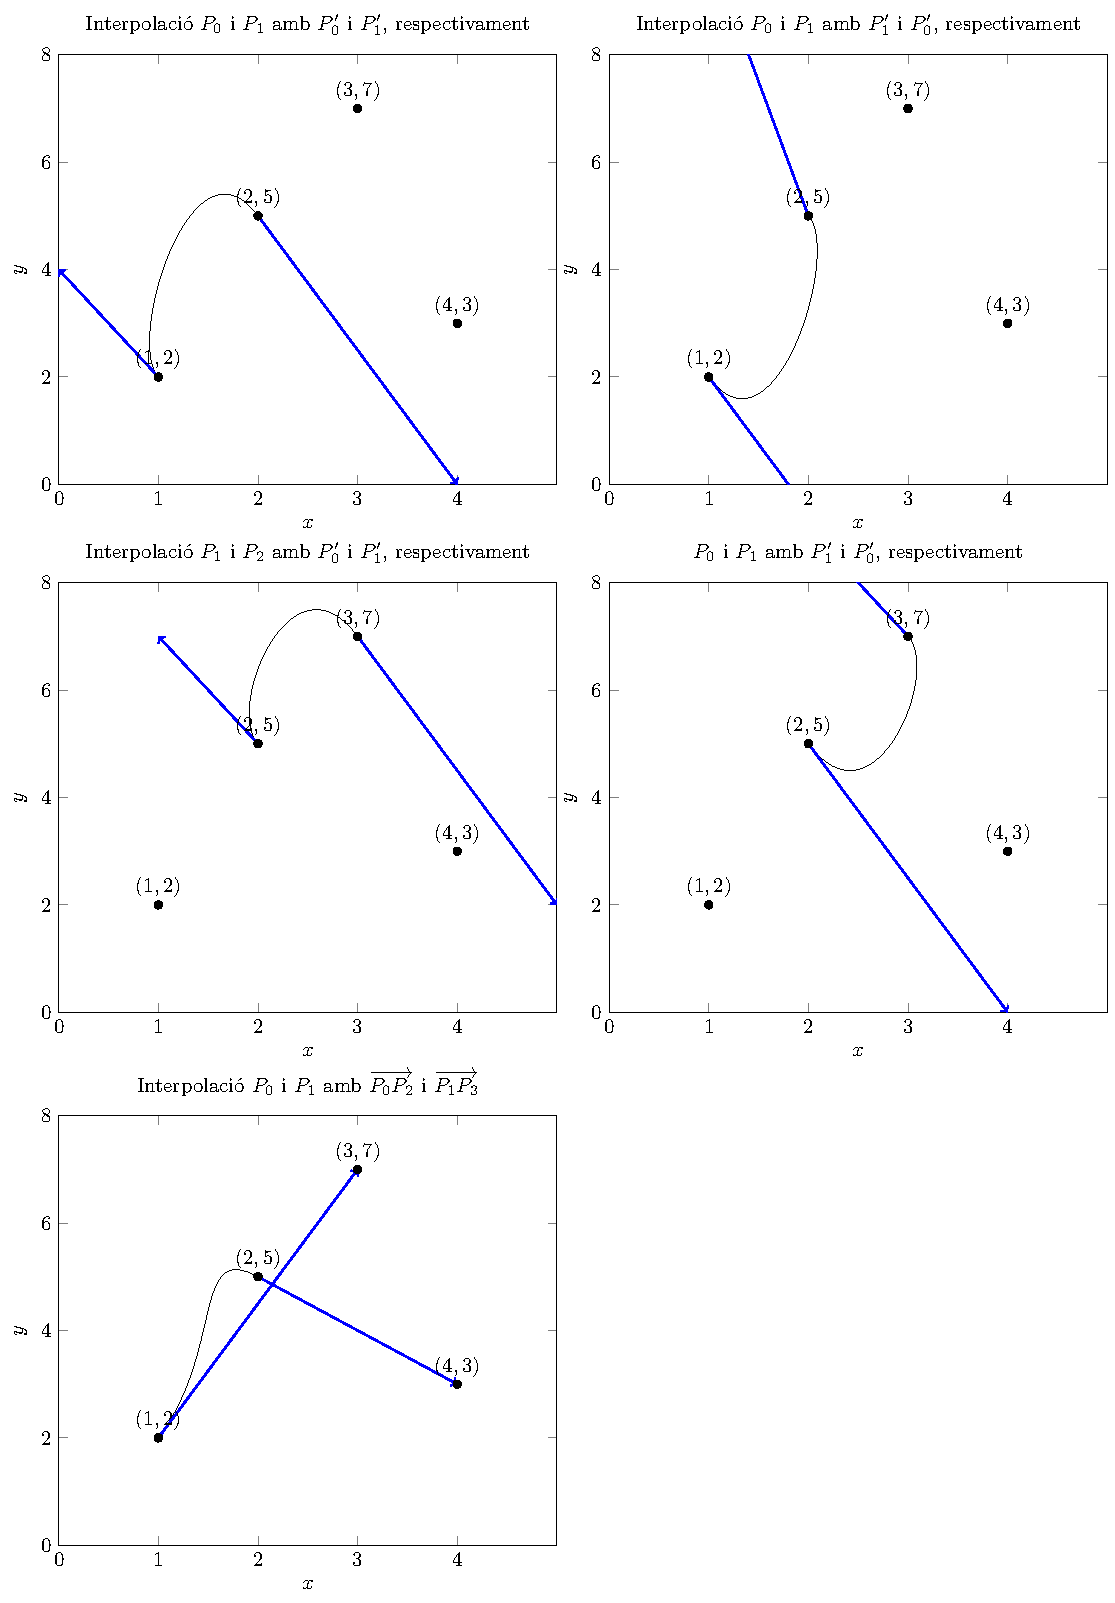
\includegraphics[width=\textwidth]{../figures/interpolaciohermite.pdf}
  \captionof{figure}{Gràfic resum de les interpolacions cúbiques d'Hermite de l'exercici.}
  \label{fig:interpolaciohermite}
\end{minipage}

\item Doneu l'spline cúbic de Béziers que passa pels punts donats (els resultats globals són graficats a la Figura \ref{fig:interpolaciobeziers}). El polinomi de Béziers per a una interpolació cúbica es construeix fent $Q_0(t)=T\cdot M \cdot G$ on:
\begin{eqnarray*}
  T&=& \begin{pmatrix}t^3 & t^2 & t & 1\end{pmatrix}\\
  M&=& \begin{pmatrix}
              -1 & 3 & -3 & 1 \\
              3 & -6 & 3 & 0 \\
              -3 & 3 & 0 & 0 \\
              1 & 0 & 0 & 0
        \end{pmatrix}\\
  G&=& \begin{pmatrix}
              P_0 \\
              P_1 \\
              P_2 \\
              P_3
        \end{pmatrix}\\
\end{eqnarray*}

o bé:
\[
  Q_0(t)=(-t^3+3t^2-3t+1)P_0+(3t^3-6t^2+3t)P_1+(-3t^3+3t^2)P_2+t^3P_3
\]

\begin{enumerate}
  \item Passa per $P_0$ i $P_3$ amb punts de control $P_1$ i $P_2$


  \[
    Q_0(t)=\begin{pmatrix}x(t)\\y(t)\end{pmatrix}=(-t^3+3t^2-3t+1)\begin{pmatrix}1\\2\end{pmatrix}
          +(3t^3-6t^2+3t)\begin{pmatrix}2\\5\end{pmatrix}
          +(-3t^3+3t^2)\begin{pmatrix}3\\7\end{pmatrix}
          +t^3\begin{pmatrix}4\\3\end{pmatrix}
  \]
  o bé
  \begin{eqnarray*}
    x(t)&=&(-t^3+3t^2-3t+1)+2(3t^3-6t^2+3t)+3(-3t^3+3t^2)+4t^3\\
    y(t)&=&2(-t^3+3t^2-3t+1)+5(3t^3-6t^2+3t)+7(-3t^3+3t^2)+3t^3
  \end{eqnarray*}
  Simplificant, obtenim:
  \begin{eqnarray*}
    x(t)&=&3t+1\\
    y(t)&=&-5t^3-3t^2+9t+2
  \end{eqnarray*}


  \blacksquare

  \item Passa per $P_0$ i $P_2$ amb punts de control $P_1$ i $P_3$


      \[
        Q_0(t)=\begin{pmatrix}x(t)\\y(t)\end{pmatrix}=(-t^3+3t^2-3t+1)\begin{pmatrix}1\\2\end{pmatrix}
              +(3t^3-6t^2+3t)\begin{pmatrix}2\\5\end{pmatrix}
              +(-3t^3+3t^2)\begin{pmatrix}4\\3\end{pmatrix}
              +t^3\begin{pmatrix}3\\7\end{pmatrix}
      \]
      o bé
      \begin{eqnarray*}
        x(t)&=&(-t^3+3t^2-3t+1)+2(3t^3-6t^2+3t)+4(-3t^3+3t^2)+3t^3\\
        y(t)&=&2(-t^3+3t^2-3t+1)+5(3t^3-6t^2+3t)+3(-3t^3+3t^2)+7t^3
      \end{eqnarray*}
      Simplificant, obtenim:
      \begin{eqnarray*}
        x(t)&=&-4t^3+3t^2+3t+1\\
        y(t)&=&11t^3-15t^2+9t+2
      \end{eqnarray*}
      \blacksquare

  \item Passa per $P_2$ i $P_3$ amb punts de control $P_0$ i $P_1$

          \[
            Q_0(t)=\begin{pmatrix}x(t)\\y(t)\end{pmatrix}=(-t^3+3t^2-3t+1)\begin{pmatrix}3\\7\end{pmatrix}
                  +(3t^3-6t^2+3t)\begin{pmatrix}1\\2\end{pmatrix}
                  +(-3t^3+3t^2)\begin{pmatrix}2\\5\end{pmatrix}
                  +t^3\begin{pmatrix}4\\3\end{pmatrix}
          \]
          o bé
          \begin{eqnarray*}
            x(t)&=&3(-t^3+3t^2-3t+1)+1(3t^3-6t^2+3t)+2(-3t^3+3t^2)+4t^3\\
            y(t)&=&7(-t^3+3t^2-3t+1)+2(3t^3-6t^2+3t)+5(-3t^3+3t^2)+3t^3
          \end{eqnarray*}
          Simplificant, obtenim:
          \begin{eqnarray*}
            x(t)&=&-2t^3+9t^2-6t+3\\
            y(t)&=&-13t^3+24t^2-15t+2
          \end{eqnarray*}
          \blacksquare

  \item Passa per $P_1$ i $P_2$ amb punts de control $P_0$ i $P_3$


  \[
    Q_0(t)=\begin{pmatrix}x(t)\\y(t)\end{pmatrix}=(-t^3+3t^2-3t+1)\begin{pmatrix}2\\5\end{pmatrix}
          +(3t^3-6t^2+3t)\begin{pmatrix}1\\2\end{pmatrix}
          +(-3t^3+3t^2)\begin{pmatrix}4\\3\end{pmatrix}
          +t^3\begin{pmatrix}3\\7\end{pmatrix}
  \]
  o bé
  \begin{eqnarray*}
    x(t)&=&2(-t^3+3t^2-3t+1)+1(3t^3-6t^2+3t)+4(-3t^3+3t^2)+3t^3\\
    y(t)&=&5(-t^3+3t^2-3t+1)+2(3t^3-6t^2+3t)+3(-3t^3+3t^2)+7t^3
  \end{eqnarray*}
  Simplificant, obtenim:
  \begin{eqnarray*}
    x(t)&=&-8t^3+12t^2-3t+2\\
    y(t)&=&-t^3+12t^2-9t+5
  \end{eqnarray*}
\blacksquare


\end{enumerate}

\begin{minipage}[t]{\linewidth}
  \vspace{-2ex}
  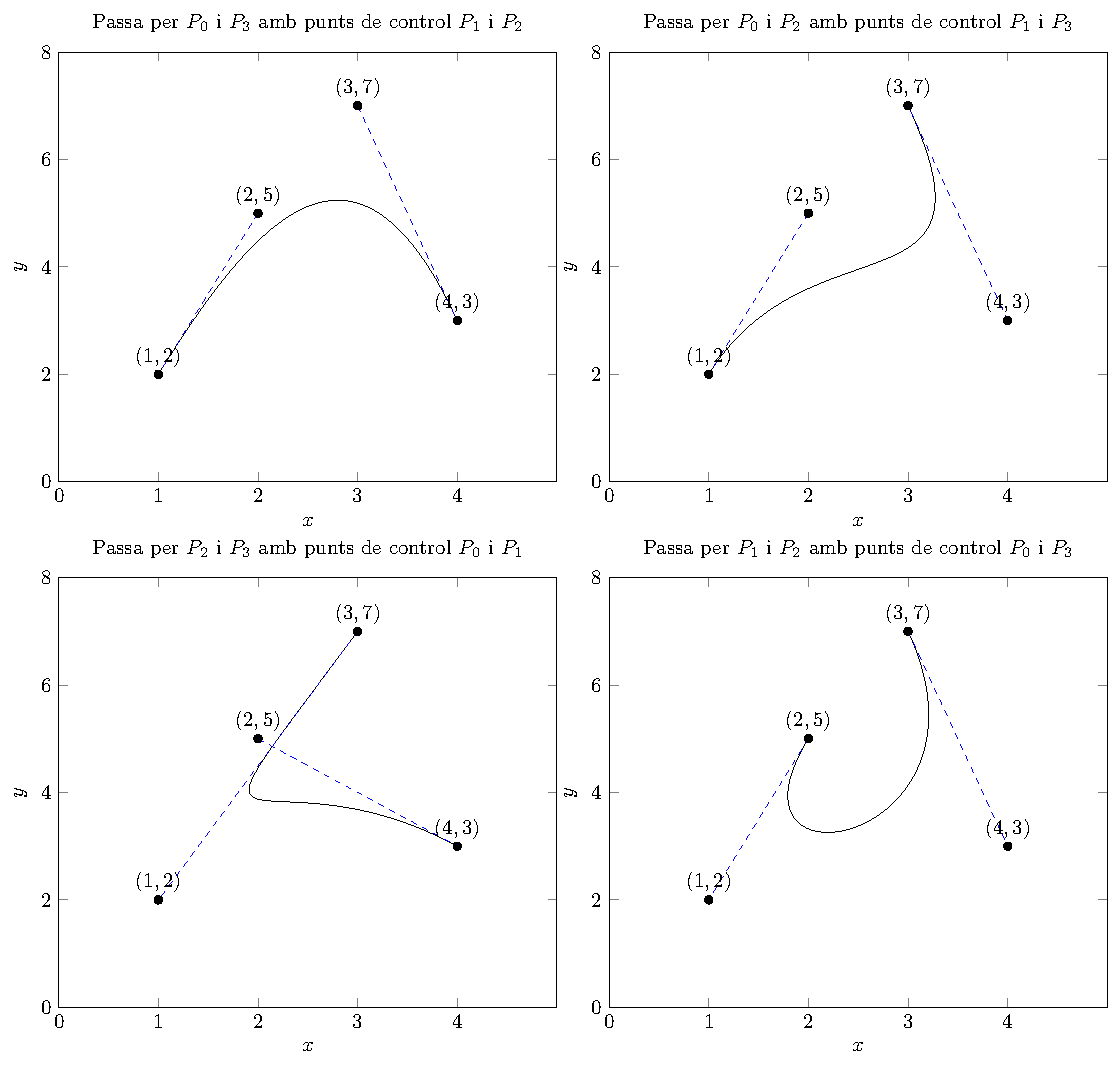
\includegraphics[width=\textwidth]{../figures/interpolaciobeziers.pdf}
  \captionof{figure}{Gràfic resum de les interpolacions cúbiques de Béziers de l'exercici.}
  \label{fig:interpolaciobeziers}
\end{minipage}
Un exemple de codi MATLAB per generar les interpolacions de Beziers pot ser:
\lstinputlisting{../code/polinomisBeziers.m}

\end{enumerate}

\Exercise Donades les bases de $\mathbb{R}^2$, $B=\{(1,-2),(0,1)\}$ i $D=\{(3,2),(-1,1)\}$:
\begin{enumerate}[label=(\alph*)]
  \item Doneu la matriu de canvi de base de $B$ a $C$ (base canònica)
  \item Doneu la matriu de canvi de base de $C$ a $B$
  \item Doneu la matriu de canvi de base de $D$ a $B$
\end{enumerate}

\Answer Només cal recordar que la matriu de canvi de base de $B$ a $C$ és la matriu dels vectors de la base $B$ en funció de la base $C$, i que la matriu del canvi oposat és la inversa de l'anterior:
\begin{enumerate}[label=(\alph*)]
  \item Doneu la matriu de canvi de base de $B$ a $C$ (base canònica)
  \[
    A_{B\rightarrow C} = \begin{pmatrix}1&0\\-2&1\end{pmatrix}
  \]
  \blacksquare

  \item Doneu la matriu de canvi de base de $C$ a $B$
  \[
    A_{C\rightarrow B} = (A_{B\rightarrow C})^{-1} =\begin{pmatrix}1&0\\-2&1\end{pmatrix}^{-1}
  \]
  I obtenim la inversa fent:
  \[
    \begin{pmatrix}1&0& \vrule &1&0 \\-2&1& \vrule &0&1\end{pmatrix} \approx
    \begin{pmatrix}1&0& \vrule &1&0 \\0&1& \vrule &2&1\end{pmatrix}
  \]
  Per tant,
  \[
    A_{C\rightarrow B} = \begin{pmatrix}1&0\\2&1\end{pmatrix}
  \]
  \blacksquare

  \item Doneu la matriu de canvi de base de $D$ a $B$
  Podem construir-la amb una composició de transformacions lineals, és a dir, amb una multiplicació de les matrius que les defineixen:
  \begin{eqnarray*}
    A_{D\rightarrow B} &=& A_{C\rightarrow B}\cdot A_{D\rightarrow C}\\
    A_{D\rightarrow B} &=& \begin{pmatrix}1&0\\2&1\end{pmatrix} \cdot
    \begin{pmatrix}3&-1\\2&1\end{pmatrix}=
    \begin{pmatrix}3&-1\\8&-1\end{pmatrix}
  \end{eqnarray*}
  \blacksquare

\end{enumerate}

\Exercise El vector $\overrightarrow{PQ}=(-4,8)$ té l'origen en el punt $P(6,-1)$. Determina les coordinades de l'extrem $Q$ i el mòdul d'aquest vector.

\Answer

Podem expressar el vector $\overrightarrow{PQ}$ com la diferència dels vectors que identifiquen els seus dos extrems:

\begin{minipage}{0.49\linewidth}
  \[\overrightarrow{PQ}=Q-P\]
\begin{eqnarray*}
  (-4,8)&=&Q-(6,-1)\\
  (-4,8)+(6,-1)&=&Q\\
  (2,7)&=&Q
\end{eqnarray*}
Pel que fa al mòdul:
\[\abs{\overrightarrow{PQ}}=\sqrt{(-4)^2+8^2}=\sqrt{80}=4\sqrt{5}\]
\end{minipage}
\hspace{0.01\linewidth}
\begin{minipage}{0.49\linewidth}
\begin{center}
  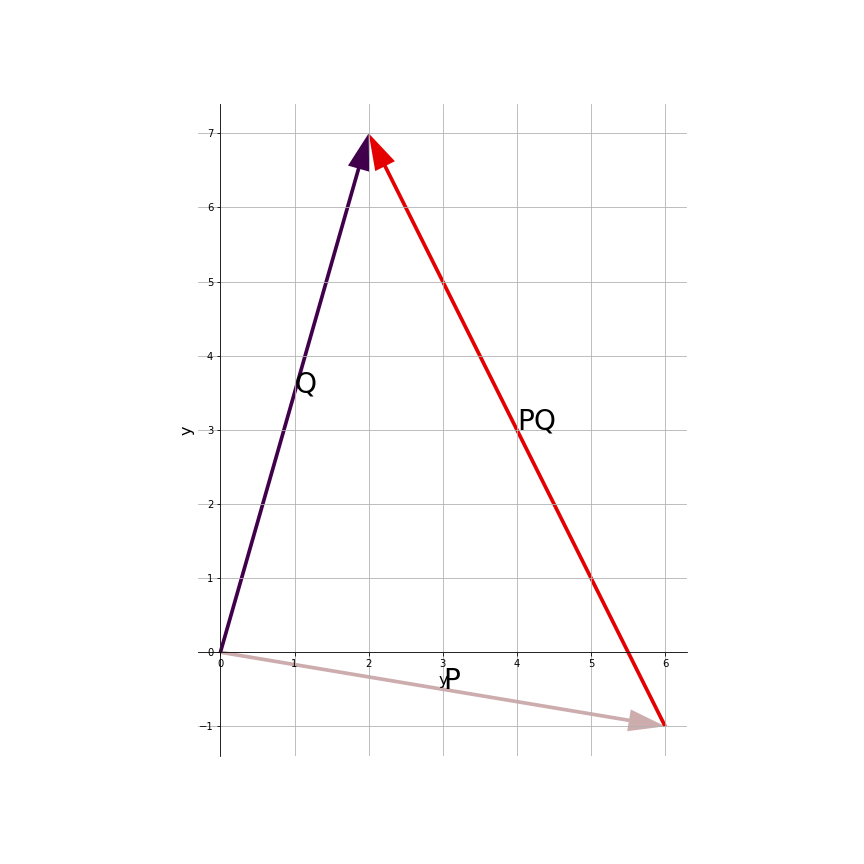
\includegraphics[scale=0.3]{vectorPQ}
\end{center}
\end{minipage}


\blacksquare 
\Exercise El vector $\overrightarrow{PQ}=(3,-6)$ té l'extrem en el punt $Q(2,1)$. Determina les coordenades de l'origen $P$ i el mòdul d'aquest vector.

\Answer

Podem expressar el vector $\overrightarrow{PQ}$ com la diferència dels vectors que identifiquen els seus dos extrems:

\begin{minipage}{0.49\linewidth}
\[\overrightarrow{PQ}=Q-P\]
\begin{eqnarray*}
  (3,-6)&=&(2,1)-P\\
  P=&=&(2,1)-(3,-6)\\
  P&=&(-1,7)
\end{eqnarray*}
Pel que fa al mòdul:
\[\abs{\overrightarrow{PQ}}=\sqrt{3^2+(-6)^2}=\sqrt{45}=3\sqrt{5}\]
\end{minipage}
\hspace{0.01\linewidth}
\begin{minipage}{0.49\linewidth}
\begin{center}
  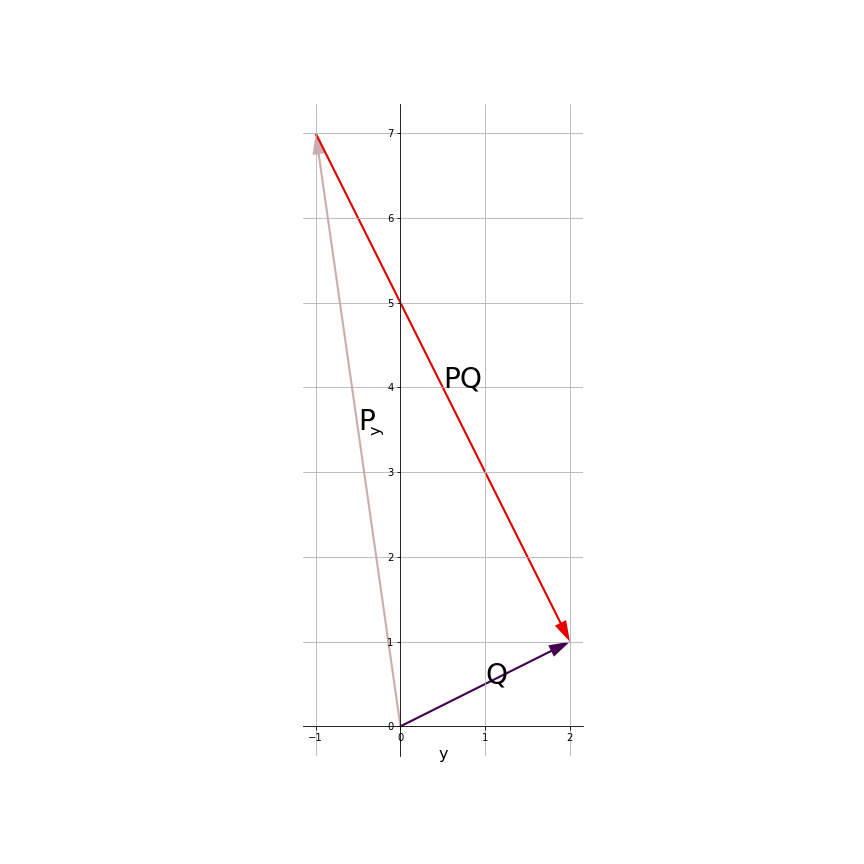
\includegraphics[scale=0.3]{vectorPQ2}
\end{center}
\end{minipage}


\blacksquare 
\Exercise  
A partir de la definició d'espai vectorial, qui són $\vec{e}$ (a $\mathbb{R}^2$) i $e$? Passa el mateix a $\mathbb{R}$ o $\mathbb{R}^3$? I a $\mathbb{R}^n$?

\Answer

$\vec{e}$ és l'element neutre de la suma de vectors tal que $\vec{u}+\vec{e}=\vec{u}$. Per a qualsevol vector $\vec{u} \in \mathbb{R}^2$:
\[(u_1,u_2)+(e_1,e_2)=(u_1,u_2) \Rightarrow (e_1,e_2)=(0,0)\]
A $\mathbb{R}^3$? I a $\mathbb{R}^n$ seria, respectivament, $(0,0,0)$ i $(0,\ldots ,0)\in\mathbb{R}^n $.

Respecte el valor de l'element neutre $e \in \mathbb{R}$ tal que $e \cdot \vec{u} = \vec{u}$, si agafem per exemple $\vec{u}\in \mathbb{R}^2$:
\[e \cdot (u_1,u_2) = (e\cdot u_1,e\cdot u_2)= (u_1,u_2) \Rightarrow e=1\]

i el mateix succeeix per a un espai vectorial d'$\mathbb{R}^3$ i $\mathbb{R}^n$.

\blacksquare 
\Exercise  
Calcula la norma del vector d'$\mathbb{R}^5$ $\vec{u}=(1,-2,-3,0,2)$.

\Answer

La norma del vector $\vec{u}$ serà:
\[\norm{\vec{u}}=\sqrt{1^2+(-2)^2+(-3)^2+0^2+2^2}=\sqrt{18}=3\sqrt{2}\]
\blacksquare 
\Exercise Donats els punts $A(1,1)$, $B=(0,-1)$ i el vector $\vec{u}=(2,4)$
\begin{enumerate}
  \item Calcula els vectors que van des de l'origen de coordenades cap a cadascun dels punts $A$ i $B$ (pregunta trampa...).
  \item Calcula i dibuixa $\overrightarrow{AB}$.
  \item Calcula i dibuixa $\overrightarrow{BA}$.
  \item Si $\vec{u}=\overrightarrow{AC}$, quina posició és $C$?
  \item Si $\vec{u}=\overrightarrow{CB}$, quina posició és $C$?
  \item Dóna una altres dos punts $A$ i $B$ que tinguin el mateix vector desplaçament $\overrightarrow{AB}$.
\end{enumerate} 

\Answer
\begin{enumerate}
  \item Calcula els vectors que van des de l'origen de coordenades cap a cadascun dels punts $A$ i $B$ (pregunta trampa...). El vector el trobarem substraient el punt inicial (en aquest cas $O=(0,0)$) del punt final
    \begin{itemize}
      \item \[\overrightarrow{OA}=A-O=(1,1)\]
      \item \[\overrightarrow{OB}=B-O=(0,-1)\]
    \end{itemize}
  \item Calcula i dibuixa $\overrightarrow{AB}$. 
    \[\overrightarrow{AB}=B-A=(0,-1)-(1,1)=(-1,-2)\]
    \begin{center}
      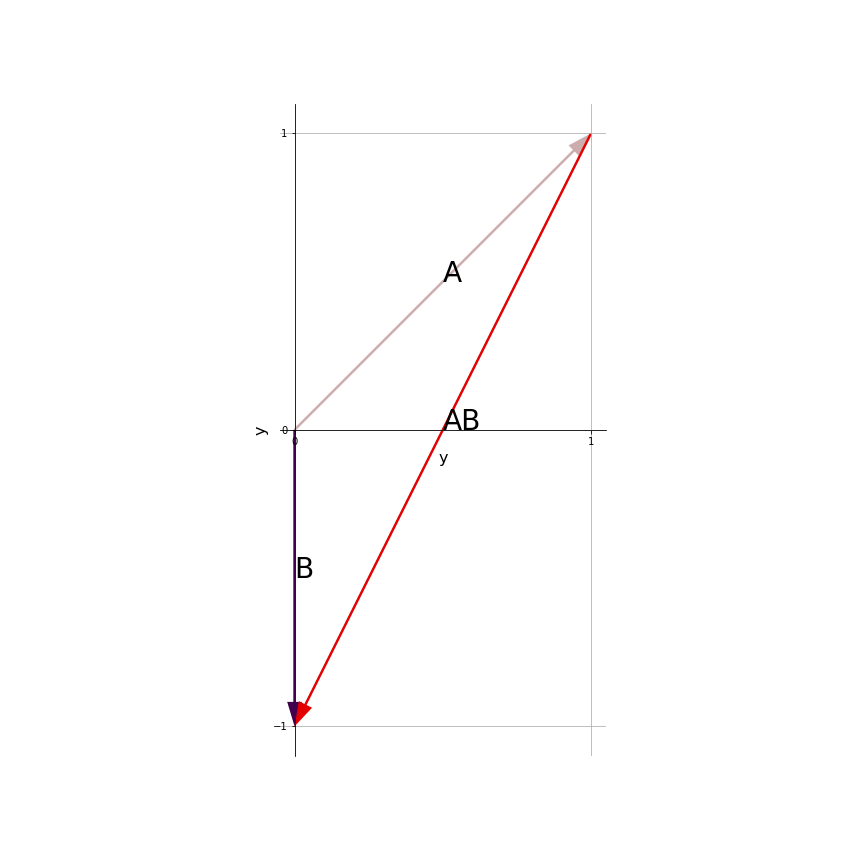
\includegraphics[scale=0.3]{vectorAB}
   \end{center}
  \item Calcula i dibuixa $\overrightarrow{BA}$.
    \[\overrightarrow{BA}=A-B=(1,1)-(0,-1)=(1,2)\]
    \begin{center}
      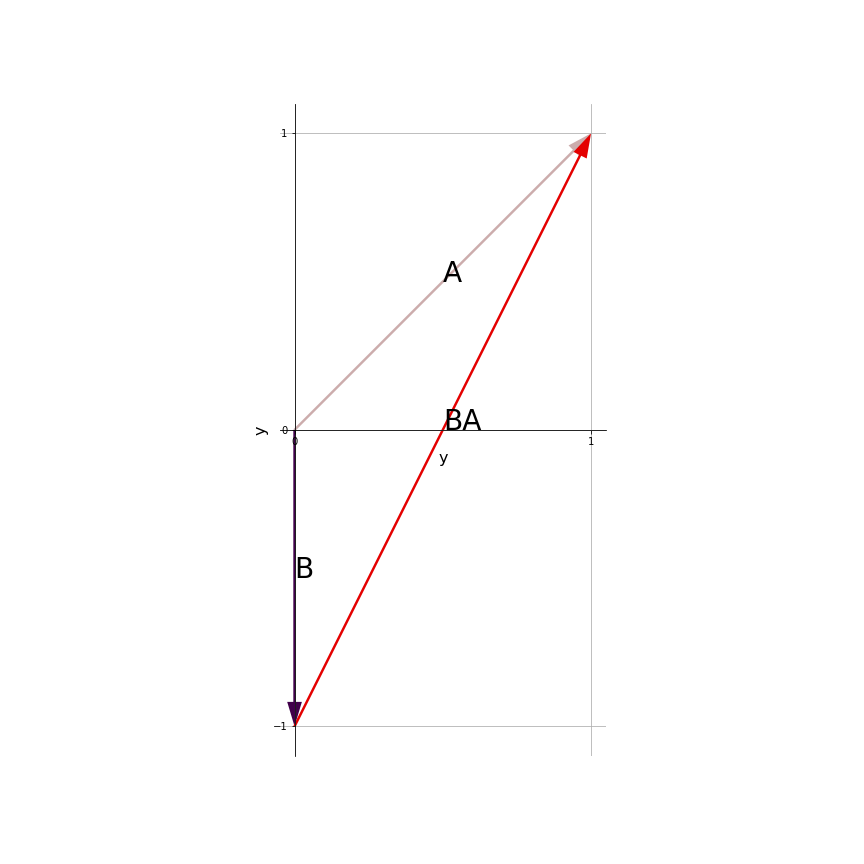
\includegraphics[scale=0.3]{vectorBA}
    \end{center}
  \item Si $\vec{u}=\overrightarrow{AC}$, quina posició és $C$?
  \[\vec{u}=\overrightarrow{AC} = C-A \Rightarrow C=A+\vec{u}=(1,1)+(2,4)=(3,5)\]
  \begin{center}
    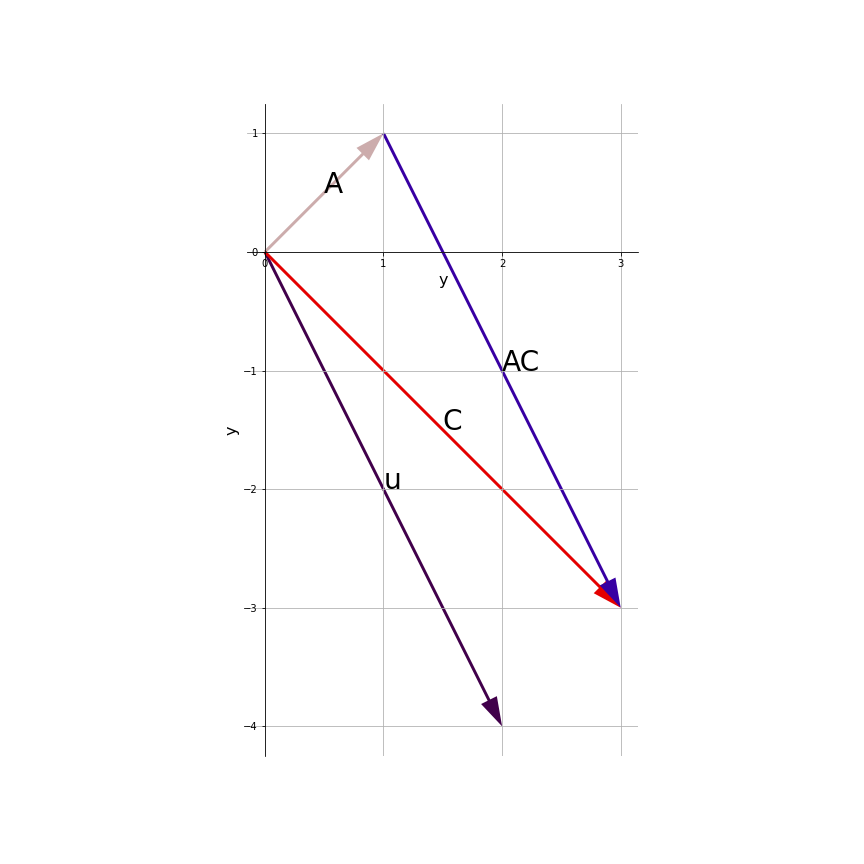
\includegraphics[scale=0.3]{vectorC1}
  \end{center}
  \item Si $\vec{u}=\overrightarrow{CB}$, quina posició és $C$?
  \item   \[\vec{u}=\overrightarrow{CB} = B-C \Rightarrow C=B-\vec{u}=(0,-1)-(1,1)=(-1,-2)\]
  \begin{center}
    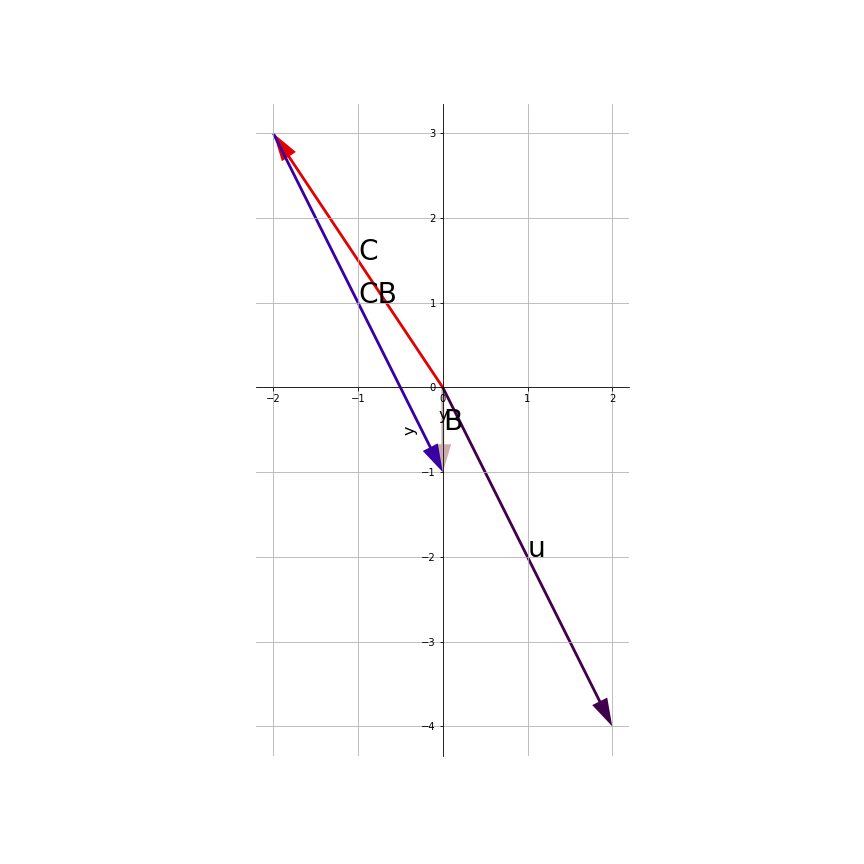
\includegraphics[scale=0.3]{vectorC2}
  \end{center}

  \item Dóna una altres dos punts $A$ i $B$ que tinguin el mateix vector desplaçament $\overrightarrow{AB}$.
  Només cal agafar un punt $D$ qualsevol i sumar-li el vector $\overrightarrow{AB}$ per trobar el punt $E$. Alguns exemples
  \begin{center}
    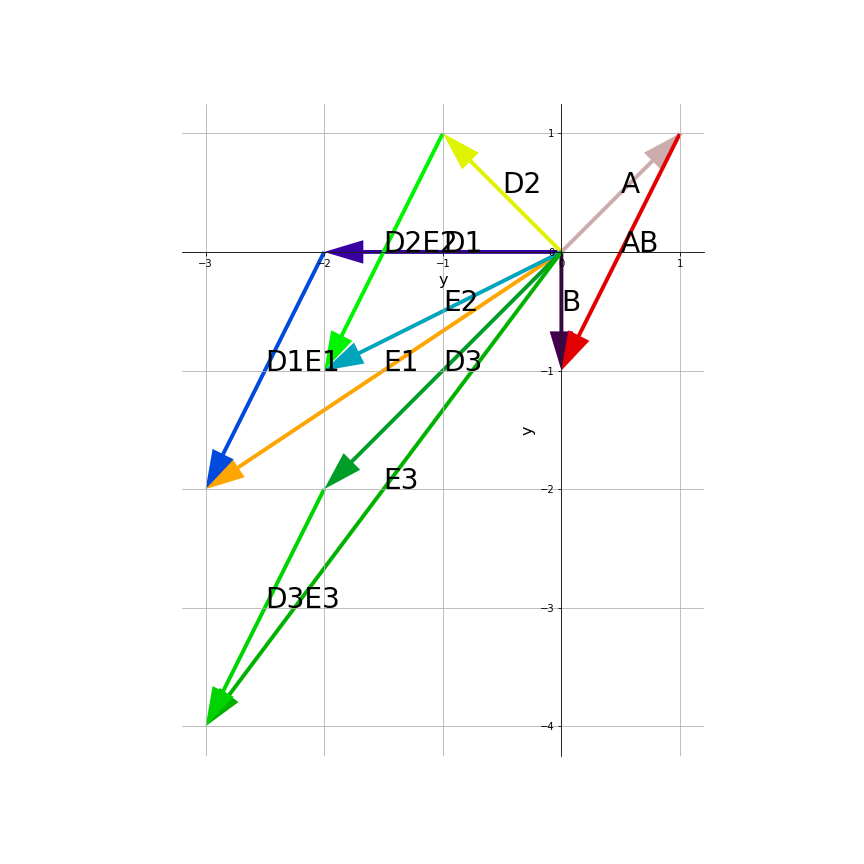
\includegraphics[scale=0.3]{vectorDE}
  \end{center}

\end{enumerate}
\blacksquare 

  \Exercise Siguin $\uvec{u}=(2,-1)$ i $\uvec{v}=(3,4)$, es demana el següent:
  \begin{enumerate}
    \item Efectueu les següents operacions:
    \begin{enumerate}
      \item $\uvec{u}+\uvec{v}$
      \item $2\uvec{u}+3\uvec{v}$
      \item $\uvec{u}-\frac{2}{3}\uvec{v}$
    \end{enumerate}
    \item Calculeu $\uvec{u}\cdot \uvec{v}$
    \item Determineu $\norm{\uvec{u}}$ i $\norm{\uvec{v}}$
    \item Trobeu l'angle format pels dos vectors
  \end{enumerate}

  \Answer Seguint l'ordre de les qüestions plantejades:
  \begin{enumerate}
    \item Fem les operacions:
    \begin{enumerate}
      \item $\uvec{u}+\uvec{v}=(2,-1)+(3,4)=(5,3)$
      \item $2\uvec{u}+3\uvec{v}=2(2,-1)+3(3,4)=(4,-2)+(9,12)=(13,10)$
      \item $\uvec{u}-\frac{2}{3}\uvec{v}=(2,-1)-\frac{2}{3}(3,4)=(2,-1)-(2,\frac{8}{3})=(0,-\frac{11}{3})$
    \end{enumerate}
    \item $\uvec{u}\cdot \uvec{v}=(2,-1)\cdot(3,4)=2\cdot3+(-1)\cdot4=6-4=2$
    \item $\norm{\uvec{u}}=\sqrt{2^2+(-1)^2}=\sqrt{5}$; $\norm{\uvec{v}}=\sqrt{3^2+4^2}=\sqrt{25}=5$
    \item L'angle format pels dos vectors es pot obtenir usant:
    \[\cos{\alpha}=\frac{\uvec{u}\cdot \uvec{v}}{\norm{\uvec{u}} \cdot \norm{\uvec{v}}}=\frac{2}{5\sqrt{5}}
    \]
    que correspon a un angle de 1.39 radiants, o bé 79.69\degree.
  \end{enumerate}
  \blacksquare

\Exercise Determinar si els vectors $\uvec{u}$ i $\uvec{v}$ són paral·lels, ortogonals o cap de les dues coses:

\begin{enumerate}
  \item $\uvec{u}=(1,-2)$ i $\uvec{v}=(2.-4)$
  \item $\uvec{u}=(1,-2,1)$ i $\uvec{v}=(2,1,0)$
  \item $\uvec{u}=\uvec{j}+6\uvec{k}$, $\uvec{v}=\uvec{i}-2\uvec{j}-\uvec{k}$
\end{enumerate}

\Answer Per determinar el paral·lelisme, observem si un dels dos vectors és proporcional a l'altre. Per determinar l'ortogonalitat en fem el producte escalar:

\begin{enumerate}
  \item $\uvec{u}=(1,-2)$ i $\uvec{v}=(2,-4)$. Veiem que $\uvec{v}=2\uvec{u}$ i, per tant, són paral·lels.
  \item $\uvec{u}=(1,-2,1)$ i $\uvec{v}=(2,1,0)$. No són paral·lels perquè no són proporcionals. Per saber si són ortogonals en calculem el producte escalar: $\uvec{u}\cdot\uvec{v}=1\cdot2+(-2)\cdot1+1\cdot0=0$. Per tant, són dos vectors ortogonals.
  \item $\uvec{u}=\uvec{j}+6\uvec{k}$, $\uvec{v}=\uvec{i}-2\uvec{j}-\uvec{k}$. Novament no són proporcionals i, per tant, no són paral·lels. Pel que fa al producte escalar: $\uvec{u}\cdot\uvec{v}=0\cdot1+1\cdot(-2)+6\cdot(-1)=-8\neq0$. Per tant, no són ni paral·lels ni ortogonals.
\end{enumerate}
\blacksquare

\Exercise Expressa en forma polar cadascun dels punts següents:

\begin{multicols}{2}
  \begin{enumerate}
    \item $(3,3)$  \item $(-\sqrt{3},3)$ \item $(-\sqrt{8},-\sqrt{8})$ \item $(6,-8)$
  \end{enumerate}
\end{multicols}

\Answer

D'acord amb la imatge, el canvi de coordenades cartesianes a polars ve donada per:


\begin{minipage}{0.49\linewidth}
  \begin{center}  
    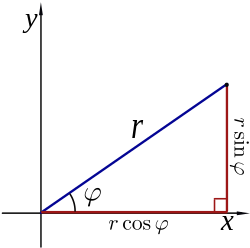
\includegraphics[scale=0.5]{polar_fig}
  \end{center}
\end{minipage}
\hspace{0.01\linewidth}
\begin{minipage}{0.49\linewidth}
  \[\begin{cases}r=\sqrt{x^2+y^2}\\ \varphi=\atan{\frac{y}{x}}\end{cases}\]
\end{minipage}
Per tant:
\begin{enumerate}
  \item \[\begin{cases}r=\sqrt{3^2+3^2}=3\sqrt{2}\\\varphi=\atan{1}=\frac{\pi}{4}\end{cases}\]  
  \item  \[\begin{cases}r=\sqrt{{-\sqrt{3}}^2+3^2}=2\sqrt{3}\\\varphi=\atan{-\frac{3}{\sqrt{3}}}=\frac{2\pi}{3}\end{cases}\]  
  \item \[\begin{cases}r=\sqrt{-\sqrt{8}^2+-\sqrt{8}^2}=4\\\varphi=\atan{\frac{-\sqrt{8}}{-\sqrt{8}}}=-\frac{5\pi}{4}\end{cases}\]  
  \item \[\begin{cases}r=\sqrt{6^2+(-8)^2}=10\\\varphi=\atan{\frac{-8}{6}}=2.21\, \mathrm{rad}\end{cases}\]  
\end{enumerate}
\begin{center}
  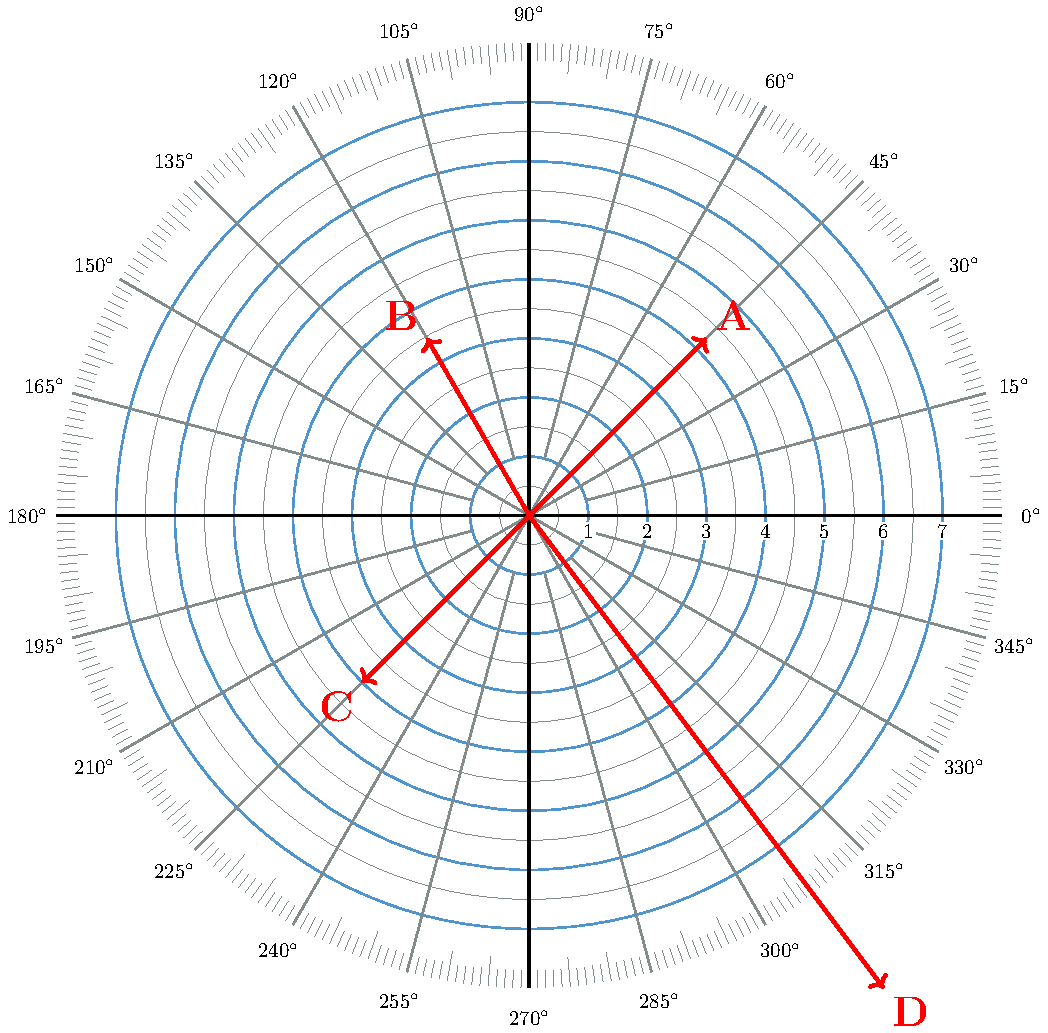
\includegraphics[scale=0.6]{polar1}
\end{center}

\blacksquare 
\Exercise Determineu la posició relativa dels plans següents
\begin{enumerate}
  \item $x-y+z=1$ i $2x+2y-3z=4$
  \item $4x+2y+6z=12$ i $3x+6y+2z=6$
\end{enumerate}

\Answer Només cal resoldre els sistemes d'equacions resultants d'aplegar-los i comprovar si són compatibles o incompatibles.
\begin{enumerate}[label=\alph*) ]
  \item $x-y+z=1$ i $2x+2y-3z=4$

\[
\begin{cases}
  x-y+z=1\\
  2x+2y-3z=4
\end{cases}
\]

Aplicant l'eliminació de Gauss-Jordan:

\begin{elimination}[3]{3}{1.1em}{1.1}% Decreased from 1.75em
      \eliminationstep
      {
          1 & -1 & 1 & 1  \\
          2 & 2 & -3 & 4
      }
      {
          \\
          -2 R_{1}\\
      }
      \eliminationstep
      {
      1 & -1 & 1 & 1  \\
      0 & 4 & -5 & 2
  }
  {
      \\
      \\
  }
\end{elimination}

Es comprova que $rg(A)=2$ i $rg(A|B)=2$ i, per tant, el sistema és compatible indeterminat de rang 2. Els plans es tallen en una recta.
\blacksquare

  \item $4x+2y+6z=12$ i $3x+6y+2z=6$


  \[
  \begin{cases}
    4x+2y+6z=12\\
    3x+6y+2z=6
  \end{cases}
  \]

  Aplicant l'eliminació de Gauss-Jordan:

  \begin{elimination}[3]{3}{1.1em}{1.1}% Decreased from 1.75em
        \eliminationstep
        {
            4 & 2 & 6 & 12  \\
            3 & 6 & 2 & 6
        }
        {
            \\
            -\frac{3}{4} R_{1}\\
        }
        \eliminationstep
        {
        4 & 2 & 6 & 12  \\
        0 & \frac{9}{2} & -\frac{5}{2} & -3
    }
    {
        \\
        \\
    }
  \end{elimination}

  Es comprova que $rg(A)=2$ i $rg(A|B)=2$ i, per tant, el sistema és compatible indeterminat de rang 2. Els plans es tallen en una recta.
  \blacksquare

\end{enumerate}

\Exercise Determineu la posició relativa de les rectes següents:

\begin{enumerate}
  \item $\begin{cases}x=4t+2\\y=3\\z=-t+1\end{cases}$ i $\begin{cases}x=2s+2\\y=2s+3\\z=s+1\end{cases}$
  \item $\begin{cases}x+3y=6\\y-z=0\end{cases}$ i $\frac{x-1}{4}=y+2=\frac{z+3}{-3}$
\end{enumerate}

\Answer D'entrada mirem si són paral·leles (o coincidents) especte si es creuen (o es tallen) analitzant els seus vectors directors. Després mirarem si realemnt coincideixen an algun o infinits punts o no.

\begin{enumerate}
  \item $\begin{cases}x=4t+2\\y=3\\z=-t+1\end{cases}$ i $\begin{cases}x=2s+2\\y=2s+3\\z=s+1\end{cases}$

En aquest cas, els dos vectors directors són $\uvec{u}=(4,0-1)$ i $\uvec{v}=(2,2,1)$, amb la qual cosa veiem que no són paral·leles (ni coincidents). Per saber si es tallen hem d'assegurar que passin per algun punt comú. Així, si el sistema
\[
\begin{cases}4t+2=2s+2\\3=2s+3\\-t+1=s+1\end{cases}
\]
és compatible, també ho serà determinat, per força. És fàcil veure que el sistema es soluciona per a $s=t=0$. Per tant, les dues rectes es tallen, justament, en el punt que determinen aquests dos paràmetres: $P=(2,3,1)$, cosa que es podia observar directament a partir de les equacions paramètriques de l'enunciat.
\blacksquare

  \item $\begin{cases}x+3y=6\\y-z=0\end{cases}$ i $\frac{x-1}{4}=y+2=\frac{z+3}{-3}$

En aquest podem analitzar directament el sistema d'equacions format per totes les equacions donades:

\[
\begin{cases}
  x+3y=6\\
  y-z=0\\
  x-1=4y+8\\
  -3y-6=z+3
\end{cases}
\]
arranjant una mica:
\[
\begin{cases}
  x+3y=6\\
  0x+y-z=0\\
  x-4y+0z=9\\
  0x-3y-z=9
\end{cases}
\]

D'on podem analitzar els rangs de la matriu de coeficients i de la matriu ampliada $(A|B)$ usant, per exemple, el mètode de Gauss-Jordan:

\begin{elimination}[3]{3}{1.1em}{1.1}% Decreased from 1.75em
    \eliminationstep
    {
        1 & 3 & 0 & 6  \\
        0 & 1 & -1 & 0  \\
        1 & -4 & 0 & 9  \\
        0 & -3 & -1 & 9
    }
    {
        \\
        \\
        -R_{1}\\
        \\
    }
    \eliminationstep
    {
    1 & 3 & 0 & 6  \\
    0 & 1 & -1 & 0  \\
    0 & 7 & 0 & -3  \\
    0 & -3 & -1 & 9
    }
    {
        \\
        \\
        -7R_{2}\\
        +3R_{2}
    }
    \\
    \eliminationstep
    {
    1 & 3 & 0 & 6  \\
    0 & 1 & -1 & 0  \\
    0 & 0 & 7 & -3  \\
    0 & 0 & -4 & 9
    }
    {
        \\
        \\
        \frac{1}{7} R_{3}\\
        -\frac{1}{4} R_{4}
    }
    \eliminationstep
    {
    1 & 3 & 0 & 6  \\
    0 & 1 & -1 & 0  \\
    0 & 0 & 1 & -\frac{3}{7}  \\
    0 & 0 & 1 & -\frac{9}{4}
    }
    {
        \\
        \\
        \\
        -R_{3}\\
    }
    \\
    \eliminationstep
    {
    1 & 3 & 0 & 6  \\
    0 & 1 & -1 & 0  \\
    0 & 0 & 1 & -\frac{3}{7}  \\
    0 & 0 & 0 & -\frac{51}{28}
    }
    {
        \\
        \\
        \\
        \\
    }
\end{elimination}

d'on deduïm que el sistema és incompatible. Per tant, les rectes no es toquen. Per saber si són paral·leles podem mirar també el resultat de l'eliminació de Gauss-Jordan. Finalment obtenim tres línies de la matriu (les tres primeres) que representen un sistema equvalent al creuament de tres plans en un sol punt. Per tant, les des rectes es creuen en l'espai i no són paral·leles. En aquest darrer cas hauríem obtingut només dues files de la matriu $A$ linealment independents.



\end{enumerate}

\Exercise Calcula $\begin{pmatrix}1&1\\3&-1\end{pmatrix}^6$ usant el concepte de valors i vectors propis de la matriu.

\Answer
Sabem que si una matriu $A$ és diagonalitzable, podem expressar-la com
\[D=P^{-1}AP\]
on $D$ és una matriu diagonal amb els valors propis de la matriu $A$ i $P$ és una matriu quines columnes representen els vectors propis associats a cada valor propi.

Si usem aquesta expressió, fer l'operació és senzilla. Efectivament:
\[\left(PDP^{-1}\right)^6=A^6\]
o, el que és el mateix:
\begin{eqnarray}
  PDP^{-1}PDP^{-1} PDP^{-1} PDP^{-1}PDP^{-1}PDP^{-1}&=&A^6\nonumber\\
  PD^6P^{-1}&=&A^6\label{eq_A6}
\end{eqnarray}


Anem, doncs, a cercar els valors i vectors propis de la matriu. Aquests seran els valors que compleixin:

\[
  \begin{pmatrix}1&1\\3&-1\end{pmatrix}
  \begin{pmatrix}x\\y\end{pmatrix}=\lambda\begin{pmatrix}x\\y\end{pmatrix}\]

  Perquè això tingui solució diferent de la trivial ($(x,y)=(0,0)$) cal que el determinant secular sigui igual a zero:
  \[
  \begin{vmatrix}1-\lambda&1\\3&-1-\lambda\end{vmatrix}=0  
  \]
  Per tant, cal solucionar el polinomi característic de la matriu:
  \[(1-\lambda)(-1-\lambda)-3=0\]
  d'on $\lambda=\pm 2$.


Un cop tenim els valors propis, trobem els vectors propis que hi estan vinculats:

\begin{description}
  \item[$\boxed{\lambda_1=2}$] 
  \[
    \begin{pmatrix}1&1\\3&-1\end{pmatrix}
  \begin{pmatrix}x\\y\end{pmatrix}=2\begin{pmatrix}x\\y\end{pmatrix}
  \]
  Solucionem el sistema:
  \[
    \systeme*{x+y=2x,3x-y=2y} \Rightarrow \systeme*{-x+y=0,x-y=0} \Rightarrow x=y
  \]
  Per tant, un vector propi\footnote{De fet, el conjunt de vectors propis associats a un determinat valor propi forma un subespai vectorial.} associat a $\lambda_1=2$ és $\uvec{v}_1=\begin{pmatrix}1\\1\end{pmatrix}$. 
  \item[$\boxed{\lambda_1=-2}$] 
  \[
    \begin{pmatrix}1&1\\3&-1\end{pmatrix}
  \begin{pmatrix}x\\y\end{pmatrix}=-2\begin{pmatrix}x\\y\end{pmatrix}
  \]
  Solucionem el sistema:
  \[
    \systeme*{x+y=-2x,3x-y=-2y} \Rightarrow 3x+y=0
  \]
  Per tant, un vector propi associat a $\lambda_2=2$ és $\uvec{v}_2=\begin{pmatrix}1\\-3\end{pmatrix}$. 
\end{description}

Construïm ara l'expressió de l'Eq. \ref{eq_A6}:

\begin{eqnarray*}
A^6 &=&\begin{pmatrix}1&1\\1&-3\end{pmatrix}\begin{pmatrix}2&0\\0&-2\end{pmatrix}^6\begin{pmatrix}1&1\\1&-3\end{pmatrix}^{-1}\\
&=&\begin{pmatrix}1&1\\1&-3\end{pmatrix}\begin{pmatrix}64&0\\0&64\end{pmatrix}\begin{pmatrix}\frac{3}{4}&\frac{1}{4}\\\frac{1}{4}&-\frac{1}{4}\end{pmatrix}\\
&=&\begin{pmatrix}64&0\\0&64\end{pmatrix}
\end{eqnarray*}

Sabries dir d'on prové el fet que, en aquest cas particular, la potència de la matriu sigui idèntica a la potència de la seva matriu semblant diagonal?




\blacksquare

\Exercise
  Determineu el valor de $m$ i $p$, perquè es pugui realitzar el producte següent:
  \[
    (P^t\cdot Q^t)\cdot M^t
    \]
    si $M_{2 \times 3}$, $P_{m \times p}$, $Q_{3 \times 4}$ i el resultat del producte és una matriu quadrada.

\Answer
  Per resoldre'l primer tenim en compte que:
  \begin{eqnarray*}
    M_{2 \times 3} &\Rightarrow& M^t_{3 \times 2}\\
    P_{m \times p} &\Rightarrow& P^t_{p \times m}\\
    Q_{3 \times 4} &\Rightarrow& Q^t_{4 \times 3}
  \end{eqnarray*}
  Amb la qual cosa:
  \[
    (P^t_{p \times m}\cdot Q^t_{4 \times 3})\cdot M^t_{3 \times 2}=A_{p \times 2}
    \]
    Com que ens diuen que $A$ és quadrada, obtenim $p=2$ i, a més, és fàcil veure que perquè el producte es pugui realitzar $m=4$.
    \blacksquare

\Exercise Comprova que el quadrilàter de vèrtex $A=(1,1,1)$, $B=(2,3,4)$, $C=(6,5,2)$ i $D=(7,7,5)$ és un paral·lelogram i calcula'n l'àrea.

\Answer Per comprovar si és un quadrilàter hem de veure si els costats del quadrilàter formen dues parelles de vectors paral·lels. És fàcil veure que $\overrightarrow{AB}=\overrightarrow{CD}=(1,2,3)$ i que $\overrightarrow{AC}=\overrightarrow{BD}=(5,4,1)$.

L'àrea serà igual al mòdul del producte vectorial dels dos vectors que formen els costats del paral·lelogram:
\[
\uvec{u} \times \uvec{v}=
\begin{vmatrix}
\uvec{i} & \uvec{j} & \uvec{k} \\
1 & 2 & 3\\
5 & 4 & 1
\end{vmatrix}=
(2\uvec{i}+15\uvec{j}+4\uvec{k})-(12\uvec{i}+\uvec{j}+10\uvec{k})=-10\uvec{i}+14\uvec{j}-6\uvec{k}
\]
\[
Area=\norm{\uvec{u} \times \uvec{v}}=\sqrt{(-10)^2+14^2+(-6)^2}
\]
\blacksquare

\Exercise Troba l'equació paramètrica de la recta que passa per $P(5,-4)$ i té una direcció paral·lela a $\uvec{v}=(-3,2)$.

\Answer L'equació vectorial d'una recta a $\mathbf{R}^2$ ve donada per l'expressió:
\[
  \begin{pmatrix}x\\y\end{pmatrix}=  
  \begin{pmatrix}x_0\\y_0\end{pmatrix}+
  t\begin{pmatrix}v_1\\v_2\end{pmatrix}  
\]
que duu a l'expressió paramètrica:
\[
\systeme[t]{x=x_0+t v_1, y=y_0+t v_2}  
\]
on $(x_0,y_0)$ és un punt de la recta i $\uvec{v}=(v_1,v_2)$ és el seu vector director. En aquest cas:
\[
\systeme[t]{x=5-3t, y=-4+2t}  
\]


\Exercise Determina el punt simètric de $P(3,-2)$ respecte la bisectriu del primer quadrant.

\Answer 

El dibuix mostra el plantejament del problema:

\begin{center}
\begin{tikzpicture}[scale=1]
  \foreach \i in {-4,-3,...,4} \draw (\i,0)--(\i,.1);
  \foreach \i in {-4,-3,...,4} \draw (0,\i)--(.1,\i);
  \draw[->] (-4,0) -- (4,0) node[right] {$x$}; 
  \draw[->] (0,-4) -- (0,4) node[above] {$y$};
  \draw[->] (3,-2)  node[right] {$P$} -- (-2,3) node[above] {$P'$};
  \draw[dotted] (-2,-2) -- node [pos=0.92, below, sloped] {$y=x$} (2,2) ;
  \node at (3,-2) {$\bullet$};
  \node at (-2,3) {$\bullet$};
  \node[above] at (1/2,1/2) {$M$};
\end{tikzpicture}
\end{center}

Per trobar $P'$ trobarem primer la recta perpendicular a la bisectriu. La recta $y=x$ té pendent 1. Això vol dir que els seus vectors directors seran del tipus $\uvec{v}=(\alpha,\alpha)\Rightarrow \frac{\alpha}{\alpha}=1$. Per exemple, $\uvec{v}=(1,1)$. Un vector perpendicular a aquest seria $\uvec{v'}=(-1,1)$. Efectivament:
\[
  \uvec{v}\cdot\uvec{v'}=(1,1)\cdot(-1,1)=1\cdot(-1)+1\cdot 1=0
\]
La recta perpendicular a la bisectriu i que passa pel punt donat serà, doncs, en la seva forma contínua:
\[\frac{x-3}{-1}=\frac{y+2}{1}\]
o bé, en la seva forma explícita,
\[y=1-x\]
Trobem ara el punt $M$ on es troben les dues rectes solucionant el sistema d'equacions que formen:
\[\systeme*{y=x,y=1-x}\]
d'on $M\left(\frac{1}{2},\frac{1}{2}\right)$.
Finalment, el punt que cerquem complirà que $\overrightarrow{PP'}=2\overrightarrow{PM}$. Per tant:
\begin{eqnarray*}
  (x',y')-(3,-2)&=&2\left(\left(\frac{1}{2},\frac{1}{2}\right)-(3,-2)\right)\\
  P'=(x',y')&=&(-2,3)
\end{eqnarray*}  
\Exercise Determineu si les rectes següents es tallen.
\begin{enumerate}
  \item $x+y+2=0$ i $2x+y-4=0$
  \item $x-y-1=0$ i $2x-2y-2=0$
  \item $x+3y-4=0$ i $3x+9y-8=0$
\end{enumerate}

\Answer No ens demanen pas en quin punt es tallen i, per tant, en tant que són rectes d'$\mathbf{R}^2$, amb analitzar l'angle entre els dos vectors directors $\uvec{u}$ i $\uvec{v}$, tot aprofitant que $\cos{\alpha}=\frac{\uvec{u}\cdot\uvec{v}}{\norm{\uvec{u}}\norm{\uvec{u}}}$, en tenim prou:

\begin{tabular}{c|c|c}
  \thead{Rectes}&\thead{Vectors directors}&\thead{Angles}\\
  \hline
  \makecell[c]{$x+y+2=0$\\$2x+y-4=0$}&
  \makecell[c]{$\uvec{u}=(-1,1)$\\$\uvec{v}=(-1,2)$}&
  \makecell[c]{$\cos{\alpha}=\frac{(-1,1)\cdot(-1,2)}{\norm{(-1,1)}\norm{(-1,2)}}=\frac{3}{\sqrt{2}\sqrt{5}}$\\
  $\alpha=0.32rad=18.43\degree$}\\
  \hline
  \makecell[c]{$x-y-1=0$\\$2x-2y-2=0$}&
  \makecell[c]{$\uvec{u}=(1,1)$\\$\uvec{v}=(2,2)$}&
  \makecell[c]{$\cos{\alpha}=\frac{(1,1)\cdot(2,2)}{\norm{(1,1)}\norm{(2,2)}}=\frac{4}{\sqrt{2}\sqrt{8}}$\\
  $\alpha=0 \text{radian} =0\degree$ \\ vectors proporcionals; equacions proporcionals: \\ rectes coincidents}\\
  \hline
  \makecell[c]{$x+3y-4=0$\\$3x+9y-8$}&
  \makecell[c]{$\uvec{u}=(-3,1)$\\$\uvec{v}=(-9,3)$}&
  \makecell[c]{$\cos{\alpha}=\frac{(-3,1)\cdot(-9,3)}{\norm{(-3,1)}\norm{(-9,3)}}=\frac{30}{\sqrt{10}\sqrt{90}}$\\
  $\alpha=0\text{radian}=0\degree$ \\ vectors proporcionals; equacions NO proporcionals: \\ rectes paral·leles}\\\hline
\end{tabular}

\Exercise  
Donats el punt $A(1,1)$ i els vectors $\vec{u}=(2,4)$, $\vec{v}=(0,-3)$:
\begin{enumerate}
  \item Aplica al punt $A$ el desplaçament $\vec{u}$, i al nou punt trobat el desplaçament $\vec{v}$. Quin és el vector desplaçament des d'$A$ a la posició final?
  \item Repeteix l'exercici canviant l'ordre dels desplaçaments.
  \item Aplica al punt $A$ el desplaçament $\vec{u}$, i al nou punt trobat el desplaçament $\vec{u}$ novament. Quin és el vector desplaçament des d'$A$ a la posició final?
\end{enumerate}

\Answer

Es tracta de veure que la suma de vectors és commutativa, i que podem multiplicar un vector per un escalar:
\begin{enumerate}
  \item Aplica al punt $A$ el desplaçament $\vec{u}$, i al nou punt trobat el desplaçament $\vec{v}$. Quin és el vector desplaçament des d'$A$ a la posició final?
  \[(A+\vec{u})+\vec{v}=\left((1,1)+(2,4)\right)+(0,-3)=(3,2)\]
  \item Repeteix l'exercici canviant l'ordre dels desplaçaments.
  \[(A+\vec{v})+\vec{u}=\left((1,1)+(0,-3)\right)+(2,4)=(3,2)\]
  \item Aplica al punt $A$ el desplaçament $\vec{u}$, i al nou punt trobat el desplaçament $\vec{u}$ novament. Quin és el vector desplaçament des d'$A$ a la posició final?
  \[(A+\vec{u})+\vec{u}=\left((1,1)+(2,4)\right)+(2,4)=(5,9)=A+2\vec{u}\]
\end{enumerate}
\blacksquare 
%\Exercise

\begin{tikzpicture}[scale=.5]
    \tkzDefPoint(0,0){C}
    \tkzDefPoint(3.5,0){C'}
    \tkzDefPoint(14,0){A}

    \tkzInterCC[R](C,10cm)(A,8cm)
    \tkzGetPoints{B}{Bneg}
    \pgfresetboundingbox % removes white space

    \tkzInterCC[R](C',7.5cm)(A,6cm)
    \tkzGetPoints{B'}{B'neg}


    \tkzDrawPolygon(C,B,A)
    \tkzLabelPoints[left](C)
    \tkzLabelPoints[above](B)
    \tkzLabelPoints[right](A)


    \tkzDrawPolygon(C',B',A)
    \tkzLabelPoints[left](C')
    \tkzLabelPoints[above](B')
    \tkzLabelPoints[right](A)


    % lengths (automatic)
    \tkzCalcLength[cm](C,A)\tkzGetLength{CAl}
    \tkzCalcLength[cm](B,A)\tkzGetLength{BAl}
    \tkzCalcLength[cm](C,B)\tkzGetLength{CBl}

    \tkzLabelSegment[midway, sloped, below](C,A){$\pgfmathprintnumber\CAl$ cm};
    \tkzLabelSegment[midway, sloped, above right](B,A){$\pgfmathprintnumber\BAl$ cm};
    \tkzLabelSegment[midway, sloped, above left](C,B){$\pgfmathprintnumber\CBl$ cm};


    % lengths (automatic)
    \tkzCalcLength[cm](C',A)\tkzGetLength{CpAl}
    \tkzCalcLength[cm](B',A)\tkzGetLength{BpAl}
    \tkzCalcLength[cm](C',B')\tkzGetLength{CpBpl}
    \tkzLabelSegment[midway, sloped, below](C',A){$\pgfmathprintnumber\CpAl$ cm};
    \tkzLabelSegment[midway, sloped, above right](B',A){$\pgfmathprintnumber\BpAl$ cm};
    \tkzLabelSegment[midway, sloped, above left](C',B'){$\pgfmathprintnumber\CpBpl$ cm};


\end{tikzpicture}

\Answer

Això i allò

% \Exercise Doneu la transformació afí que transforma el quadrat de vèrtex $\{(-5,-2),(-9,-2),(-5,-6),(-9,-6)\}$ en el rectangle de vèrtex $\{(8,7),(2,7),(2,9),(8,9)\}$

\Answer Amb tres punts en tenim prou per trobar la matriu d'una transformació afí. Si usem la notació homogènia:
\[
\begin{pmatrix}8&2&2\\7&7&9\\1&1&1\end{pmatrix}=
\begin{pmatrix}a_{11}&a_{21}&b_1\\a_{12}&a_{22}&b_2\\0&0&1\end{pmatrix}
\begin{pmatrix}-5&-9&-5\\-2&-2&-6\\1&1&1\end{pmatrix}
\]
on $\begin{pmatrix}a_{11}&a_{21}&b_1\\a_{12}&a_{22}&b_2\\0&0&1\end{pmatrix}$ és la matriu resultant de combinar les diferents transformacions afins elementals que ens han dut d'uns vèrtex als altres. Per tant:
\[
\begin{pmatrix}a_{11}&a_{21}&b_1\\a_{12}&a_{22}&b_2\\0&0&1\end{pmatrix}=
\begin{pmatrix}8&2&2\\7&7&9\\1&1&1\end{pmatrix}
\begin{pmatrix}-5&-9&-5\\-2&-2&-6\\1&1&1\end{pmatrix}^{-1}=
\frac{1}{2}\begin{pmatrix}3&3&37\\0&-1&12\\0&0&2\end{pmatrix}
\]
\blacksquare

% \Exercise Tenim un triangle rectangle de catets de mida 1 coincidint amb els eixos de coordenades. Troba la transformació afí que el modifica tot generant un triangle isòsceles de base 1 i alçada 1. 

\Answer es tracta d’un simple "shear" o cisallament horitzontal
\[ \begin {pmatrix}x'\\y' \\1 \end {pmatrix}= \begin {pmatrix}1&\lambda &0\\0&1&0 \\0&0&1 \end {pmatrix}= \begin {pmatrix}x\\y \\1 \end {pmatrix} \]

amb \(\lambda =0.5\). efectivament, els tres vèrtex queden transformats per aquesta matriu:
\[ \begin {pmatrix}0&1&\frac {1}{2}\\0&0&1\\1&1&1 \end {pmatrix}= \begin {pmatrix}1&\frac {1}{2}&0\\0&1&0 \\0&0&1 \end {pmatrix} \begin {pmatrix}0&1&0\\0&0&1\\1&1&1 \end {pmatrix} \]

\blacksquare

% \Exercise Posa’t dret sobre un peu. Deixant fixe a terra el taló, mou el peu un angle \(\theta \) en el sentit contrari a les agulles del rellotge. Un cop fet això, deixa fixa la punta del peu i mou la resta un angle de \(-2\theta \) en el sentit de les agulles del rellotge. Finalment, repeteix el moviment inicial. Què ha passat en termes de transformació afí del teu peu? Si \(\theta =\frac {\pi }{2}\), series capaç de trobar la matriu de la transformació?

\Answer El procés que ens demanen és el següent, llegit de dreta a esquerra, considerant que el peu té una longitud $L$ i que els moviments són perfectes taló-punta:
\[
  M=\underbrace{  
    \overbrace{\begin{pmatrix}1&0&-2L\\0&1&0\\0&0&1\end{pmatrix}}^{=F}
    \overbrace{\begin{pmatrix}0&-1&0\\1&0&0\\0&0&1\end{pmatrix}}^{=E}
    \overbrace{\begin{pmatrix}1&0&L\\0&1&0\\0&0&1\end{pmatrix}}^{=D}
    \overbrace{\begin{pmatrix}-1&0&0\\0&-1&0\\0&0&1\end{pmatrix}}^{=C}
    \overbrace{\begin{pmatrix}1&0&L\\0&1&0\\0&0&1\end{pmatrix}}^{=B}
    \overbrace{\begin{pmatrix}0&-1&0\\1&0&0\\0&0&1\end{pmatrix}}^{=A}
  }_{\begin {pmatrix}1&0&-2L\\0&1&0\\0&0&1 \end {pmatrix}}
\]
on les diferents matrius descriuen transformacions afins elementals:
\begin{description}
    \item[$A$: ] Rotació $\frac{\pi}{2}$.
    \item[$B$: ] Desplaçament del punt de referència una distància $L$ en el sentit positiu de la coordinada $x$.
    \item[$C$: ] Rotació $-\pi$. 
    \item[$D$: ] Desplaçament del punt de referència una distància $L$ en el sentit positiu de la coordinada $x$.
    \item[$E$: ] Rotació $\frac{\pi}{2}$.
    \item[$F$: ] Desplaçament del punt de referència una distància $-2L$ en el sentit positiu de la coordinada $x$. Retorn a l'origen de coordenades inicial.
\end{description}

El resultat gobal és equivalent, doncs, a una matriu de desplaçament \(2L\) en la direcció \(-X\).

\blacksquare

% \Exercise Troba la matriu homogènia de la transformació afí corresponent a rotar un objecte 90 graus al voltant del centre \((1,2)\) 

\Answer 
Ens cal fer tres passos:
\begin{itemize}
    \item Moure l’objecte al centre de coordenades mitjançant la matriu \(A\):
    \[ A=\begin {pmatrix}1&0&-1\\0&1&-2\\0&0&1\end {pmatrix} \]
    \item Aplicar una rotació de \(\frac {\pi }{2}\) amb la matriu \(B\):
    \[B=\begin {pmatrix}\cos {\frac {\pi }{2}}&-\sin {\frac {\pi }{2}}&0\\\sin {\frac {\pi }{2}}&\cos {\frac {\pi }{2}}&0\\0&0&1\end {pmatrix}=\begin {pmatrix}0&-1&0\\1&0&0\\0&0&1\end {pmatrix} \] 
    i, finalment
    \item  dur novament l’objecte a un centre \((1,2)\) fent el desplaçament contrari a \(A\)
    \[ C=\begin {pmatrix}1&0&1\\0&1&2\\0&0&1\end {pmatrix} \]
\end{itemize}

La matriu buscada serà el producte de les tres:
\[ M=C\times B\times A= \begin {pmatrix}1&0&1\\0&1&2\\0&0&1\end {pmatrix}\begin {pmatrix}0&-1&0\\1&0&0\\0&0&1\end {pmatrix}\begin {pmatrix}1&0&1\\0&1&2\\0&0&1\end {pmatrix}= \begin {pmatrix}0&-1&3\\1&0&-1\\0&0&1\end {pmatrix} \]

\blacksquare

% \Exercise Troba la transformació afí a \(\mathbf {R}^2\) que transforma el conjunt de punts \({(3,4),(4,6),(6,11)}\) en el conjunt \({(1,-1),(2,1),(3,5)}\) 

\Answer 
Ens demanen trobar la matriu que compleixi l’expressió
\[ \begin {pmatrix}1&2&3\\-1&1&5\\1&1&1\end {pmatrix}= \begin {pmatrix}a_{11}&a_{21}&b_1\\a_{12}&a_{22}&b_2\\0&0&1\end {pmatrix} \begin {pmatrix}3&4&6\\4&6&11\\1&1&1\end {pmatrix} \]
on \(\begin {pmatrix}a_{11}&a_{21}&b_1\\a_{12}&a_{22}&b_2\\0&0&1\end {pmatrix}\) és la matriu resultant de combinar les diferents transformacions afins elementals que ens han dut d’uns punts als altres. Per tant:
\[ \begin {pmatrix}a_{11}&a_{21}&b_1\\a_{12}&a_{22}&b_2\\0&0&1\end {pmatrix}= \begin {pmatrix}1&2&3\\-1&1&5\\1&1&1\end {pmatrix} \begin {pmatrix}3&4&6\\4&6&11\\1&1&1\end {pmatrix}^{-1}= \begin {pmatrix}1&2&3\\-1&1&5\\1&1&1\end {pmatrix} \begin {pmatrix}-5&2&8\\7&-3&-9\\-2&1&2\end {pmatrix} \]
d’on
\[\begin {pmatrix}a_{11}&a_{21}&b_1\\a_{12}&a_{22}&b_2\\0&0&1\end {pmatrix}= \begin {pmatrix}3&-1&-4\\2&0&-7\\0&0&1\end {pmatrix} \]

\blacksquare

 \Exercise A $\mathbb{R}^2$ hem aplicat a un triangle les transformacions concatenades següents (per aquest ordre):
  \begin{enumerate}
    \item Cisallament en la component horizontal de factor $\lambda=5$.
    \item Homotècia de raó $a=1/5$ respecte l'origen.
    \item Gir d'angle $\frac{\pi}{2}$ respecte l'origen de coordenades.
  \end{enumerate}
  Després del procés, el nou triangle és el format pels vèrtex $(1,1)$, $(2,3)$ i $(5,-1)$. Quin éra el triangle inicial?

  \Answer Cal aplicar, per ordre sobre cada vector $(x,y)$ que defineix els vèrtex del triangle original, les tres transformacions afins de manera que ens duguin al nou vèrtex $(x',y')$.
  \[
    \begin{pmatrix}x'\\y'\end{pmatrix}=
    \underbrace{\begin{pmatrix}\cos{\frac{\pi}{2}} & -\sin{\frac{\pi}{2}}\\\sin{\frac{\pi}{2}}&\cos{\frac{\pi}{2}}\end{pmatrix}}_{gir}
    \underbrace{\begin{pmatrix}\frac{1}{5} &0\\0&\frac{1}{5}\end{pmatrix}}_{homotècia}
    \underbrace{\begin{pmatrix}1&5\\0&1\end{pmatrix}}_{cisallament}
    \begin{pmatrix}x\\y\end{pmatrix}=
    \begin{pmatrix}0&-\frac{1}{5}\\\frac{1}{5}&1\end{pmatrix}
    \begin{pmatrix}x\\y\end{pmatrix}
  \]
  Per trobar els vectors inicials haurem de fer la inversa d'aquesta matriu:
  \[
    \begin{pmatrix}0&-\frac{1}{5}\\\frac{1}{5}&1\end{pmatrix}^{-1}\begin{pmatrix}x'\\y'\end{pmatrix}=
    \begin{pmatrix}25&5\\-5&0\end{pmatrix}\begin{pmatrix}x'\\y'\end{pmatrix}=
    \begin{pmatrix}x\\y\end{pmatrix}
  \]
  Aplicant l'expressió a tots tres vèrtex obtenim:
  \begin{eqnarray*}
    \begin{pmatrix}25&5\\-5&0\end{pmatrix} \begin{pmatrix}1\\1\end{pmatrix}&=&\begin{pmatrix}30\\-5\end{pmatrix}\\
    \begin{pmatrix}25&5\\-5&0\end{pmatrix} \begin{pmatrix}2\\3\end{pmatrix}&=&\begin{pmatrix}65\\-10\end{pmatrix}\\
    \begin{pmatrix}25&5\\-5&0\end{pmatrix} \begin{pmatrix}5\\-1\end{pmatrix}&=&\begin{pmatrix}120\\-25\end{pmatrix}
  \end{eqnarray*}
  \blacksquare

\Exercise Trobeu un vector unitari ortogonal als vectors $\uvec{u}=\uvec{i}-4\uvec{j}+\uvec{k}$ i $\uvec{v}=2\uvec{j}$

\Answer Per trobar un vector ortogonal a uns altres dos, fem el producte vectorial d'aquests dos darrers:

\[
\uvec{w}=\uvec{u} \times \uvec{v} = \begin{vmatrix}
\uvec{i} & \uvec{j} & \uvec{k} \\
1 & -4 & 1\\
0 & 2 & 0
\end{vmatrix}=
-2\uvec{i}+2\uvec{k}
\]
I per trobar el vector unitari en aquesta drecció només ens cal dividir aquest vector pel seu mòdul
\[
\hat{\uvec{w}}=\frac{\uvec{w}}{\norm{\uvec{w}}}=\frac{(-2,0,2)}{\sqrt{(-2)^2+0^2+2^2}}=\frac{1}{\sqrt{2}}(-1,0,1)
\]
\blacksquare

\Exercise[title=Vectors i valors propis en una matriu $3\times 3$\medskip] 
\vspace{\baselineskip}
Calcula els valors propis i vectors propis de la matriu $A=\begin{pmatrix}1&-1&4\\3&2&-1\\2&1&-1\end{pmatrix}$. Quina relació hi ha entre els valors propis i el determinant i la traça de la matriu original? Comprova que els tres vectors propis són L.I.  

\Answer

Trobem primer el polinomi característic de la matriu:

\[
  \begin{pmatrix}1&-1&4\\3&2&-1\\2&1&-1\end{pmatrix}
  \begin{pmatrix}x\\y\\z\end{pmatrix}=\lambda\begin{pmatrix}x\\y\\z\end{pmatrix}\]

  Perquè això tingui solució diferent de la trivial ($(x,y,z)=(0,0,0)$) cal que el determinant secular sigui igual a zero:
  \[
  \begin{vmatrix}1-\lambda&-1&4\\3&2-\lambda&1\\-2&-1&\lambda+1\end{vmatrix}=0  
  \]
  Per tant, cal solucionar el polinomi característic de la matriu:
  \[\lambda^3-2\lambda^2-5\lambda+6=0\]

  Per Ruffini obtenim el primer dels coeficients:
  
 
%%%%%%%%%%%%%%%%%%%%%%%%%%%%%%%%%%%%%%%%%%%%%%%%%%%%
% CONTADORES %%%%%%%%%%%%%%%%%%%%%%%%%%%%%%%%%%%%%%%%%%%%%%%%%%%%
%%%%%%%%%%%%%%%%%%%%%%%%%%%%%%%%%%%%
\newcount\cociente
\newcount\resto
\newcount\dividendo
\newcount\divisor
\newcount\numterminos
\newcount\primertermino

%%%%%%%%%%%%%%%%%%%%%%%%%%%%%%%%%%%%%%%%%%%%%%%%%%%%
% VALORES INICALES DE CONTADORES %%%%%%%%%%%%%%%%%%%%%%%%%%%%%%%%%%%%%%%%%%%%%%%%%%%%%%%%%%%%%%%%%%%%
\numterminos=0
\primertermino=0
%%%%%%%%%%%%%%%%%%%%%%%%%%%%%%%%%%%%%%%%%%%%%%%%%%%%
% LONGITUDES %%%%%%%%%%%%%%%%%%%%%%%%%%%%%%%%%%%%%%%%%%%%%%%%%%%%
%%%%%%%%%%%%%%%%%%%%%%%%%%%%%%%%%%%%
\newdimen\Xdivisor
\newdimen\Ydivisor
\newdimen\Xresto
\newdimen\Yresto
\newdimen\Xcociente
\newdimen\Ycociente
\newdimen\Xdividendo
\newdimen\Ydividendo
\newdimen\Ancho
\newdimen\Alto
\newdimen\prolongarizquierda
\newdimen\prolongarabajo
\newdimen\sepnumeros
\newdimen\comienzorayaresto
\newdimen\alturaresto
\newdimen\anchuraresto
%%%%%%%%%%%%%%%%%%%%%%%%%%%%%%%%%%%%%%%%%%%%%%%%%%%
%% VALORES INICALES DE LONGITUDES %%%%%%%%%%%%%%%%%%%%%%%%%%%%%%%%%%%%%%%%%%%%%%%%%%%
%%%%%%%%%%%%%%%%%
\Xdivisor=-.5cm 
\Ydivisor=.5cm
\Xresto=-.5cm 
\Yresto=-.5cm
\Xcociente=-.5cm 
\Ycociente=.5cm
\Xdividendo=-.5cm 
\Ydividendo=1.5cm
\anchuraresto=1cm 
\alturaresto=1cm
\prolongarizquierda=1cm
\prolongarabajo=1cm
\Alto=2cm
\sepnumeros=1cm

%%%%%%%%%%%%%%%%%%%%%%%%%%%%%%%%%%%%%%%%%%%%%%%%%%%%
% COMANDOS %%%%%%%%%%%%%%%%%%%%%%%%%%%%%%%%%%%%%%%%%%%%%%%%%%%%
%%%%%%%%%%%%%%%%%%%%%%%%%%%%%%%%%%%%
\def\rayavertical{%
\psline(0,-\prolongarabajo)(0,\Alto)}
\def\rayahorizontal{%
\Ancho=\sepnumeros
\multiply\Ancho by \numterminos
\psline(-\prolongarizquierda,0)%
(\Ancho,0)}

\def\rayaresto{%
\comienzorayaresto=\Ancho
\advance\comienzorayaresto by -\anchuraresto
\psline(\comienzorayaresto,0)%
(\comienzorayaresto,-\alturaresto)%
(\Ancho,-\alturaresto)}

\def\Ruffini(#1)[#2]{%
\contar(#1) \divisor=#2 \abredibujo
\rput(\Xdivisor,\Ydivisor){$\the\divisor$}
\rayavertical \rayahorizontal \primertermino=1
\pondividendo(#1)}

\def\contar(#1){%
\advance\numterminos by 1
\contarsiguiente}

\def\contarfin{}

\makeatletter
\def\contarsiguiente{%
\@ifnextchar ( {\contar}{\contarfin}%
}
\makeatother

\def\pondividendo(#1){%
\advance\Xdividendo by \sepnumeros
\advance\Xcociente by \sepnumeros
\dividendo=#1%
\advance\Xresto by \sepnumeros
\ifnum \primertermino=1 \resto=\dividendo%
\cociente=0 \primertermino=2%
\else%
\cociente=\resto \multiply\cociente by \divisor%
\resto=\dividendo \advance\resto by \cociente
\fi%
\rput(\Xdividendo,\Ydividendo){$\the\dividendo$}
\ifnum \primertermino=2 \primertermino=3
\else
\rput(\Xcociente,\Ycociente){$\the\cociente$}
\fi%
\rput(\Xresto,\Yresto){$\the\resto$}%
\dividendosiguiente}

\def\abredibujo{%
\begin{pspicture}%
    (-\prolongarizquierda,-\prolongarabajo)(\Ancho,\Alto)}
    
\def\cierradibujo{%
\end{pspicture}}

\makeatletter
\def\dividendosiguiente{%
\@ifnextchar ( {\pondividendo}{\divisionfin}%
}
\makeatother

\def\divisionfin{%
\rayaresto \cierradibujo}
  \begin{center}
  \Ruffini(1)(-2)(-5)(6)[1]
  \end{center}
  Per tant:
  \[\lambda^3-2\lambda^2-5\lambda+6=(\lambda-1)(\lambda^2-\lambda-6)=(\lambda-1)(\lambda-3)(\lambda+2)=0\]


Un cop tenim els valors propis $\lambda_1=1$, $\lambda_2=3$ i $\lambda_3=-2$, trobem els vectors propis que hi estan vinculats:

\begin{description}
  \item[$\boxed{\lambda_1=1}$] 
  \[
    \begin{pmatrix}1&-1&4\\3&2&-1\\2&1&-1\end{pmatrix}
  \begin{pmatrix}x\\y\\z\end{pmatrix}=\begin{pmatrix}x\\y\\z\end{pmatrix}
  \]
  Solucionem el sistema:
  \[
    \systeme{x-y+4z=x,3x+2y-z=y,2x+y-z=z} \Rightarrow
    \systeme{-y+4z=0,3x+y-z=0,2x+y-2z=0}  \Rightarrow
    \systeme{-y+4z=0,3x+3z=0} \Rightarrow
    \systeme*{x=-\alpha,y=4\alpha,z=\alpha}\]
  Per tant, un vector propi associat a $\lambda_1=1$ és $\uvec{v}_1=\begin{pmatrix}-1\\4\\1\end{pmatrix}$. 
  \item[$\boxed{\lambda_2=3}$] 
  \[
    \begin{pmatrix}1&-1&4\\3&2&-1\\2&1&-1\end{pmatrix}
  \begin{pmatrix}x\\y\\z\end{pmatrix}=3\begin{pmatrix}x\\y\\z\end{pmatrix}
  \]
  Solucionem el sistema:
  \[
    \systeme{x-y+4z=3x,3x+2y-z=3y,2x+y-z=3z} \Rightarrow
    \systeme{-2x-y+4z=0,3x-y-z=0,2x+y-4z=0}  \Rightarrow
    \systeme{-2x-y+4z=0,3x-y-z=0} \Rightarrow
    \systeme*{x=\alpha,y=2\alpha,z=\alpha} \]
  Així doncs, un vector propi associat a $\lambda_2=3$ és $\uvec{v}_1=\begin{pmatrix}1\\2\\1\end{pmatrix}$.  
  \item[$\boxed{\lambda_3=-2}$] 
  \[
    \begin{pmatrix}1&-1&4\\3&2&-1\\2&1&-1\end{pmatrix}
  \begin{pmatrix}x\\y\\z\end{pmatrix}=-2\begin{pmatrix}x\\y\\z\end{pmatrix}
  \]
  Solucionem el sistema:
  \[
    \systeme{x-y+4z=-2x,3x+2y-z=-2y,2x+y-z=-2z} \Rightarrow
    \systeme{3x-y+4z=0,3x+4y-z=0,2x+y+z=0}  \Rightarrow
    \systeme{3x-y+4z=0,-y+z=0} \Rightarrow
    \systeme*{x=-\alpha,y=\alpha,z=\alpha}\]
  Finalment, doncs, un vector propi associat a $\lambda_3=-2$ és $\uvec{v}_1=\begin{pmatrix}-1\\1\\1\end{pmatrix}$.  
\end{description}

El determinant de la matriu original és justament el producte dels tres valors propis:

\[\det \begin{pmatrix}1&-1&4\\3&2&-1\\2&1&-1\end{pmatrix}=-6=\lambda_1\cdot\lambda_2\cdot\lambda_3\]

i la traça de la matriu és la suma dels tres valors propis:

\[\tr(A)=a_{11}+a_{22}+a_{33}=\lambda_1+\lambda_2+\lambda_3=2\]

Els tres vectors són L.I., ja que 

\[\det \begin{pmatrix}-1&1&-1\\4&2&1\\1&1&1\end{pmatrix}=-6\neq 0\]

De fet, en no haver cap valor propi igual a $0$, la matriu formada pels tres vectors propis ha de ser per força invertible i, per tant, el seu determinant diferent de zero o, el que és el mateix, els vectors propis són L.I.

\blacksquare

\Exercise[title=Vectors i valors propis en una matriu $2\times 2$\medskip] 
\vspace{\baselineskip}
Trobar els valors i vectors propis de la matriu $A=\begin{pmatrix}1&1\\3&-1\end{pmatrix}$.
\Answer

Trobem primer el polinomi característic de la matriu:

\[
  \begin{pmatrix}1&1\\3&-1\end{pmatrix}
  \begin{pmatrix}x\\y\end{pmatrix}=\lambda\begin{pmatrix}x\\y\end{pmatrix}\]

  Perquè això tingui solució diferent de la trivial ($(x,y)=(0,0)$) cal que el determinant secular sigui igual a zero:
  \[
  \begin{vmatrix}1-\lambda&1\\3&-1-\lambda\end{vmatrix}=0  
  \]
  Per tant, cal solucionar el polinomi característic de la matriu:
  \[\lambda^2-4=0\]
que té per solució els valors propis $\lambda_1=2$ i $\lambda_2=-2$. Calculem ara els vectors propis:

\begin{description}
  \item[$\boxed{\lambda_1=2}$] 
  \[
    \begin{pmatrix}1&1\\3&-1\end{pmatrix}
    \begin{pmatrix}x\\y\end{pmatrix}=2\begin{pmatrix}x\\y\end{pmatrix}\]  Solucionem el sistema:
  \[
    \systeme{x+y=2x,3x-y=2y} \Rightarrow
    \systeme{-x+y=0,3x-3y=0}  \Rightarrow
    \systeme*{x=\alpha,y=\alpha}\]
  Per tant, un vector propi associat a $\lambda_1=2$ és $\uvec{v}_1=\begin{pmatrix}1\\1\end{pmatrix}$. 
  \item[$\boxed{\lambda_2=-2}$] 
  \[
    \begin{pmatrix}1&1\\3&-1\end{pmatrix}
    \begin{pmatrix}x\\y\end{pmatrix}=-2\begin{pmatrix}x\\y\end{pmatrix}\]  Solucionem el sistema:
  \[
    \systeme{x+y=-2x,3x-y=-2y} \Rightarrow
    \systeme{3x+y=0,3x+y=0}  \Rightarrow
    \systeme*{x=\alpha,y=-3\alpha}\]
  Per tant, un vector propi associat a $\lambda_2=-2$ és $\uvec{v}_1=\begin{pmatrix}1\\-1/3\end{pmatrix}$. 
\end{description}


\blacksquare

\Exercise[title=Vectors i valors propis en una matriu $3\times 3$\medskip] 
\vspace{\baselineskip}
Calcula els valors propis i vectors propis de la matriu $A=\begin{pmatrix}2&1&-1\\1&2&0\\-1&1&2\end{pmatrix}$. 
\Answer

Trobem primer el polinomi característic de la matriu:

\[
  \begin{pmatrix}2&1&-1\\1&2&0\\-1&1&2\end{pmatrix}
  \begin{pmatrix}x\\y\\z\end{pmatrix}=\lambda\begin{pmatrix}x\\y\\z\end{pmatrix}\]

  Perquè això tingui solució diferent de la trivial ($(x,y,z)=(0,0,0)$) cal que el determinant secular sigui igual a zero:
  \[
  \begin{vmatrix}2-\lambda&1&-1\\1&2-\lambda&0\\-1&1&2-\lambda\end{vmatrix}=0  
  \]
  Per tant, cal solucionar el polinomi característic de la matriu:
  \[-\lambda^3+6\lambda^2-10\lambda+3=0\]

  Per Ruffini obtenim el primer dels coeficients:
  
 
%%%%%%%%%%%%%%%%%%%%%%%%%%%%%%%%%%%%%%%%%%%%%%%%%%%%
% CONTADORES %%%%%%%%%%%%%%%%%%%%%%%%%%%%%%%%%%%%%%%%%%%%%%%%%%%%
%%%%%%%%%%%%%%%%%%%%%%%%%%%%%%%%%%%%
\newcount\cociente
\newcount\resto
\newcount\dividendo
\newcount\divisor
\newcount\numterminos
\newcount\primertermino

%%%%%%%%%%%%%%%%%%%%%%%%%%%%%%%%%%%%%%%%%%%%%%%%%%%%
% VALORES INICALES DE CONTADORES %%%%%%%%%%%%%%%%%%%%%%%%%%%%%%%%%%%%%%%%%%%%%%%%%%%%%%%%%%%%%%%%%%%%
\numterminos=0
\primertermino=0
%%%%%%%%%%%%%%%%%%%%%%%%%%%%%%%%%%%%%%%%%%%%%%%%%%%%
% LONGITUDES %%%%%%%%%%%%%%%%%%%%%%%%%%%%%%%%%%%%%%%%%%%%%%%%%%%%
%%%%%%%%%%%%%%%%%%%%%%%%%%%%%%%%%%%%
\newdimen\Xdivisor
\newdimen\Ydivisor
\newdimen\Xresto
\newdimen\Yresto
\newdimen\Xcociente
\newdimen\Ycociente
\newdimen\Xdividendo
\newdimen\Ydividendo
\newdimen\Ancho
\newdimen\Alto
\newdimen\prolongarizquierda
\newdimen\prolongarabajo
\newdimen\sepnumeros
\newdimen\comienzorayaresto
\newdimen\alturaresto
\newdimen\anchuraresto
%%%%%%%%%%%%%%%%%%%%%%%%%%%%%%%%%%%%%%%%%%%%%%%%%%%
%% VALORES INICALES DE LONGITUDES %%%%%%%%%%%%%%%%%%%%%%%%%%%%%%%%%%%%%%%%%%%%%%%%%%%
%%%%%%%%%%%%%%%%%
\Xdivisor=-.5cm 
\Ydivisor=.5cm
\Xresto=-.5cm 
\Yresto=-.5cm
\Xcociente=-.5cm 
\Ycociente=.5cm
\Xdividendo=-.5cm 
\Ydividendo=1.5cm
\anchuraresto=1cm 
\alturaresto=1cm
\prolongarizquierda=1cm
\prolongarabajo=1cm
\Alto=2cm
\sepnumeros=1cm

%%%%%%%%%%%%%%%%%%%%%%%%%%%%%%%%%%%%%%%%%%%%%%%%%%%%
% COMANDOS %%%%%%%%%%%%%%%%%%%%%%%%%%%%%%%%%%%%%%%%%%%%%%%%%%%%
%%%%%%%%%%%%%%%%%%%%%%%%%%%%%%%%%%%%
\def\rayavertical{%
\psline(0,-\prolongarabajo)(0,\Alto)}
\def\rayahorizontal{%
\Ancho=\sepnumeros
\multiply\Ancho by \numterminos
\psline(-\prolongarizquierda,0)%
(\Ancho,0)}

\def\rayaresto{%
\comienzorayaresto=\Ancho
\advance\comienzorayaresto by -\anchuraresto
\psline(\comienzorayaresto,0)%
(\comienzorayaresto,-\alturaresto)%
(\Ancho,-\alturaresto)}

\def\Ruffini(#1)[#2]{%
\contar(#1) \divisor=#2 \abredibujo
\rput(\Xdivisor,\Ydivisor){$\the\divisor$}
\rayavertical \rayahorizontal \primertermino=1
\pondividendo(#1)}

\def\contar(#1){%
\advance\numterminos by 1
\contarsiguiente}

\def\contarfin{}

\makeatletter
\def\contarsiguiente{%
\@ifnextchar ( {\contar}{\contarfin}%
}
\makeatother

\def\pondividendo(#1){%
\advance\Xdividendo by \sepnumeros
\advance\Xcociente by \sepnumeros
\dividendo=#1%
\advance\Xresto by \sepnumeros
\ifnum \primertermino=1 \resto=\dividendo%
\cociente=0 \primertermino=2%
\else%
\cociente=\resto \multiply\cociente by \divisor%
\resto=\dividendo \advance\resto by \cociente
\fi%
\rput(\Xdividendo,\Ydividendo){$\the\dividendo$}
\ifnum \primertermino=2 \primertermino=3
\else
\rput(\Xcociente,\Ycociente){$\the\cociente$}
\fi%
\rput(\Xresto,\Yresto){$\the\resto$}%
\dividendosiguiente}

\def\abredibujo{%
\begin{pspicture}%
    (-\prolongarizquierda,-\prolongarabajo)(\Ancho,\Alto)}
    
\def\cierradibujo{%
\end{pspicture}}

\makeatletter
\def\dividendosiguiente{%
\@ifnextchar ( {\pondividendo}{\divisionfin}%
}
\makeatother

\def\divisionfin{%
\rayaresto \cierradibujo}
  \begin{center}
  \Ruffini(-1)(6)(-10)(3)[3]
  \end{center}
  Per tant:
  \[-\lambda^3+6\lambda^2-10\lambda+3=0
  -(\lambda-3)(\lambda^2-3\lambda+1)=(\lambda-3)(\lambda-\frac{3-\sqrt{5}}{2})(\lambda-\frac{\sqrt{5}+3}{2})=0\]


Per a cada valor propi, trobem els vectors propis associats:

\begin{description}
  \item[$\boxed{\lambda_1=3}$] 
  \[
  \begin{pmatrix}2&1&-1\\1&2&0\\-1&1&2\end{pmatrix}
  \begin{pmatrix}x\\y\\z\end{pmatrix}=3\begin{pmatrix}x\\y\\z\end{pmatrix}\]

  Solucionem el sistema:
  \[
    \systeme{2x+y-z=3x,x+2y=3y,-x+y+2z=3z} \Rightarrow
    \systeme{-x+y-z=0,x-y=0}  \Rightarrow
    \systeme*{x=\alpha,y=\alpha,z=0}\]
  Per tant, un vector propi associat a $\lambda_1=3$ és $\uvec{v}_1=\begin{pmatrix}1\\1\\0\end{pmatrix}$. 

  \item[$\boxed{\lambda_2=\frac{3-\sqrt{5}}{2}}$] 
  ----------------------------
  
  \[
    \begin{pmatrix}1&-1&4\\3&2&-1\\2&1&-1\end{pmatrix}
  \begin{pmatrix}x\\y\\z\end{pmatrix}=3\begin{pmatrix}x\\y\\z\end{pmatrix}
  \]
  Solucionem el sistema:
  \[
    \systeme{x-y+4z=3x,3x+2y-z=3y,2x+y-z=3z} \Rightarrow
    \systeme{-2x-y+4z=0,3x-y-z=0,2x+y-4z=0}  \Rightarrow
    \systeme{-2x-y+4z=0,3x-y-z=0} \Rightarrow
    \systeme*{x=\alpha,y=2\alpha,z=\alpha} \]
  Així doncs, un vector propi associat a $\lambda_2=3$ és $\uvec{v}_1=\begin{pmatrix}1\\2\\1\end{pmatrix}$.  
  \item[$\boxed{\lambda_3=-2}$] 
  \[
    \begin{pmatrix}1&-1&4\\3&2&-1\\2&1&-1\end{pmatrix}
  \begin{pmatrix}x\\y\\z\end{pmatrix}=-2\begin{pmatrix}x\\y\\z\end{pmatrix}
  \]
  Solucionem el sistema:
  \[
    \systeme{x-y+4z=-2x,3x+2y-z=-2y,2x+y-z=-2z} \Rightarrow
    \systeme{3x-y+4z=0,3x+4y-z=0,2x+y+z=0}  \Rightarrow
    \systeme{3x-y+4z=0,-y+z=0} \Rightarrow
    \systeme*{x=-\alpha,y=\alpha,z=\alpha}\]
  Finalment, doncs, un vector propi associat a $\lambda_3=-2$ és $\uvec{v}_1=\begin{pmatrix}-1\\1\\1\end{pmatrix}$.  
\end{description}

El determinant de la matriu original és justament el producte dels tres valors propis:

\[\det \begin{pmatrix}1&-1&4\\3&2&-1\\2&1&-1\end{pmatrix}=-6=\lambda_1\cdot\lambda_2\cdot\lambda_3\]

i la traça de la matriu és la suma dels tres valors propis:

\[\tr(A)=a_{11}+a_{22}+a_{33}=\lambda_1+\lambda_2+\lambda_3=2\]

Els tres vectors són L.I., ja que 

\[\det \begin{pmatrix}-1&1&-1\\4&2&1\\1&1&1\end{pmatrix}=-6\neq 0\]

De fet, en no haver cap valor propi igual a $0$, la matriu formada pels tres vectors propis ha de ser per força invertible i, per tant, el seu determinant diferent de zero o, el que és el mateix, els vectors propis són L.I.

\blacksquare


\section{Càlcul Integral}

\subsection{Integral indefinida}

%\begin{Exercise}[label=Ex1]
\Exercise[title=Substitució] $\int \frac{x}{\sqrt[5]{x^2+2}}dx$ (pista: usa la substició $t=x^2+2$)
%\end{Exercise}


\Answer
%  \begin{Answer}[ref=Ex1]

  Ens hem d'adonar que el numerador és proper a la derivada de l'argument de l'arrel del denominador. Això ens mostra que la funció primitiva tindrà l'aspecte d'una arrel, justament. Per mostrar-ho, la substitució a realitzar pot ser
  \[
    t=x^2+2 ; \; dt=2xdx; \; xdx=\frac{dt}{2}
  \]
  Quedant:
  \[
    \int \frac{x}{\sqrt[5]{x^2+2}}dx = \int \frac{1}{\sqrt[5]{t}}\frac{dt}{2} = \frac{1}{2} \int t^{-5} dt = \frac{1}{2} \frac{t^{-4}}{(-4)} = -\frac{1}{8t^4}
  \]

%\end{Answer}

%\begin{Exercise}[label=Ex2]
\Exercise[title=Substitució]
$\int \frac{1}{x^2 \sqrt{4-x^2}}dx$ (pista: usa dues substitucions consecutives)

%\end{Exercise}

%\begin{Answer}[ref=Ex2]
\Answer
Ens hem d'adonar que tenim una arrel de la forma $\sqrt{a^2-x^2}$. En aquests casos podem mirar de transformar l'arrel en quelcom del tipus $\sqrt{1-\sin^2{x}}$. Per tant, comencem plantejant el canvi
\[
  x=2\cos{t}; \; dx=-2\sin{t}dt
\]
I per tant:
\begin{eqnarray*}
  \int \frac{1}{x^2 \sqrt{4-x^2}}dx
  &=& \int \frac{-2\sin{t}}{4\cos^2{t}\sqrt{4-4\cos^2{t}}} dt = \int \frac{-2\sin{t}}{8\cos^2{t}\sqrt{1-\cos^2{t}}} dt\\
  &=& \int \frac{-2\sin{t}}{8\cos^2{t}\sqrt{\sin^2{t}}} dt = -\frac{1}{4} \int \frac{dt}{\cos^2{t}} dt=-\frac{1}{4} \tan{t}
\end{eqnarray*}

Ara podem desfer el canvi de variable fent $x=2\cos{t} \Rightarrow t=\arccos{\frac{x}{2}}$

\[
  \int \frac{1}{x^2 \sqrt{4-x^2}}dx=-\frac{1}{4} \tan{\arccos{\frac{x}{2}}}
\]

Ho podem deixar així o podem pensar en que si $\alpha=\arccos{\frac{x}{2}}$, segons el dibuix  $\tan{\arccos{\frac{x}{2}}}=\tan{\alpha}=\frac{\sqrt{1-\frac{x}{2}}}{\frac{x}{2}}$.

\begin{center}
  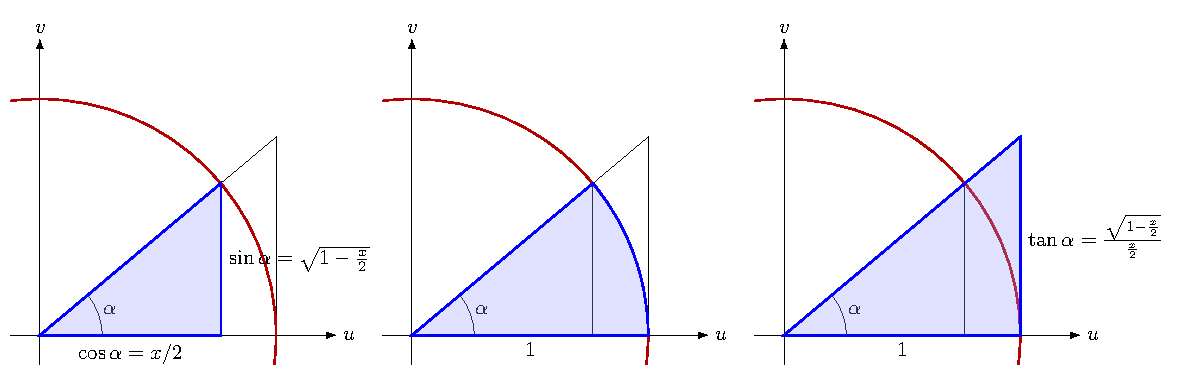
\includegraphics[width=0.8\textwidth]{Ex2unitcircle.pdf}
\end{center}

Per tant, per a $x=2\cos{t}$: 

\[
\int \frac{1}{x^2 \sqrt{4-x^2}}dx = -\frac{1}{4} \tan{t} = -\frac{1}{4}\frac{\sqrt{1-\frac{x}{2}}}{\frac{x}{2}}
\]

%\end{Answer}

\Exercise[title={$\int \frac{dx}{ax^2 + bx + c}$, amb denominador sense arrels reals (arctangent)}]
%\begin{Exercise}[label=Ex6]
  \vspace{5mm}
  $\int \frac{3}{x^2+2x+4} dx$
  

%\end{Exercise}

\Answer

%\begin{Answer}[ref=Ex6]

    En no haver zeros reals del polinoni del denominador ens cal usar l'estratègia de completar quadrats. Aquesta tècnica ens permet acostar l'expressió de la integral a la que tindria una primitiva arctangent.
    En general,
    \[
      ax^2+bx+c=a\left(x^2+\frac{b}{a}x+\frac{c}{a}\right)=a\left((x+r)^2+s^2\right)
    \]
    on es pot veure fàcilment que $r=\frac{b}{2a}$ i $s=\sqrt{\frac{c}{a}-\frac{b^2}{4a^2}}$.En aquest cas, $r=1$ i $s=\sqrt{3}$. Per tant:

    \[
      \int \frac{3}{x^2+2x+4} dx=3\int \frac{1}{(x+1)^2+(\sqrt{3})^2} dx\stackrel{(*)}{=} \frac{1}{\sqrt{3}}\arctan{\frac{x+1}{\sqrt{3}}}+C
    \]
    \begin{description}
      \item[$(*)$] Immediata, ja que $\int \frac{dx}{s^2+x^2}=\frac{1}{s}\arctan{\frac{x+r}{s}}+C$:
    \end{description}

\blacksquare



\Exercise[title={$\int \sin^m x \cos^n x dx$ amb \(m , n \in Z^+\) i $m$ o $n$ senar}]

%\begin{Exercise}[label=Ex3]

$\int \sin^5{x}dx$ 

%\end{Exercise}

\Answer
%  \begin{Answer}[ref=Ex3]

  Usarem que $\sin^2{x}+\cos^2{x}=1$ i l'expressió quedarà:

  \[
    I=\int \sin^5{x}dx = \int \left(1-\cos^2{x}\right)^2\sin{x}dx
  \]

  Veiem que, d'aquesta manera, ens queda una expressió que barreja sinus i cosinus, i sabem que un és la derivada de l'altre. Per tant, una bona substició és $t=\cos{x}; \; dt=-\sin{x}dx$
  \[
    I=\int \sin^5{x}dx = - \int \left(1-t^2\right)^2dt=-\frac{t^5}{5}+2 \frac{t^3}{3}-t+C= -\frac{\cos^5{x}}{5}+2 \frac{\cos^3{x}}{3}-\cos{x}+C
  \]


%\end{Answer}

\Exercise[title={$\int \sin^m x \cos^n x dx$ amb \(m , n \in Z^+\) i $m,n$ parells}]

%\begin{Exercise}[label=Ex4]

Avalúa la integral $\int{ \frac{1}{\sqrt{1-x^2}}dx}$

%\end{Exercise}

\Answer 
%\begin{Answer}[ref=Ex4]

    Considerem el canvi de variable
    \[x=\sin{u}; \; dx=\cos{u} du\].
    Per tant:
  \[
  I=\int \frac{1}{\sqrt{1-x^2}} dx = \int \frac{1}{\sqrt{1-\sin^2{u}}} \cos{u} du = \int \frac{1}{\sqrt{\cos^2{u}}} \cos{u}   du = \int du = u + C
  \]
  si desfem la substitució:
  \[
  I= \arcsin{x} + C
  \]

%\end{Answer}

\Exercise[title={Racional trigonomètrica $\int R(sin x, cos x) dx$}]

%\begin{Exercise}[label=Ex5]

Avalúa la integral $I = \int \frac{2}{1+3\cos{x}} dx$

(Pista: si $t = \tan{\theta/2}$, per raons trigonomètriques obtenim:

\begin{eqnarray*} \sin{\theta}&=&\frac{2t}{1+t^2}\\ \cos{\theta}&=&\frac{1-t^2}{1+t^2}\\ \tan{\theta}&=&\frac{2t}{1-t^2} \end{eqnarray*})





%\end{Exercise}

\Answer
%  \begin{Answer}[ref=Ex5]

    En els casos en que tenim \( I = \int \frac{1}{a+b\cos{x}} dx\) o bé \( I = \int \frac{1}{a+b\sin{x}} dx\) és pràctic usar la substitució \(t = \tan{x/2}\). Aleshores tenim:

    $$ dt=\frac{1}{2} \sec^2{\frac{x}{2}} dx = \frac{1}{2} \left( 1+\tan^2{\frac{x}{2}} \right) dx = \frac{1+t^2}{2} dx     $$

    i, per tant, \(dx=\frac{2}{1+t^2} dt\)

    \begin{eqnarray*}
    I &=& \int \frac{2}{1+3\cos{x}} dx = \int \frac{2}{(1+3\frac{1-t^2}{1+t^2})} \frac{2}{(1+t^2)} dt \\
    &=& 4 \int \frac{1}{1+t^2+3-3t^2}  dt =  4 \int \frac{1}{4-2t^2}  dt = \int \frac{1}{1-\left(\frac{t}{\sqrt{2}}\right)^2} dt
    \end{eqnarray*}

    i ara fem la substitució \(u=\frac{t}{\sqrt{2}}\) i \( du = \frac{dt}{\sqrt{2}}\)

    \begin{eqnarray*}
    I &=&  \int \frac{1}{1-\left(\frac{t}{\sqrt{2}}\right)^2} dt = \frac{1}{\sqrt{2}}  \int \frac{1}{1-u^2} du = \frac{1}{\sqrt{2}} \text{arctanh} \, {u} + C \\
    &=& \frac{1}{\sqrt{2}} \text{arctanh} {\frac{t}{\sqrt{2}}} + C =  \frac{1}{\sqrt{2}} \text{arctanh}  {\frac{\tan{x/2}}{\sqrt{2}}} + C
    \end{eqnarray*}

%\end{Answer}

\Exercise[title={$\int \sin^m x \cos^n x dx$ amb \(m , n \in Z^+\) i $m,n$ parells}]

%\begin{Exercise}[label=Ex6]

$\int \cos^4{x}dx$ (pista: per a funcions sinusoidals d'exponent parell, usa les expressions $\sin^2{x}=\frac{1}{2}(1-\cos{2x})$ o bé $\cos^2{x}=\frac{1}{2}(1+\cos{2x})$ per reduir l'exponent.)


%\end{Exercise}

\Answer

%\begin{Answer}[ref=Ex6]

    Usant
    \[
    \cos^4{x} =\left(\cos^2{x}\right)^2
              =\left(\frac{1}{2}(1+\cos{2x})\right)^2
              =\frac{1}{4}\left(1+\cos^2{2x}+2\cos{2x}\right)
    \]
    Altre cop:
    \[
    \cos^2{2x} = \frac{1}{2}(1+\cos{4x})
    \]
    Per tant:
    \begin{eqnarray*}
      I&=&\int \cos^4{x}dx \\
      &=& \frac{1}{4} \int \left(1+\frac{1}{2}(1+\cos{4x})+2\cos{2x}\right) dx\\
      &=& \frac{1}{4} \int \left(\frac{3}{2}+\frac{1}{2}\cos{4x}+2\cos{2x}\right) dx\\
      &=& \frac{1}{4} \left(\frac{3}{2}x +\frac{1}{8}\sin{4x}+\sin{2x}\right)+C
    \end{eqnarray*}

%\end{Answer}


\subsection{Integral definida}



\Exercise[title={Integral delimitada entre funcions}]

%\begin{Exercise}[label=Ex7]
\Question
Sigui $S$ la regió delimitada  per les corbes $f_1(x)=x^2$, $f_2(x)=x$. Calculeu $\int \int_S (x+1)y dxdy$

%\end{Exercise}

\Answer

%  \begin{Answer}[ref=Ex7]

Comencem per dibuixar les dues funcions.

    \begin{center}
      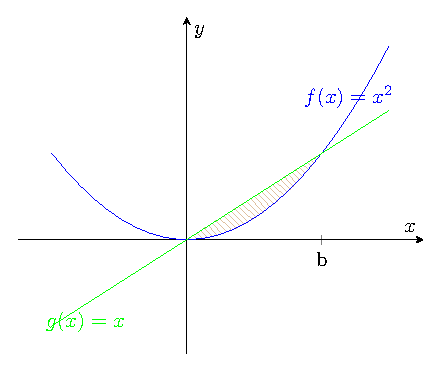
\includegraphics[width=0.5\textwidth]{areax2x.pdf}
    \end{center}

Es tallen en els punts $(0,0)$ i $(1,1)$, ja que
\[
  x^2=x \Rightarrow x^2-x=0 \Rightarrow x(x-1)=0
\]

La integració haurà de tenir en compte que la variable $x$ depèn de la $y$ i viceversa, per trobar el volum de l'objecte de la figura:

\begin{center}
  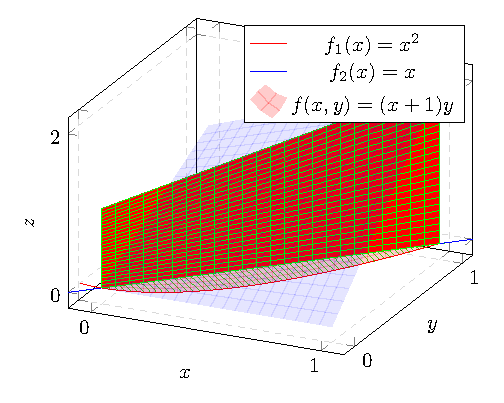
\includegraphics[width=0.5\textwidth]{volum3Dxx2xmes1y.pdf}
\end{center}

Per tant, una manera de solucionar el problema és:
\begin{eqnarray*}
V=\int \int_S (x+1)y dx dy &=& \int_{x=0}^{x=1} \left[ \int_{y=x^2}^{y=x} (x+1)y dy \right]dx \\
&=& \int_{x=0}^{x=1} \left[ \frac{(x+1)y^2}{2} \right]_{x^2}^{x} dx \\
&=& \frac{1}{2}\int_{x=0}^{x=1} \left[ (x+1)x^2 - (x+1)x^4 \right] dx\\
&=& \frac{1}{2}\int_{x=0}^{x=1} \left[ -x^5-x^4+x^3+x^2  \right] dx\\
&=& \frac{1}{2} \left[ -\frac{x^6}{6}-\frac{x^5}{5}+\frac{x^4}{4}+\frac{x^3}{3}\right]_{x=0}^{x=1}\\
&=& \frac{1}{2}\left[ \left(-\frac{1}{6}-\frac{1}{5}+\frac{1}{4}+\frac{1}{3}\right)-\left(0\right)\right]=\frac{13}{120}
\end{eqnarray*}


%\end{Answer}

\Exercise[title={Integral delimitada entre funcions}]

%\begin{Exercise}[label=Ex7]

Sigui $R$ la regió delimitada  per les corbes $f(x)=x^2+2x-3$, $g(x)=3x+3$. 
\begin{itemize}
  
  \item Representeu gràficament la regió $R$.
  \item Determineu l'àrea $A(R)$ de la regió $R$.
  \item Calculeu $\int \int_R x dxdy$ .
\end{itemize}


%\end{Exercise}

\Answer

%  \begin{Answer}[ref=Ex7]
\begin{itemize}
  \item 
Comencem per dibuixar les dues funcions.

    \begin{center}
      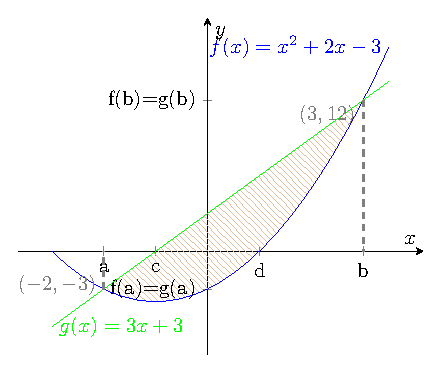
\includegraphics[width=0.5\textwidth]{areax2plus2xminus33xplus3.pdf}
    \end{center}

A partir de solucionar 
\[
  x^2+2x-3=3x+3
\]
trobem que es tallen en els punts $(-2,-3)$ i $(3,12)$.

\item Per trobar l'àrea podem pensar en dividir el càlcul en tres parts, 
si ens fan dubtar els signes de les funcions:

\[
  A(R)=\int_a^c [f(x)-g(x)] dx +  \int_c^d [g(x)+f(x)] dx + \int_d^b [g(x)-f(x)] dx
\]

o bé, més pràctic, podem sumar un valor superior a 4 a les dues funcions per tal que ens quedin les dues damunt de l'eix de les abscisses.\footnote{Només cal trobar el mínim de la funció parabòlica que es dona quan $f'(x)=2x+2=0$, que passa a $x=-1$, on $f(x)=-4$.}
Per tant, l'àrea serà igual a
\[
  A(R) = \int_a^b [(g(x)+4)-(f(x)+4)] dx = \int_a^b [g(x)-f(x)] dx 
  \] 
  \[
    A(R) = \int_{-2}^{3} [(3x+3)-(x^2+2x-3)] dx =  \int_{-2}^{3} [-x^2+x+6] dx = \left[-\frac{x^3}{3}+\frac{x^2}{2}+6x\right]_{-2}^3= \frac{125}{6}
    \] 
  
\item Com que ens donen dues funcions de la variable $x$, el més pràctic és integrar primer respecte $y$ i despreś respecte $x$:

\begin{eqnarray*}
V=\int \int_R x dx dy &=& \int \int_R x dy dx\\
&=& \int_{x=-2}^{x=3} \left[ \int_{x^2+2x-3}^{3x+3} x dy \right]dx  \\
&=& \int_{x=-2}^{x=3} x [(3x+3)-(x^2+2x-3)] dx \\
&=& \left[-\frac{x^4}{4}+\frac{x^3}{3}+3x^2\right]_{-2}^3\\
&=& \left(-\frac{3^4}{4}+\frac{3^3}{3}+3^3\right)-\left(-\frac{(-2)^4}{4}+\frac{(-2)^3}{3}+3 (-2)^2\right)
=\frac{125}{12}
\end{eqnarray*}
\end{itemize}


%\end{Answer}


\subsection{Integració de moltes variables}

\Exercise[title={Volum esfera}]
%\begin{Exercise}[label=Ex7]

  Calcula el volum d'una esfera de radi $a$ usant una integral triple.

%\end{Exercise}

\Answer

El volum de l'esfera ve donat per l'expressió:

\[
  V=\int\int\int_{\Omega} dV 
\]



Si explorem el problema usant coordenades cartesianes, l'element de volum és $\dif V= \dif x \dif y \dif z$ i els límits d'integració quedarien com:

\[
  V=\int_{-a}^a  \int_{-\sqrt{a^2-x^2}}^{\sqrt{a^2-x^2}} \int_{-\sqrt{a^2-x^2-y^2}}^{\sqrt{a^2-x^2-y^2}} \dif z \dif y \dif x 
\]

Alternativament, podem observar que la simetria de l'objecte ens permet usar coordenades esfèriques:

\begin{center}
  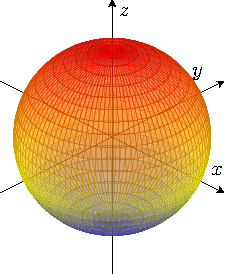
\includegraphics[width=0.3\linewidth]{sphere.pdf}
  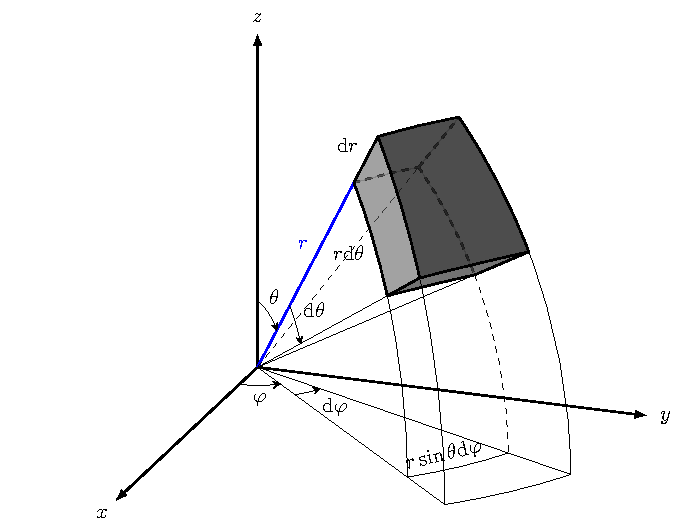
\includegraphics[width=0.6\linewidth]{CoordinatesSpherical.pdf}
\end{center}

Ara l'element de volum vindrà donat per $\dif V = r^2 \sin{\theta} \dif r \dif \theta \dif \varphi$ i els límits d'integració canviaran de forma molt favorable, ja que:

\[
\begin{cases}
  -a \leq x \leq a\\
  -\sqrt{a^2-x^2} \leq y \leq \sqrt{a^2-x^2} \\
  0 \leq z \leq a^2-x^2 - y^2\\
\end{cases}  
\Rightarrow
\begin{cases}
  0 \leq \theta \leq \pi\\
  0 \leq r \leq a \\
  0 \leq \varphi \leq 2\pi\\
\end{cases}  
\]

Així:

\begin{eqnarray*}
  V&=&\int_{0}^{2\pi}  \int_{0}^{\pi} \int_0^{a} r^2 \sin{\theta} \dif r \dif \theta \dif \varphi = \int_{0}^{2\pi} \dif \varphi  \int_{0}^{\pi} \sin{\theta} \dif \theta \int_0^{a} r^2  \dif r   \\
  &=& [\varphi]_0^{2\pi} \left[-\cos{\theta}\right]_0^{\pi} \left[\frac{r^3}{3}\right]_0^a =\boxed{\frac{4}{3}\pi a^3}
\end{eqnarray*}

%\end{Answer}

\Exercise[title={Volum paraboloide}]
%\begin{Exercise}[label=Ex7]

  Calcula el volum delimitat pel paraboloide $z=x^2+y^2$. i el pla $z=1$.

%\end{Exercise}

\Answer

Dibuixem primer el gràfic:

\begin{center}
  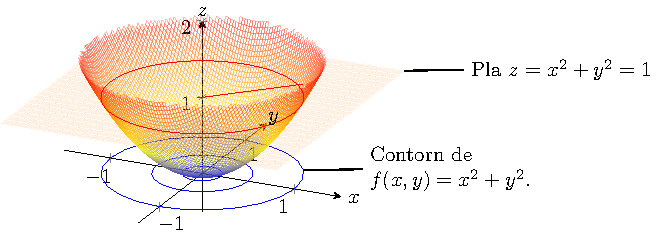
\includegraphics[width=0.9\linewidth]{paraboloid.pdf}
\end{center}

El volum del paraboloide vindria donat per l'expressió:

\[
  V=\int\int\int_{\Omega} dV 
\]

Si explorem el problema usant coordenades cartesianes, l'element de volum és $\dif V= \dif x \dif y \dif z$ i els límits d'integració quedarien com:

\[
  V=\int_{-1}^1  \int_{-\sqrt{1-x^2}}^{\sqrt{1-x^2}} \int_0^{x^2+y^2} \dif z \dif y \dif x 
\]

Podem intentar fer aquesta integral, però clarament el fet que apareguin arrels en els límits d'integració no facilita gens la feina (tot i que la integral no és pas molt complicada). Pots solucionar-la amb \texttt{Matlab} usant aquest breu codi:
\begin{lstlisting}[language=Matlab]
 syms x y z
 intZ = int(1,z,0,x^2+y^2)
 intY = int(intZ,y,-sqrt(1-x^2),sqrt(1-x^2))
 intX=int(intY)
 volum = int(intY,x,-1,1)
\end{lstlisting}

Alternativament, podem observar que la simetria de l'objecte ens permet usar coordenades cilíndriques, molt més pràctiques:

\begin{center}
  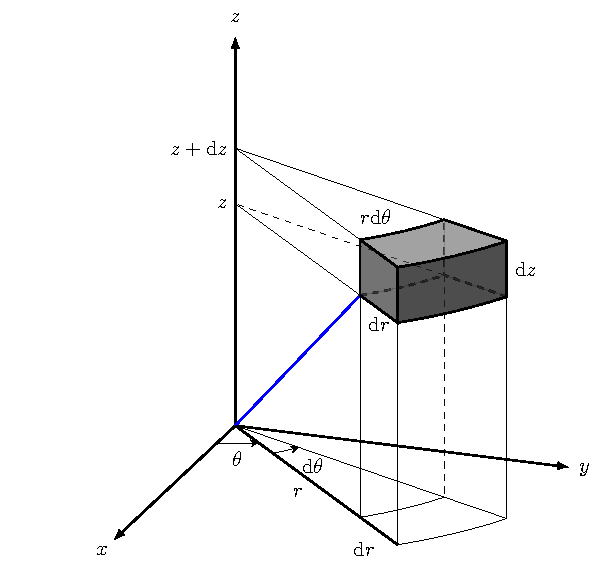
\includegraphics[width=0.5\linewidth]{CoordinatesCylindrical.pdf}
\end{center}

Ara l'element de volum vindrà donat per $\dif V = r \dif z \dif r \dif \theta$ i els límits d'integració canviaran de forma molt favorable, ja que:

\[
\begin{cases}
  -1 \leq x \leq 1\\
  -\sqrt{1-x^2} \leq y \leq \sqrt{1-x^2} \\
  0 \leq z \leq x^2 + y^2\\
\end{cases}  
\Rightarrow
\begin{cases}
  0 \leq \theta \leq 2 \pi\\
  0 \leq r \leq 1 \\
  0 \leq z \leq x^2 + y^2 = r^2\\
\end{cases}  
\]

Així:

\begin{eqnarray*}
  V&=&\int_{0}^{2\pi}  \int_{0}^{1} \int_0^{r^2} r \dif z \dif r \dif \theta = \int_{0}^{2\pi} \dif \theta  \int_{0}^{1} r \left[\int_0^{r^2} \dif z\right] \dif r \\
  &=& \theta]_{0}^{2\pi} \int_{0}^{1} r z]_0^{r^2} \dif r = 2\pi \left[\frac{r^4}{4}\right]_0^1=\boxed{\frac{\pi}{2}}
\end{eqnarray*}

%\end{Answer}


\end{ExerciseList}

\section{Material pràctic}

\begin{itemize}
    \item La Figura \ref{Fig:unitcircle} conté informació sobre els sinus i cosinus d'alguns dels valors d'angles més comuns en els exercicis de l'assignatura.
\end{itemize}

\begin{figure}
    \begin{minipage}[r]{0.7\textwidth}
      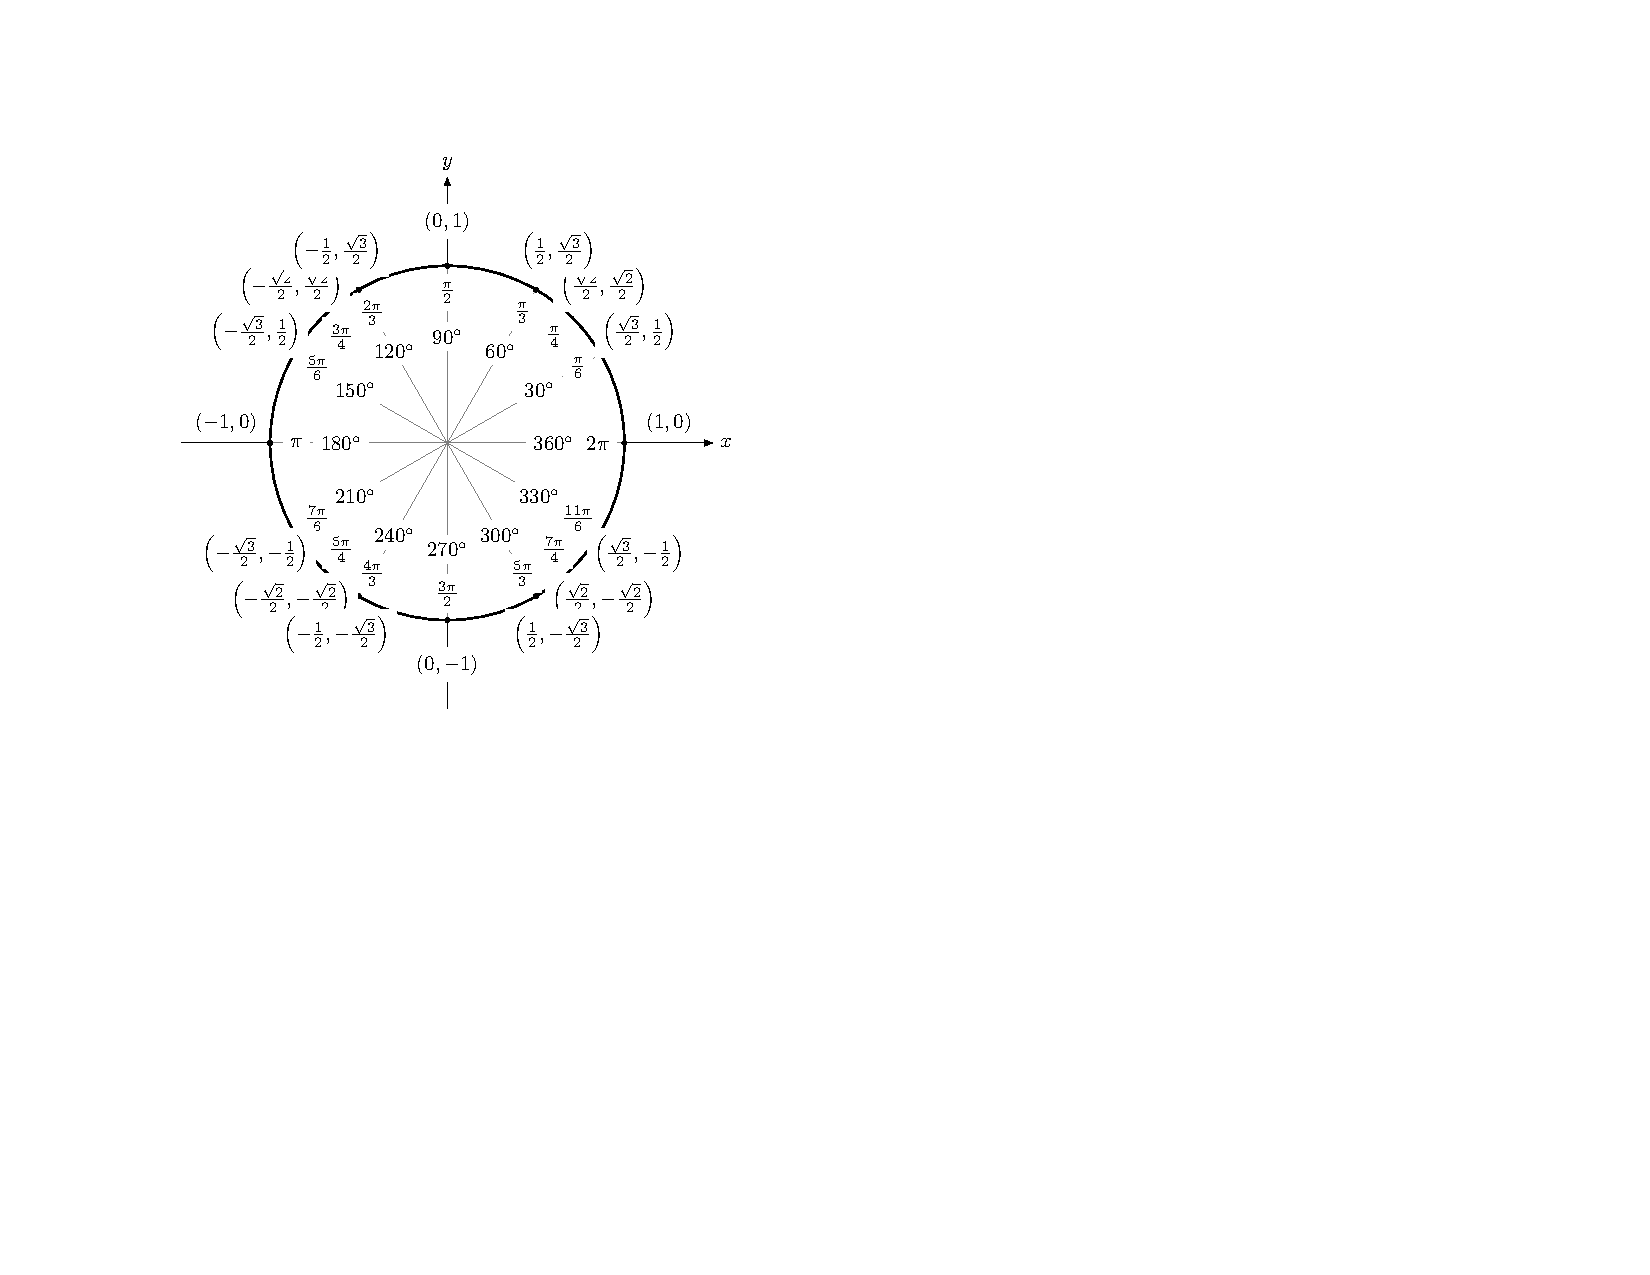
\includegraphics[width=\textwidth]{unitcircletikz}
    \end{minipage}\hfill
    \begin{minipage}[l]{0.3\textwidth}
      \caption{
        Esquema dels valors de $\sin x$ i $\cos x$ per a alguns valors d'angles.
      } \label{Fig:unitcircle}
    \end{minipage}
  \end{figure}
  
\end{document}
